%=====================================================================
% Arquivo: main.tex
% Autor  : Macilon Araújo Costa Neto
% Data   : 02/07/2012
%=====================================================================
\documentclass[header=ruled]{abnt}
%=====================================================================
% Utilização de pacotes.
%=====================================================================
\usepackage[T1]{fontenc}		% fontes PS com acentos
\usepackage[english,brazil]{babel}	% idiomas permitidos
\usepackage[utf8]{inputenc}	% edição direta com acentos
%\usepackage{latexsym}		% símbolos extras do LaTeX
\usepackage{amssymb}			% símbolos AMS do LaTeX
\usepackage{pifont}			% símbolos checkmarks
\usepackage{epsfig}			% tratamento de figuras EPS
%\usepackage{multicol}		% tratamento de vários colunas
\usepackage{fancyvrb}		% códigos Verbatim
\usepackage{array}			% ambiente tabular avançado
%\usepackage{singlespace}	% espaçamento simples
\usepackage{fancyhdr}		% tratamento de cabeçalho
\usepackage{subfigure}		% tratamento de subfiguras
\usepackage{multirow}		% tratamento de várias linhas
\usepackage{enumitem}		% tratamento dos enumeradores
%\usepackage{rotating}		% rotacionar figuras/tabelas/etc
\usepackage{listings}		% para inserir código no texto latex


\usepackage{color}
\definecolor{dkgreen}{rgb}{0,0.6,0}
\definecolor{gray}{rgb}{0.5,0.5,0.5}
\definecolor{mauve}{rgb}{0.58,0,0.82}

\lstset{ %
  language=XML,% the language of the code
  basicstyle=\footnotesize,% the size of the fonts that are used for the code
  numbers=left,% where to put the line-numbers
  numberstyle=\tiny\color{gray},% the style that is used for the line-numbers
  stepnumber=1,% the step between two line-numbers. If it's 1, each line 
                                  % will be numbered
  numbersep=5pt,% how far the line-numbers are from the code
  backgroundcolor=\color{white},      % choose the background color. You must add \usepackage{color}
  showspaces=false,               % show spaces adding particular underscores
  showstringspaces=false,         % underline spaces within strings
  showtabs=false,                 % show tabs within strings adding particular underscores
  frame=single,                   % adds a frame around the code
  rulecolor=\color{black},        % if not set, the frame-color may be changed on line-breaks within not-black text (e.g. comments (green here))
  tabsize=1,                      % sets default tabsize to 2 spaces
  captionpos=b,                   % sets the caption-position to bottom
  breaklines=true,                % sets automatic line breaking
  breakatwhitespace=false,        % sets if automatic breaks should only happen at whitespace
  title=\lstname,                   % show the filename of files included with \lstinputlisting;
                                  % also try caption instead of title
  keywordstyle=\color{blue},% keyword style
  commentstyle=\color{dkgreen},% comment style
  stringstyle=\color{mauve},% string literal style
  escapeinside={\%*}{*)},% if you want to add LaTeX within your code
  morekeywords={*,...},% if you want to add more keywords to the set
  deletekeywords={...}% if you want to delete keywords from the given language
}



%=====================================================================
% Dados gerais sobre o documento da tese
%---------------------------------------------------------------------
%=====================================================================
% Dados sobre o Programa de Pós-Graduação
%=====================================================================

% Nome da Instutuição
\newcommand{\instituicaoA}
           {Universidade Federal do Rio Grande do Norte}

% Nome do Centro
\newcommand{\centro}
           {Centro de Ciências Exatas e da Terra}

% Nome do Departamento
\newcommand{\departamento}
           {Departamento de Informática e Matemática Aplicada}

% Nome do Programa
\newcommand{\programa}
           {Programa de Pós-graduação em Sistemas e Computação}

% Nome do Coordenador do Programa
\newcommand{\coordenador}
           {Prof. David Boris Paul Déharbe}

% Grau obtido pelo programa
\newcommand{\grau}
           {Mestre em Ciência da Computação} %~(Mr.)}

% Grau (em inglês) obtido pelo programa
\newcommand{\grauEMingles}
           {Philosophy Doctor in Computer Science} %~(Ph.D)}

%=====================================================================
% Dados sobre a Banca Examinadora (não incluir orientador)
%=====================================================================

% Nome do Presidente
\newcommand{\presidente}
           {\orientadorA\ -- UFRN}

% Nome do 2º Membro
\newcommand{\membroDOIS}
           {Prof. Martin Alejandro Musicante -- UFRN}

% Nome do 3º Membro
\newcommand{\membroTRES}
           {Prof. Placido Neto -- IFRN}

% Nome do 4º Membro
\newcommand{\membroQUATRO}
           {Profª. A definir}

% Nome do 5º Membro
%\newcommand{\membroCINCO}
%           {Profª. Milene Selbach Silveira -- PUCRS}

%=====================================================================
% Dados sobre a Dissertação
%=====================================================================

% Nome do Autor da Dissertação
\newcommand{\autorA}
           {Rodrigo Farias Herculano Mendes}

% Nome do Autor (para Ficha Catolográfica) da Dissertação
\newcommand{\autorFicha}
           {HERCULANO MENDES, Rodrigo Farias}

% Título da Dissertação 
\newcommand{\tituloA}
           {Uma abordagem orientada a modelos para a geração automática de composições de serviços em WS-BPEL}

% Título (em inglês) da Dissertação
\newcommand{\tituloEMingles}
           {A model-driven approach for the automatic generation of service compositions in WS-BPEL}

% Título da Dissertação para Ficha Catalográfica (apenas primeria letra maiúscula)
\newcommand{\tituloFicha}
           {Uma abordagem orientada a modelos para a geração automática de composições de serviços em WS-BPEL}

% Área da Dissertação
\newcommand{\area}
           {Engenharia de Software}

% Área (em inglês) da Dissertação
\newcommand{\areaEMingles}
           {Software Engineering}

% Palavras Chaves da Dissertação
\newcommand{\palavras}
           {Orientação a serviços, desenvolvimento dirigido a modelos, metodologia, SOD-M, WS-BPEL.}

% Palavras Chaves para ficha catalográfica
\newcommand{\palavrasFicha}    
           {2.  Orientação a serviços.   3. desenvolvimento dirigido a modelos.  4.
             Desenvolvimento  baseado  em  modelos. 5.   Avaliação  de
             usabilidade.}

% Palavras Chaves (em inglês) da Dissertação
\newcommand{\palavrasEMingles} 
           {Service orientation, driven development models, methodology, SOD-M, WS-BPEL.}

% Nome do Orientador
\newcommand{\orientadorA}
           {Prof. Umberto Souza da Costa}

% Nome do Orientador para Ficha Catalográfica
\newcommand{\orientadorFicha}
           {Costa, Umberto Souza}

% Local
\newcommand{\localA}
           {Natal}

% Data
\newcommand{\dataA}
           {Agosto de 2013}

% Data (em inglês)
\newcommand{\dataEMingles}
           {August, 2013}
% Ano para Ficha Catalográfica
\newcommand{\ano}
           {2013}
				% Arquivo com todos os dados
%---------------------------------------------------------------------
\usepackage[pdftitle={\tituloA},
  pdfauthor={\autorA},
  pdfsubject={Tese de Doutorado em Ciência da Computação},
  pdfkeywords={\palavras},
  bookmarks,
  colorlinks,
  breaklinks=true,
  linkcolor=black,
  citecolor=black,
  filecolor=black,
  urlcolor=black]{hyperref}		% usados para geração do PDF
\usepackage[abnt-full-initials=yes,
  abnt-etal-text=emph,
  abnt-etal-list=0,
  abnt-etal-cite=3]{abntcite}		% bibliografia do abntex
%=====================================================================
% Vários comandos utilizados no documento, incluído abreviaturas
%---------------------------------------------------------------------
%=====================================================================
% Macros usadas no documento
%---------------------------------------------------------------------
% Para expressões em inglês:
% \en{hardware}, \en{software}
%---------------------------------------------------------------------
\newcommand{\en}[1]{
  \selectlanguage{english}
  \textit{#1}
  \selectlanguage{brazil}
}
%---------------------------------------------------------------------
% Definindo o comando figura
% 1 - Legenda da figura
% 2 - Rótulo para referência da figura
% 3 - Nome de arquivo que contém a figura
% 4 - Escala da figura
% 5 - Ângulo de rotação da figura
%---------------------------------------------------------------------
\newcommand{\figura}[5]{
  \begin{figure}[!htb]
    \begin{center}
      \includegraphics[scale=#4,angle=#5]{images/#3}
      \caption{#1}
      \label{#2}
    \end{center}
  \end{figure}
}
%---------------------------------------------------------------------
% Versão estendida para expandir em documentos com duas colunas
%---------------------------------------------------------------------
\newcommand{\figuraL}[5]{
  \begin{figure*}[!htb]
    \begin{center}
      \includegraphics[scale=#4,angle=#5]{images/#3}
      \caption{#1}
      \label{#2}
    \end{center}
  \end{figure*}
}
%---------------------------------------------------------------------
% Símbolos para 
%---------------------------------------------------------------------
\newcommand{\X}{~~$\bullet$}
\newcommand{\cf}{\ding{52}}
\newcommand{\vi}{\ding{56}}
\newcommand{\na}{{\bf --}}
%---------------------------------------------------------------------
% Siglas e significados
%---------------------------------------------------------------------
% OMG Stardarts
%---------------------------------------------------------------------
\newcommand{\omg}{OMG}
\newcommand{\Omg}{Object Management Group}
\newcommand{\mda}{MDA}
\newcommand{\Mda}{Model Driven Architecture}
\newcommand{\mof}{MOF}
\newcommand{\Mof}{Meta Object Facility}
\newcommand{\uml}{UML}
\newcommand{\Uml}{Unified Modeling Language}
\newcommand{\ocl}{OCL}
\newcommand{\Ocl}{Object Constraint Language}
\newcommand{\xmi}{XMI}
\newcommand{\Xmi}{\xmi\ Metadata Interchange}
\newcommand{\xml}{XML}
\newcommand{\Xml}{Extensible Markup Language}
\newcommand{\qvt}{QVT}
\newcommand{\Qvt}{Query/View/Transformation}
%---------------------------------------------------------------------
% MDA models
%---------------------------------------------------------------------
\newcommand{\cim}{CIM}
\newcommand{\Cim}{Computation Independent Model}
\newcommand{\pim}{PIM}
\newcommand{\Pim}{Platform Independent Model}
\newcommand{\psm}{PSM}
\newcommand{\Psm}{Platform Specific Model}
%---------------------------------------------------------------------
% Eclipse Modeling
%---------------------------------------------------------------------
\newcommand{\emf}{EMF}
\newcommand{\Emf}{Eclipse Modeling Framework}
\newcommand{\gef}{GEF}
\newcommand{\Gef}{Graphical Editing Framework}
\newcommand{\gmf}{GMF}
\newcommand{\Gmf}{Graphical Modeling Framework}
\newcommand{\pojo}{POJO}
\newcommand{\Pojo}{Plain Old Java Object}
%---------------------------------------------------------------------
% Model-based
%---------------------------------------------------------------------
\newcommand{\diubm}{DIUBM} 
\newcommand{\Diubm}{Desenvolvimento de Interface de Usuário Baseado em
  Modelos}
\newcommand{\mbuid}{MBUID}
\newcommand{\Mbuid}{Model-Based User Interface Development}
\newcommand{\mdd}{MDD}
\newcommand{\Mdd}{Model Driven Development}
%---------------------------------------------------------------------
% Gerais de IHC
%---------------------------------------------------------------------
\newcommand{\aladim}{ALaDIM}
\newcommand{\Aladim}{Abstract Language  for Description of Interactive
  Message}
\newcommand{\molic}{MoLIC}
\newcommand{\Molic}{Modeling Language for Interaction as Conversation}
\newcommand{\imml}{IMML}
\newcommand{\Imml}{Interactive Message Modeling Language}
\newcommand{\ihc}{IHC}
\newcommand{\Ihc}{Interação Humano-Computador}
\newcommand{\chimy}{CHI}
\newcommand{\Chimy}{Computer-Human Interaction}
\newcommand{\ec}{Engenharia Cognitiva}
\newcommand{\ta}{Teoria da Ação}
%---------------------------------------------------------------------
% Software Engineering
%---------------------------------------------------------------------
\newcommand{\rup}{RUP}
\newcommand{\Rup}{Rational Unified Process}
\newcommand{\es}{ES}
\newcommand{\Es}{Engenharia de Software}
\newcommand{\ese}{ESE}
\newcommand{\Ese}{Engenharia de Software Experimental}
\newcommand{\gui}{GUI}
\newcommand{\Gui}{Graphical User Interface}
%---------------------------------------------------------------------
% Semiotic Engineering
%---------------------------------------------------------------------
\newcommand{\se}{Engenharia Semiótica}
\newcommand{\mac}{MAC}
\newcommand{\Mac}{Método de Avaliação da Comunicabilidade}
\newcommand{\mis}{MIS}
\newcommand{\Mis}{Método de Inspeção Semiótica}
%---------------------------------------------------------------------
% Gerais
%---------------------------------------------------------------------
\newcommand{\cdn}{CDN}
\newcommand{\Cdn}{Cognitive Dimensions of Notations}
\newcommand{\gqm}{GQM}
\newcommand{\Gqm}{Goal/Question/Metric}


\newcommand{\linkert}{\\(~~) Pouquíssimo (~~) Pouco (~~) Neutro (~~) Muito
  (~~) Demasiado}
%=====================================================================

%=====================================================================
% Início do documento
%---------------------------------------------------------------------
\begin{document}        
%\doublespacing			% Para atender a solicitação do Jair
%=====================================================================
% Definições para as páginas para o pré-textual do trabalho
%---------------------------------------------------------------------
\pagestyle{empty}
\pagenumbering{roman}
%=====================================================================
% Conteúdo pré-textual
%---------------------------------------------------------------------
%=====================================================================
% Capa
%=====================================================================

\begin{titlepage}
  \begin{center}
  {
    \fontsize{16}{18}
    \selectfont 
    \bfseries

    \autorA

  }

  \vfill

  \begin{espacosimples}
    {
      \fontsize{18}{22}
      \selectfont
      \bfseries

      \tituloA

    }
  \end{espacosimples}

  \vfill

  {
    \fontsize{14}{16}
    \selectfont
    \bfseries 
    
    \localA \\ \dataA
    
  }

\end{center}

\end{titlepage}

\setcounter{page}{1}
%=====================================================================
% Folha de Rosto
%=====================================================================

\begin{titlepage}
\begin{center}
  \begin{espacosimples}

    {
      \fontsize{14}{16}
      \selectfont 
      \bfseries
     
      \instituicaoformat

      \instituicaoA\\
      \centro\\
      \departamento\\
      \programa
      
    }
    
    \vfill

    {
      \fontsize{18}{22}
      \selectfont
      \bfseries
      
      \tituloA
      
    }
    
    \vfill

    {
      \fontsize{14}{16}
      \selectfont
      \bfseries 
      
      \autorA
      
    }

    \vfill

    \begin{flushright}

      \parbox{8cm}{

	{
	  \fontsize{10}{12}
	  \selectfont
   
	  Dissertação   submetida   ao   \programa\  do   \departamento\   do
          \centro\ da \instituicaoA\ como  parte dos requisitos para a
          obtenção do título de \grau.

	}
      }
    \end{flushright}

    \vfill

    {
      \fontsize{14}{16}
      \selectfont
%      \bfseries 
      
      \orientadorA\\Orientador
      
    }

    \vfill

    {
      \fontsize{12}{14}
      \selectfont
      
      \localA, \dataA

    }

  \end{espacosimples}

\end{center}

\end{titlepage}

%=====================================================================
% Ficha Catalográfica
%=====================================================================

\vspace*{\fill}


\begin{center}
  \begin{singlespace}  
  
    Catalogação  da Publicação na  Fonte.  UFRN  / SISBI  / Biblioteca
    Setorial\\Especializada do Centro de Ciências Exatas e da Terra --
    CCET.

  \end{singlespace}
\end{center}                 

\framebox[1.1\width]{
        
\begin{minipage}{380pt}

  \begin{singlespace}

    \vspace{10pt}

    \autorFicha. \\
    \tituloFicha. 
    -- \localA, RN, \ano. \\

    120 f. : il. \\

    Orientador: \orientadorA \\

    Dissertação~(Mestre) -- 
    \instituicaoA. 
    \centro. 
    \departamento. 
    \programa.\\

    1. \area\ -- Dissertação. 
    \palavrasFicha\ 
    I.~\orientadorFicha. 
    II.~Título. \\

  \end{singlespace}

  RN/UF/BSE-CCET \hspace{79mm} CDU 004.4 \\

\end{minipage}
}
 %% Ficha Catalográfica
%=====================================================================
% Folha de Aprovação
%=====================================================================

\begin{center}

  \begin{singlespace}
  {
    \fontsize{14}{16}
    \selectfont
    
    {\bf \autorA}
    \\~\\
  }

  \vfill  

  {
    \fontsize{16}{18}
    \selectfont

    {\bf \tituloA}

  }

  \end{singlespace}

\end{center}

\vfill

{
  \fontsize{12}{14}
  \selectfont
  
  \noindent Esta Dissertação foi defendida e julgada adequada para a obtenção
  do título de \grau\ e aprovada em sua forma final pelo \programa\ do
  \departamento\ do \centro\ da \instituicaoA, em 26 de agosto de 2013.
  
}

\vfill

\begin{center}  
  
  {
    \fontsize{11}{13}
    \selectfont
    
    \begin{singlespace}

      ~\\
      \rule{100mm}{0.2mm}\\
      \orientadorA\\
      Orientador\\
      [1.0cm]

      \rule{100mm}{0.2mm}\\
      \coordenador\\
      Coordenador do Programa

    \end{singlespace}
    
  }
  
\end{center}

{
  \fontsize{12}{14}
  \selectfont
  
  \noindent {\bf Banca Examinadora}:
  
  \vfill
  
  \begin{center}
    
    {
      \fontsize{11}{13}
      \selectfont
      
      \begin{singlespace}

	\rule{100mm}{0.2mm}\\
	\presidente\\
	Presidente\\
	[1.0cm]

	\rule{100mm}{0.2mm}\\
	\membroDOIS\\
	[1.0cm]
	
	\rule{100mm}{0.2mm}\\
	\membroTRES\\
	[1.0cm]

	\rule{100mm}{0.2mm}\\
	\membroQUATRO\\
	[1.0cm]

%	\rule{100mm}{0.2mm}\\
%	\membroCINCO\\
      \end{singlespace}

    }
  \end{center}

}

%=====================================================================
% Dedicatória
%=====================================================================

\vspace*{\fill}

{
  \raggedleft

  \begin{singlespace}

%    Este trabalho é dedicado à\\
%    {\em Eliana}, minha amada esposa e ao\\
%    {\em Henrique}, meu abençoado filho.

  \end{singlespace}        

}


\pagestyle{plain}
%%=====================================================================
% Folha de Agradecimentos
%=====================================================================

\chapter*{Agradecimentos}

\noindent A Huguinho, Zezinho e Luisinho, os sobrinhos do Pato Donald.

\noindent  Aos  bravos  gauleses,  Asterix,  Obelix, e  a  seu  chefe,
Abracurcix, pilares da resistência contra as legiões de Júlio César.

\noindent  A Stan, Kyle,  Cartman e  Kenny (Oh,  my God!   They killed
Kenny! {\em You bastards!}).


%=====================================================================
% Resumo
%=====================================================================
%% O  resumo deve  ter frases  indicando:  o contexto;  o problema  ou
%% questão  de pesquisa;  a  justificativa para  a  sua relevância;  a
%% solução que vai ser dada; quais as contribuições e como ela vai ser
%% verificada e validada (revisão do Jair).
%---------------------------------------------------------------------
\begin{resumo}

\vfill

{
  \fontsize{12}{14}
  \selectfont

%  \noindent A teoria da Engenharia Semiótica, considera que o designer
%  comunica ao  usuário, por  meio da interface,  {\em o que}  ele pode
%  fazer e  {\em como} deve  agir para usufruir das  funcionalidades do
%  sistema.  Dessa  forma, a  interface é vista  com uma  {\em mensagem
%    interativa} porque,  além de comunicar estes  aspectos ao usuário,
%  também possibilita  a comunicação entre  o usuário e o  sistema.  No
%  desenvolvimento de um  sistema interativo, estão envolvidos diversos
%  profissionais  e a  comunicação  entre eles  se dá,  principalmente,
%  através do  compartilhamento de artefatos comuns,  como modelos, por
%  exemplo.    O  uso   de   modelos  possibilita   uma  abordagem   de
%  desenvolvimento  na  qual os  modelos  são  usados  por designers  e
%  desenvolvedores.   Na  abordagem baseada  em  modelos,  o modelo  de
%  interação  é   um  artefato  que   cobre  a  maioria   dos  aspectos
%  relacionados  ao  ``o que''  e  ``como''  o  usuário pode  fazer  ao
%  interagir com  a aplicação.  Além disso,  ele pode ser  usado para a
%  identificação  de problemas de  usabilidade durante  o design  e não
%  apenas durante  os testes  de interface e  aceitação, o que  reduz o
%  impacto  nos  custos  de  processo.  Nesse  sentido,  este  trabalho
%  endereça duas questões.  A primeira  é a modelagem da interação, sob
%  uma perspectiva comunicativa, na qual o designer terá que contar com
%  o  desenvolvedor que  irá atuar  como  um tradutor  ao codificar  na
%  interface  sua  mensagem  interativa.   A  segunda  é  identificação
%  antecipada  de  problemas   de  usabilidade,  que  visa  contribuir,
%  principalmente, com  a redução dos custos  de desenvolvimento.  Para
%  isso,  este  trabalho  apresenta  (i)  a linguagem  \aladim,  que  é
%  fundamentada  na \se\  e  busca auxiliar  o  designer na  concepção,
%  representação  e   validação  dos  modelos  de   sua  {\em  mensagem
%    interativa}; (ii)  o editor \aladim,  que foi construído  usando o
%  \emf~({\em  \Emf}) e suas  tecnologias padronizadas  pelo \omg~({\em
%    \Omg});  e (iii)  o  método  de inspeção  \aladim,  que permite  a
%  identificação  antecipada  de problemas  de  usabilidade em  modelos
%  \aladim.  A  linguagem e  o editor \aladim\  foram, respectivamente,
%  especificada  e implementado, usando  padrões do  \omg\ e  podem ser
%  empregados  em  atividades  \mda~({\em  \Mda}).  Além  disso,  foram
%  avaliados  a linguagem  e o  editor \aladim,  através da  análise da
%  dimensões   cognitivas  de  ambos,   usando  o   \cdn~({\em  \Cdn}).
%  Finalmente, este  trabalho relata  um experimento para  validação do
%  método de inspeção.

}

\vfill

{
  \fontsize{12}{15}
  \selectfont

  \begin{espacosimples}
    \noindent {\bf Orientador}: \orientadorA\\
    \noindent {\bf Área de concentração}: \area\\
    \noindent {\bf Palavras-chave}: \palavras\\
    \noindent   {\bf  Número   de  páginas}:   \pageref{frontpages}  +
    \pageref{final}
  \end{espacosimples}

}

\end{resumo}

%=====================================================================
% Resumo e Abstract
%=====================================================================
\begin{abstract}
\selectlanguage{english}

\vfill

{
  \fontsize{12}{14}
  \selectfont

%  \noindent   In  the  Semiotic   Engineering  theory,   the  designer
%  communicates to users, throughout the system's interface, {\em what}
%  and {\em how}  they can do to use  the system's functionalities.  In
%  that  perspective, the  interface  is an  {\em interactive  message}
%  because,  that communicates  these  aspects to  the  user, and  also
%  allows the  communication between user and  system.  The development
%  of  interactive  systems  involves  several  professionals  and  the
%  communication between  them normally uses common  artifacts, such as
%  models,  that drive  the development  process.  In  the model-driven
%  development  approach, the  interaction  model is  an artifact  that
%  includes the  most of the aspects  related to what and  how the user
%  can do  while he/she interacting with the  system.  Furthermore, the
%  interactive  model may  be used  to identify  usability  problems at
%  design time.   Therefore, the central problematic  addressed by this
%  thesis is twofold.  In the first place, the interaction modeling, in
%  a communicative perspective, in  which the developer is considered a
%  translator  that  codes  the   interactive  message  into  the  user
%  interface.  In  the second place, the  anticipated identification of
%  usability problems, that aims to reduce the application final costs.
%  To   achieve    these   goals,   this   work    presents   (i)   the
%  \aladim\  language, which  is grounded  on Semiotic  Engineering and
%  aims  to help  the designer  on the  conception,  representation and
%  validation   of   his   interactive   message   models;   (ii)   the
%  \aladim\ editor, which was built using the \emf~({\em \Emf}) and its
%  standardized  technologies  by  \omg~({\em  \Omg});  and  (iii)  the
%  \aladim\   inspection   method,   which   allows   the   anticipated
%  identification   of  usability   problems  using   \aladim\  models.
%  \aladim\  language  and   editor  were  respectively  specified  and
%  implemented  using the  \omg\  standards  and they  can  be used  in
%  \mda~({\em  \Mda})  activities.   Beyond  that,  we  evaluated  both
%  \aladim\  language and  editor using  a \cdn~({\em  \Cdn}) analysis.
%  Finally,  this  work  reports   an  experiment  that  validated  the
%  \aladim\ inspection method.

}
\vfill

{
  \fontsize{12}{15}
  \selectfont

  \begin{espacosimples}
    \noindent {\bf Advisor}: \orientadorA\\
    \noindent {\bf Area of concentration}: \areaEMingles\\
    \noindent {\bf Keywords}: \palavrasEMingles\\
    \noindent {\bf Number of pages}: \pageref{frontpages} + \pageref{final}
  \end{espacosimples}

}

\selectlanguage{brazil}
\end{abstract}

\tableofcontents
\listoffigures
\listoftables 
%=====================================================================
\pretextualchapter{Lista de abreviaturas e siglas}
\label{abbreviations}
%=====================================================================

\begin{center}
  \begin{tabular}{l l}

%    \aladim & \Aladim \\
%    \cdn & \Cdn \\
%    \cim & \Cim \\
%    \emf & \Emf \\
%    \es & \Es \\
%    \ese & \Ese \\
%    \gef & \Gef \\
%    \gmf & \Gmf \\
%    \gqm & \Gqm \\
%    \gui & \Gui \\
%    \ihc & \Ihc \\
%    \imml & \Imml \\
%    \mac & \Mac \\
%    \mda & \Mda \\
%    \mdd & \Mdd \\
%    \mis & \Mis \\
%    \mof & \Mof \\
%    \molic & \Molic \\
%    \ocl & \Ocl \\
%    \omg & \Omg \\
%    \pim & \Pim \\
%    \pojo & \Pojo \\
%    \psm & \Psm \\
%    \qvt & \Qvt \\
%    \rup & \Rup \\
%    \uml & \Uml \\
%    \xmi & \Xmi \\
%    \xml & \Xml \\
  
  \end{tabular}
\end{center}
%=====================================================================

\label{frontpages}
\clearpage 
%---------------------------------------------------------------------
% Capítulos são numerados normalmente
%---------------------------------------------------------------------
\pagenumbering{arabic}
\setcounter{page}{1}
%=====================================================================
% Conteúdo textual
%---------------------------------------------------------------------
% Documentos estruturados em capítulos, um arquivo para cada capítulo
%---------------------------------------------------------------------
%=====================================================================
\chapter{Introdução}
\label{introduction}
%=====================================================================

A Computação Orientada a Serviços (SOC\footnote{Acrônimo do inglês para Service-Oriented Computing}) define um conjunto de conceitos, princípios, \textit{frameworks} e métodos para auxiliar organizações no desenvolvimento de aplicações distribuídas. O objetivo central da SOC é a construção de aplicações através da cooperação entre serviços preexistentes, onde os processos de negócios são montados com pouco esforço, em uma rede de serviços que podem ser acoplados de forma flexível, dinâmica, ágil e independente de plataformas específicas \cite{papazoglou_et_al:2006}.

Serviços são aplicações autônomas, interoperáveis que podem ser descritas, publicadas, descobertas, orquestradas e implementadas utilizando protocolos padronizados, promovendo a colaboração entre aplicações distribuídas \cite{Dustdar:2008}. %São contratualmente definidos em uma descrição de serviços, que contém uma combinação sintática, semântica e informações comportamentais. %
Desta maneira serviços definem as características e o comportamento de suas funcionalidades através de uma descrição de serviços. Uma descrição de serviço é um arquivo XML(colocar o que é XML), com a finalidade de descrever as operações que compõe o serviço. Esta descrição define detalhadamente qual o formato das entradas e saídas dos dados que serão processados por cada operação deste serviço. 

%Colocar a citação da frase abaixo.
O desenvolvimento de aplicações compostas por serviços, baseia-se na descrição e integração de serviços antes ou durante sua execução. De posse da descrição de serviços a aplicação busca provedores de serviços pela rede, e integra os serviços necessários, compondo a aplicação(Procurando referência). Esta abordagem de desenvolver aplicações consiste simplesmente em construir aplicações através da descoberta e invocação de serviços pela rede, ao invés de construir novas aplicações \cite{papazoglou_et_al:2006}.

SOC utiliza Web Services (WS) como principal tecnologia para a integração entre sistemas (Procurando referência). Web Services descrevem funcionalidades que servem como base para construção e execução de processos de negócios que são previamente disponibilizados pela rede e acessíveis por interfaces e protocolos padrões. Web Services podem ser definidos como sistemas de software projetados para dar suporte a interação entre máquinas pela rede, através de interfaces descritas em um formato padrão como XML, processável especificamente em WSDL (\textit{Web Service Definition Language}) \cite{w3c_webService}. A interação entre maquinas é feita através da descrição dos serviços que compõem a aplicação, utilizando protocolos de troca de mensagens como: SOAP (\textit{Simple Object Access Protocol}), e são transportados por protocolos como HTTP (\textit{Hiper Text Transfer Protocol}).



%O ambiente empresarial de hoje exige que organizações enfrentem adversidades como: mudança constante das TI’s, concorrência de mercado, leis que regulamentam as questões que envolve sua área de negócio e o cumprimento da demanda de produção de seus produtos. Com a construção de processos de negócios, organizações podem adaptar-se rapidamente às adversidades do mercado em que atuam, ao surgimento de novos modelos de negócios e seus requisitos, tornando-se totalmente automatizadas com complexas transações eletrônicas.

%Comparar e retirar depois não faz parte do texto.
%Metodologias de desenvolvimento de software baseadas em serviço, nos leva ao uso de modelos, melhores praticas e arquiteturas de referencias para a construção deste tipo de aplicações, focando principalmente os seus aspectos funcionais \cite{arsanjani, brown, papazoglou2006, towards}. 
A construção de aplicações baseadas em Web Services é uma área que esta apenas no início de sua evolução, e tem como principal desafio manter o alinhamento entre os processos de negócio das organizações e Tecnologias de Informação (TI). A literatura aponta \cite{watson}, que metodologias e técnicas como: análise e design, o uso de modelos, melhores praticas e arquiteturas de referencias são necessárias, fundamentando que tais maneiras de modelar serviços são o caminho para o desenvolvimento de aplicações baseadas em serviços com qualidade\cite{Wesley}. 

Neste contexto, alguns autores como \cite{arsanjani,brown,papazoglou2006,towards}, afirmam que técnicas como desenvolvimento orientado a modelos, orientação a serviço, técnicas para documentação e melhoria de processos de negócios, são a chave para garantir um desenvolvimento de software rápido e preciso de acordo com a necessidade das empresas em seu domínio de negócio \cite{Papazoglou_Traverso}.

Trabalhos recentes produzidos por \cite{Zhang:2008}, dedicam-se à transformação de modelos. Este trabalho propõe uma abordagem baseada em MDA para modelar requisitos funcionais de processos de negócios, promovendo a flexibilidade da arquitetura de negócios a requisitos mutáveis. 

O trabalho proposto por \cite{Placido}, propõe uma abordagem para modelar composições de serviços e suas restrições não-funcionais, partindo de abstrações de alto nível, e direcionando as  transformações de modelos para a linguagem de orquestração de serviços PEWS (\textit{Path Expression Web Services}). Este trabalho também define um meta-modelos  específicos para a linguagem de orquestração PEWS e um conjunto de regras de transformação dos elementos deste meta-modelo (as composições de serviços, e \textit{A-policies} associadas) para elementos específicos do modelo PEWS. Este trabalho considera os três níveis de abstração da Arquitetura Dirigida por Modelos (MDA \footnote{Acrônimo do inglês para Model Driven Architecture}) o CIM \footnote{Computation Independent Model}, PIM \footnote{Platform Independent Model} e PSM \footnote{Platform Specific Model}.

%=====================================================================
%\section{Motivação}
%\label{motivation}
%=====================================================================

%Dentro da abordagem  da \ec, \citeonline[p.~45-46]{Norman:1986} afirma
%que um  importante desafio ao  se desenvolver um sistema  interativo é
%fazer com que seu  design seja conceitualmente consistente e coerente,
%pois isso irá contribuir com  a interpretação do usuário acerca do que
%o sistema faz e como se  pode/deve interagir com ele.  Na abordagem da
%\se, \citeonline[p.~19]{deSouza:etal:1999}  destacam que um importante
%desafio para o sucesso da comunicação  entre o designer e o usuário, é
%fazer  com  que  o  modelo  conceitual da  aplicação  pretendido  pelo
%designer  e  o modelo  da  aplicação  percebido  pelo usuário,  embora
%diferentes, sejam consistentes entre si.
%
%Tudo  isso  demonstra que,  em  ambas  as  abordagens, é  relevante  a
%preocupação em como  o usuário irá interpretar e  assimilar o processo
%de interação com o sistema, ou seja,  o que ele pode fazer e como deve
%agir para, usando  o sistema, alcançar seus objetivos.   O que revela,
%de  fato, uma preocupação  comunicativa por  parte do  designer.  Para
%\citeonline[p.~18]{deSouza:Leitao:2009},   durante   a  interação,   o
%designer teria uma  conversa com o usuário e  uma versão computacional
%dessa conversa é chamada de {\em discurso interativo} do {\em proposto
%  do designer},  que é o  seu representante durante essa  conversa, em
%outras palavras, a interface com usuário do sistema interativo.
%
%Sob   esta   perspectiva,   \citeonline[p.~17-18]{deSouza:Leitao:2009}
%argumentam que  tudo que o sistema  irá comunicar ao  usuário deve ser
%planejado em tempo de design e implementado na forma de um programa de
%computador em estágios subsequentes de desenvolvimento.  Além disso, a
%comunicação do designer com o  usuário, por meio do seu preposto, está
%sujeita  às  restrições do  sistema  computacional  onde seu  discurso
%interativo será codificado e tecnicamente o designer não conhece essas
%restrições, isso é uma atribuição do desenvolvedor.  Portanto, durante
%o processo  de construção do  {\em discurso interativo},  emerge outro
%processo  comunicativo,  entre  o  designer  e  o  desenvolvedor  (uma
%referência   coletiva  a   todo   o  time   de  desenvolvimento),   e,
%consequentemente  uma  nova  preocupação   em  como  o  designer  irá,
%primeiramente, se comunicar com quem irá codificar sua mensagem.
%
%É nesse contexto que se apresenta a linguagem \aladim~({\em \Aladim}),
%que possibilita  ao designer conceber, representar e  avaliar o modelo
%de interação. Sob  a perspectiva da \se, \aladim\  permite ao designer
%especificar {\em  o que}  (o processo de  comunicação entre  usuário e
%sistema) e {\em como} (quando  cada interlocutor irá atuar no processo
%interativo) ele  quer que sejam comunicados ao  usuário. Para auxiliar
%na avaliação, além da linguagem,  também será apresentado um método de
%avaliação formativa  de usabilidade,  através da inspeção  dos modelos
%criados,  usando um  conjunto  de diretrizes  definidas  com base  nas
%heurísticas \citeonline{Nielsen:1994} e \citeonline{Shneiderman:1998}.
%
%Com  a   linguagem  de   modelagem  da  interação   aqui  apresentada,
%pretende-se possibilitar ao designer  uma visualização que lhe permita
%planejar  e  avaliar a  dinâmica  (comportamento)  do  sistema face  à
%interação do  usuário.  Ela expressa a relação  comportamental entre o
%usuário e  as funcionalidades oferecidas pelo sistema,  através de sua
%interface.  Além disso, ela permite  a todos os envolvidos no design o
%conhecimento  sobre  quais   funcionalidades  a  aplicação  oferece  e
%instruções sobre os passos  necessários para o usuário usufruir dessas
%funcionalidades,  ou seja,  como  interagir com  sua interface.   Esta
%perspectiva   cria  novas  possibilidades   de  integração   entre  os
%profissionais  de \es\  e  \ihc\, através  do  compartilhamento de  um
%artefato, o  modelo de interação,  que descreve aspectos  da aplicação
%que são comuns às duas áreas.
%


%=====================================================================
\section{Objetivos}
\label{goals}
%=====================================================================

Este trabalho tem como objetivo geral propor um método de desenvolvimento que expresse requisitos funcionais de aplicações baseadas em serviços para a linguagem WS-BPEL. Desta maneira este trabalho complementa o trabalho realizado por \cite{Placido}: (i) expandindo a modelagem de plataformas específicas da metodologia $\pi$-SOD-M para a linguagem WS-BPEL (\textit{Web Services - Business Process Execution Language})(ii) transformando modelos da plataforma WS-BPEL para código de máquina processável. Neste sentido, uma das contribuições desta pesquisa é a proposição de um meta-modelo para a plataforma WS-BPEL, capaz de captar aspectos funcionais, para que estes forneçam diretrizes para expressar processos de negócio. (iii) Possibilitar que projetos sejam bem documentados e gerenciados; 

\subsection{Objetivos específicos}

Os objetivos específicos deste trabalho são:

\begin{enumerate}
\item  Definir um meta-modelo da plataforma especifica WS-BPEL, este metamodelo será nomeado por WS-BPEL Model;

\item  Especificar regras de transformação em ATL para transformar elementos do modelo $\pi$-\textit{Service Composition} para elementos do modelo WS-BPEL.

\item  Definir regras de transformação do metamodelo WS-BPEL para gerar um esqueleto da especificação do processo de composição de serviços em WS-BPEL; 

\item  Validar das transformações entre modelos através do estudo de caso.

\item  Análise comparativa entre a especificação de uma aplicação construída pelo método $\pi$-SOD-M com modelos $\pi$-\textit{PEWS} e uma construída com modelos WS-BPEL, verificar a conformidade entre as duas instâncias.
\end{enumerate}


%
%Com  base  nos fundamentos  motivacionais  apresentados, foi  possível
%identificar  algumas necessidades com  as quais  o designer  se depara
%durante a tarefa de  modelagem da interação.  Essas necessidades foram
%enquadradas como requisitos para  a linguagem \aladim\ e são descritas
%a seguir:
%
%\begin{itemize}
%
%  \item {\em Modelar a interação em vista ao processo comunicativo}: A
%    linguagem deve  possuir elementos  que favoreçam a  comunicação do
%    designer explicitando {\em o que} e {\em como} o usuário necessita
%    fazer para  alcançar seus objetivos  usando o sistema.   Durante a
%    construção da  mensagem que será comunicada ao  usuário através da
%    interface,  o designer também  precisa comunicar  ao desenvolvedor
%    qual é  essa mensagem e como  ela deve ser  comunicada ao usuário.
%    Portanto,  quanto  melhor for  a  comunicação  do  designer com  o
%    desenvolvedor da interface, melhor  será a comunicação do designer
%    com o usuário da mesma.
%
%  \item  {\em  Estar consoante  com  algum  padrão de  desenvolvimento
%    dirigido por  modelos}: Atualmente,  o avanço nas  metodologias de
%    desenvolvimento  dirigido por  modelos, permitiu  o  surgimento de
%    padrões para fortalecer a  abordagem. Modelar a interação pode ser
%    vista como uma tarefa não tão abstrata quanto descrever cenários e
%    nem tão concreta quanto construir protótipos.  Portanto, seguir um
%    padrão trará um formalismo à especificação do modelo de interação.
%    Esse  formalismo pode contribuir  para se  desenvolver ferramentas
%    para  o processamento dessa  especificação, através  de atividades
%    que vão desde a validação  até a geração automática de código, por
%    meio  de  refinamento,  nos  diferentes  níveis  de  abstração  da
%    abordagem.
%
%  \item {\em Possibilitar a  avaliação formativa da usabilidade}: Como
%    apontando  por \citeonline{Folmer:2005}, problemas  de usabilidade
%    identificados tardiamente, podem  demandar muitas modificações nos
%    artefatos  já produzidos,  acarretando  um forte  impacto sobre  o
%    software  desenvolvido  e elevando  consideravelmente  o custo  do
%    produto.  Portanto,  a linguagem  deve  permitir  a realização  da
%    inspeção  nos modelos criados,  possibilitando a  identificação de
%    problemas de usabilidade ainda na fase de design.
%
%\end{itemize}
%
%Considerando  os  desafios  motivadores  citados  anteriormente,  este
%trabalho tem como objetivo principal a proposição de uma linguagem que
%auxilie o  designer na concepção, representação e  avaliação do modelo
%de interação, face  à necessidade dele se comunicar  previamente com o
%desenvolvedor,  sobre   sua  comunicação  com  usuário   por  meio  da
%interface.
%
%Nossa  perspectiva  é  que  uma  linguagem que  atenda  os  requisitos
%estabelecidos  pode  contribuir  para  o desenvolvimento  de  sistemas
%interativos  com melhor  usabilidade, pois  compreender como  se  dá o
%processo de  interação de uma  aplicação é fundamental para  o usuário
%fazer o melhor uso dela.  Isso porque, \citeonline[p.~47]{Norman:1986}
%argumenta que o  usuário deve conhecer o que o sistema  faz e como ele
%funciona,    \citeonline[p.~87]{deSouza:2005}    também   destaca    a
%importância de se avaliar como  serão as interpretações do designer ou
%usuário em comparação aquilo  que está codificado na interface.  Dessa
%forma, este trabalho apresenta os seguintes objetivos específicos:
%
%\begin{itemize}
%
%  \item Definir a linguagem, através da especificação da sua sintaxe e
%    semântica usando a abordagem \mda~({\em \Mda}).
%
%  \item Construir uma ferramenta de  edição com suporte à validação da
%    sintaxe da linguagem, usando \emf~({\em \Emf}).
%
%  \item  Definir um  método de  inspeção para  avaliação  formativa de
%    usabilidade dos modelos descritos com a linguagem.
%
%\end{itemize}
%
%Adicionalmente,  para verificar se  estes objetivos  específicos foram
%alcançados,  duas  avaliações foram  realizadas.  A  primeira foi  uma
%análise  das  dimensões cognitivas  de  \aladim,  linguagem e  editor,
%usando o \cdn~({\em \Cdn}). A  segunda foi um experimento de validação
%do método de inspeção, usando a \ese~({\em \Ese}).
%
%=====================================================================
\section{Organização do Documento}
\label{organization}
%=====================================================================
%
%Este  documento  está organizado  em  oito  capítulos.  Este  primeiro
%capítulo  trouxe  uma  introdução  ao  trabalho  e  se  encerra  neste
%parágrafo.   No capítulo~\ref{background},  é apresentada  uma revisão
%dos principais  conceitos que fundamentam o  problema endereçado nesta
%pesquisa.  O capítulo \ref{relatedWorks} apresenta trabalhos cujo foco
%também  é  a  modelagem  da interação  usuário-sistema,  aplicação  de
%padrões    e    avaliação    de    usabilidade.     Continuando,    no
%capítulo~\ref{aladim},  é  apresentada  a  linguagem de  modelagem  da
%interação,  \aladim,   através  da  descrição  de   seus  elementos  e
%construção    de   modelos   de    interação   como    exemplos.    No
%capítulo~\ref{editor},  é apresentação  uma ferramenta  de  edição dos
%modelos    \aladim,    integrada     à    plataforma    Eclipse.     O
%capítulo~\ref{aladimlEvaluation}  descreve   uma  discussão  analítica
%sobre     as     dimensões      cognitivas     de     \aladim.      No
%capítulo~\ref{usabilityEvaluation},   é   apresentado   o  método   de
%avaliação  por  inspeção  em  modelos   \aladim\  e  o  relato  de  um
%experimento de validação para  o referido método, cujos resultados são
%confrontados contra problemas reais  já identificados durante o uso de
%um   sistema    avaliado   em    um   teste   de    usabilidade.    No
%capítulo~\ref{closures}, são  apresentadas as considerações  finais do
%trabalho,  incluindo   suas  contribuições,  limitações   e  trabalhos
%futuros.

%%% Local Variables: 
%%% mode: latex
%%% TeX-master: "main"
%%% End: 

Este trabalho está estruturado em cinco capítulos: no Capítulo 2, descrevemos a fundamentação teórica de nossa pesquisa, no Capítulo 3, contextualizamos alguns trabalhos relacionados ao desenvolvimento de nossa pesquisa; no Capítulo 4, descrevemos o nosso ambiente de estudo, a nossa implementação e a avaliação do mosso estudo de caso; e finalmente no Capítulo 5, descrevemos a avaliação sobre o nosso estudo de caso, as considerações finais deste trabalho e nossa perspectiva de trabalhos futuros.






	% Introdução do trabalho
%=====================================================================
\chapter{Fundamentação}
\label{background}
%=====================================================================
O processo de analise e designer de software envolvem vários conceitos fundamentais em torno de sua execução. Por isso, neste capítulo, são apresentados conceitos importantes na fundamentação deste trabalho. Dentre os conceitos aqui descritos abordamos: \textit{Service-oriented computing} (SOC); \textit{Model Driven Architecture} MDA; $\pi$-\textit{Service-Oriented Development Method} ($\pi$-SOD-M); Web \textit{Services-Business Process Execution Language} (WS-BPEL); \textit{Web Service-Policy} (WS-Policy).

%=====================================================================
\section{Computação Orientada a Serviços - SOC}
\label{semioticEngineering}
%=====================================================================

A Computação Orientada a Serviço (SOC), é um paradigma computacional emergente que define um conjunto de conceitos, princípios, \textit{frameworks} e métodos para auxiliar organizações no desenvolvimento de aplicações distribuídas \cite{papazoglou_et_al:2006}. Este paradigma vem mudando a forma como as aplicações distribuídas vem sendo desenvolvidas, projetadas, disponibilizadas e "consumidas". \cite{Papazoglou:2003} considera SOC o paradigma computacional que utiliza serviços como elementos fundamentais para o desenvolvimento de aplicações. 

Serviços fornecem uma interface bem definida e estão associados à implementação de uma determinada funcionalidade de uma aplicação de acordo com as necessidades organizacionais. \cite{PapazoglouHeuvel:2006} considera que o desenvolvimento de serviços está diretamente associado ao processo de negócio. Logo se faz necessário derivar o modelo de processo de negócio para efetivamente construir os serviços da organização considerando, assim, fatores como: reusabilidade, independência de aplicação e plataformas aos quais os mesmos serão executados.

A tecnologia de serviço mais difundida é o serviço Web ou \textit{Web Services}. Serviços web são disponibilizados em um registro de serviços, sendo oferecidos por provedores de serviços e utilizados por consumidores (clientes). \cite{PapazoglouHeuvel:2007} define que provedores e consumidores são fracamente acoplados no contexto da computação orientada a serviço. Serviços web fornecem a interoperabilidade entre aplicações através de troca de mensagens. A comunicação é realizada pela Web por meio de padrões preestabelecidos, o que inclui o SOAP (\textit{Simple Object AccessProtocol}) para transmissão de dados e o WSDL (\textit{Web Services Description Language}) para a definição dos serviços Web. E normalmente e não exclusivamente são transportados por protocolos como HTTP(\textit{Hypertext Transfer Protocol}).

Serviços web são integrados para a construção de aplicações flexíveis, desacopladas e distribuídas dentro do ambiente organizacional e entre as mais diversas plataformas tecnológicas existentes \cite{papazoglouSOC:2007}. Para que a integração automática de serviços web aconteça é necessário o auxilio de elementos responsáveis pela integração dos serviços web, a composição e a coordenação de processos de negócio. 

Os benefícios de uma aplicação orientada a serviços normalmente são alcançados através de mecanismos de integração que tornam possível a interação síncrona e assíncrona entre os serviços. Para facilitar esta integração, mecanismos como orquestração e coreografia são  comumente utilizados para compor processos de negócio utilizando de \textit{Web Services}. Na seção a seguir descrevemos estes dois mecanismos.

%%=====================================================================
\section{Orquestração X Coreografia}
%\label{semioticEngineering}
%%=====================================================================

Para que aplicações orientadas a serviços sejam desenvolvidas, se faz necessário a implementação de mecanismos de composição, capazes de promover a integração entre os serviços que compõem tal aplicação. Estes mecanismos são responsáveis por intermediar a invocação e coordenação de serviços assim como também a execução de processos. Serviços web sem o auxilio de mecanismos de composição são limitados ao ponto de apenas fazer interações simples, já que a maioria dos padrões de interação como SOAP e HTTP, são essencialmente síncronos e sem a manutenção de seus estados (\textit{stateless}).

O real potencial do Paradigma Orientado a Serviços está diretamente ligado ao auxilio de mecanismos de integração que tornem possíveis interações síncronas e assíncronas e com manutenção de estado (\textit{stateful}) entre as partes envolvidas. Desta maneira, estes mecanismos são requisitos fundamentais para atender a processos de negócios complexos presentes nos sistemas atuais \cite{Dustdar:2008}. Existem diversas técnicas para implementação de Composição de Serviços. Entre elas as mais comuns são a orquestração e coreografia.  

Segundo \cite{Papazoglou:2006} orquestração de serviços é uma composição de processos de negócio (através de Web Services) onde existe a figura de um processo central (processo mestre) que controla e coordena os demais processos. Neste tipo de composição, cada processo participante não tem conhecimento de que faz parte de uma composição de processos, com exceção do processo mestre. Somente o processo mestre detém a inteligência sobre o processo completo, e a execução é então centralizada. Outra maneira de definir orquestração é como um processo de negócio executável, que interage através de mensagens com serviços web internos e externos que compõe o processo. 

A Figura 2.1 ilustra um exemplo de um processo de orquestração onde, o controlador central invoca e recebe uma solicitação de um consumidor (passao 1). Em seguida, ele invoca um serviço (passo 2). Ao receber esta resposta, ele invoca outros serviços (passos 3 e 4). Ao concluir o processamento, o controlador central retorna uma resposta para o consumidor (passo 5).    

\figura{Funcionamento básico da orquestração.} %\citeonline[p.~41]{deSouza:2005}.}
       {fig:Sign:Peirce}
       {orquestracao.png}
       {0.400}
       {0}

A coreografia, diferentemente da orquestração, pode ser definida como um processo colaborativo onde cada parte envolvida descreve sua função na interação entre os serviços que compõe o processo de negócio. Segundo  \cite{Peltz} coreografia é uma composição de processos de negócio (através de Web Services) onde não existe a figura de um processo central (processo mestre) que controla e coordena os demais processos. Neste tipo de composição, cada processo envolvido tem conhecimento de que faz parte de uma composição de processos e que precisa interagir com outros processos, de maneira ordenada, para que a composição resultante tenha sucesso. Cada processo participante sabe exatamente quando atuar, com quais outros processos participantes interagir, quais operações deve executar, quais mensagens deve trocar e até mesmo o momento adequado de troca de mensagens. 

A coreografia tem como característica principal uma maior colaboração entre os Serviços Web que o constituem, o que induz cada um dos participantes a descrever seu papel nas interações através de trocas de mensagens entre si. A lógica do processo de negócio corresponde à união das informações conhecidas por cada participante. A Figura 2.2 a seguir ilustra um processo de negócio coreografia. 

\figura{Funcionamento básico da coreografia.} %\citeonline[p.~41]{deSouza:2005}.}
       {fig:Sign:Peirce}
       {Coreografia.png}
       {0.400}
       {0}
       
O processo inicia com a invocação do serviço 1. Após a conclusão desta tarefa, o serviço 2 é invocado para realizar outra tarefa. Em seguida os serviços 3 e 4 e assim sucessivamente. Cada serviço realiza uma tarefa ou atividade especifica e inicia um ou mais serviços consecutivos que realizam outras tarefas ou atividades, de acordo com a necessidade do processo de negócio. 

A coreografia descreve a colaboração dos serviços no sistema como um todo  independente de um elemento controlador que gerencia as partes envolvidas. Por tanto, linguagens de coreografia não possuem a finalidade de serem executadas, mas sim de descrever regras de interações entre diversos participantes em um processo de negócio. A comunicação é modelada através de conexões permanentes e com manutenção de estado, visando os detalhes de interação entre os participantes do processo executado colaborativamente, descrevendo e restringindo as mensagens que cada participante pode enviar e quais respostas são esperadas. Normalmente as linguagens que descrevem coreografia definem os aspectos dinâmicos da interação entre serviços que envolvem o processo de negócio \cite{Papazoglou:2006}.

%=====================================================================
\subsection{Padrão de interação automática}
%\label{definitions}
%=====================================================================

O processo de desenvolvimento de aplicações composta por serviços, baseia-se somente na descrição e na integração automática de serviços. Uma vez de posse da descrição dos serviços, a aplicação busca os provedores de serviços necessários, e integra os serviços compondo a aplicação, isto acontece antes ou durante a execução. O foco do desenvolvimento orientado a serviços concentra-se na maneira como as aplicações são descritas e organizadas. Como resultado, as aplicações tornam-se dinamicamente mutáveis, ou seja, são capazes de descobrir serviços em tempo de execução de acordo com a suas necessidades.

Para fornecer detecção dinâmica para aplicações baseadas em serviços, a orientação a serviços oferece uma padronização entre as entidades que atuam na formalização da descrição de serviços. A seguir, a Figura 2.3 ilustra o padrão de interação da Computação Orientada a Serviços.


\figura{Diagrama de interação SOC.} %\citeonline[p.~41]{deSouza:2005}.}
       {fig:Sign:Peirce}
       {DiagramaSOC.png}
       {0.400}
       {0}

As seguintes entidades atuam no processo padrão de integração automática de serviços: 

\begin{enumerate}

\item[•] \textit{Service providers} (provedores de serviço): representa a plataforma que hospeda e disponibiliza o serviço web, permitindo que os clientes acessem o serviço. Organizações disponibilizam seus serviços implementados em uma descrição de serviços, para que os mesmos sejam visualizados e acessados por outras organizações e mais tarde integrados a suas aplicações. (1) Um prestador de serviço publica a descrição de seu serviço em um registro de serviço, para que aplicações possam encontrar um dado serviço a partir de sua descrição. 

\item[•] \textit{Service requesters} (consumidores de serviços): é a aplicação cliente, que está procurando, invocando ou iniciando uma interação entre os serviços web para a composição da aplicação. O cliente do serviço pode ser uma pessoa acessando a aplicação através de um \textit{browser} ou uma aplicação realizando uma invocação aos métodos descritos na interface de algum serviço web que compõe a aplicação de fato. (2) Os consumidores utilizam o registro de serviços para obter os serviços necessários para realizar suas tarefas. 

\item[•] Um ou vários \textit{service registry} (registradores de serviços): Os clientes, ou seja, os (service requesters) buscam por serviços necessários de acordo com suas necessidades nos registradores de serviços e recuperam informações referentes a interface de comunicação para que a aplicação ligue-se aos serviços web necessários, durante a fase de desenvolvimento ou durante a execução da aplicação cliente. (3) Se os provedores de serviço adequados encontram-se no registro de serviços no momento da solicitação, o registrador de serviço retorna uma referência do serviço solicitado, para que, desta forma, a aplicação possa ligar-se a um destes provedores \cite{ZHANG}. (4) Uma vez que esta ligação seja concretizada, o provedor de serviço retorna uma instancia deste serviço. E finalmente (5) uma instância dos serviços podem ser utilizados pela aplicação cliente.

\end{enumerate}

%=====================================================================
\subsection{Serviços Web}
\label{definitions}
%=====================================================================

SOC utiliza serviços web como elemento essencial para a construção de aplicações distribuídas. Neste contexto serviços são aplicações autônomas interoperáveis que podem ser descritas, publicadas, descobertas, orquestradas e implementadas utilizando protocolos padronizados, promovendo a colaboração entre aplicações distribuídas de diversas organizações \cite{Dustdar:2008}. Além disso, são projetados de forma independe e contratualmente definidos em uma descrição de serviços, que contém uma combinação sintática, semântica e informações comportamentais, que expressam suas capacidades através de sua descrição.

\textit{Web services} é um padrão aberto mantido pela \textit{World Wide Web Consortium} (W3C), para padronizar a interação entre aplicações distribuídas. Utilizar este padrão, para implementar serviços, torna-se cada vez mais comum. O uso deste padrão por todos os fornecedores de serviços é um meio para promover a integração entre sistemas díspares.

\textit{Web services} podem ser disponibilizados através da Internet, usando padrões e protocolos baseados em linguagem XML(\textit{eXtensible Markup Language}). Desta maneira podemos defini-los como: um sistema de software projetado para dar suporte interações máquina-a-máquina interoperáveis sobre uma rede. \textit{Web services} são descritos através de uma descrição de serviços em um formato processável por linguagem de máquina (mais especificamente WSDL) \cite{W3Cwebservice}. Outros sistemas interagem com \textit{web services} através de sua descrição de serviço por meio de troca de mensagens utilizando protocolos web como SOAP, normalmente e não exclusivamente transmitidas através de HTTP, com serialização XML em conjunto com outros padrões Web de comunicação. Por englobar todos estes padrões em seu desenvolvimento, \textit{web Service} pode ser considerado como elemento chave dá Computação Orientada a Serviço.

Por padrão, a arquitetura desta tecnologia é descrita em camadas, para facilitar o entendimento e compreensão das operações de interação entre \textit{web services}, estas camadas são denominadas Pilha de protocolos \cite{kreger2001services}. Para que seja possível as operações de publicar, descobrir e invocar remotamente por parte de clientes e contratantes os \textit{web services} devem ser disponibilizados através da rede. A Figura 2.4 ilustra a pilha de protocolos utilizada na interação entre \textit{web services}.

\figura{Pilha de protocolos para interação entre web services.} %\citeonline[p.~41]{deSouza:2005}.}
       {fig:Sign:Peirce}
       {Pilhadeprotocolos.png}
       {0.400}
       {0}

Na base da pilha de protocolos, encontra-se a camada mais próximo a rede, esta camada é responsável por fazer a comunicação entre serviços através da internet. Para que esta comunicação seja possível, é necessário o uso de protocolos específicos para a comunicação entre maquinas através da rede. Protocolos como HTTP (\textit{Hypertext Transfer Protocol}) que são amplamente difundido através da rede mundial de computadores. Este é o principal protocolo a nível de rede utilizado na implementação de web services. Entretanto, outros protocolos como FTP, REST e SMTP, podem ser utilizados para realizar a comunicação entre \textit{web services} partindo da camada mais baixa.

A segunda camada é responsável por fornecer meios para trocas de mensagens baseadas em linguagem XML entre \textit{web services}. Nesta camada o protocolo SOAP (\textit{Simple Object Access Protocol}) é amplamente utilizado para a comunicação entre web services, devido principalmente por seu mecanismo padronizado de envelope de mensagens centradas e documentos ou chamadas remotas de procedimento (RPC) \cite{W3Cwebservice}. Além disso, SOAP oferece um mecanismo padronizado de codificação de tipos, ou seja, um conjunto de regras de codificação para expressar e converter instâncias de tipos de dados definidos em aplicações em plataformas e linguagens de programação díspares.

A terceira camada é responsável pela descrição dos \textit{web services}, aqui o padrão utilizado para descrever a combinação sintática, semântica e informações comportamentais das capacidades funcionais dos serviços web é o padrão WSDL. Este padrão por sua vez, define a interface de comunicação de \textit{web services}, assim como também, a dinâmica de interação com o mesmo. Por meio da descrição de serviços é possível que provedores publiquem as especificações contratuais necessárias para que clientes possam invocar tal \textit{web service}. A descrição do serviço é a chave para tornar aplicações compostas por \textit{web services} fracamente acoplada bem como reduzir a quantidade necessária de conhecimento compartilhado entre o cliente e provedor de serviços.

As três camadas descritas anteriormente, formam a base minima para que seja possível que aplicações baseadas em serviços possam interopera entre os serviços web que a compõe. Enquanto estas camadas apresentam tecnologias de interoperabilidade entre serviços web, as duas próximas camadas, apresentam a forma como \textit{web services} são publicados e descobertos, é possível implementar estas operações de interação através de uma variedade de soluções.

A quarta camada da pilha de protocolos é subdividida em duas, a camada de publicação de serviços e a camada de descoberta de serviços. Estas camadas são responsáveis por publicar e descobrir \textit{web services}). A publicação de um \textit{web sevice} consiste em disponibilizar o documento WSDL para que os mesmos possam ser descobertos através da rede. A publicação de um \textit{web service} pode ser feita de duas formas: direta e indiretamente. A publicação direta, consiste simplesmente em enviar o documento WSDL a um cliente interessado em contratar um serviço. 

Já a publicação indireta é feita quando provedores de serviços publicam documentos WSDL em repositórios para serem descobertos e acessados posteriormente por terceiros. A principal tecnologia utilizada para o desenvolvimento destes repositórios é o UDDI (\textit{Universal Description, Discovery, Integration}) que utiliza uma base de registro compartilhada por diferentes clientes, permitindo descrever, registrar e localizar serviços \cite{W3Cwebservice}. É importante frisar que a camada de descoberta esta fortemente ligada a camada de publicação, haja visto que serviços não podem ser descobertos pela rede, se não foram publicados anteriormente.

A camada superior da pilha de protocolos é responsável por descrever de fato como os serviços são compostos. Serviços implementam funcionalidades especificas e independente, logo a composição de vários serviços podem ser implementada gerando um serviço mais complexo ou para a construção de sistemas baseados em serviços. Linguagens como WS-BPEL, PEWS, WSFL, etc, podem ser usada nesta camada visto que ela permite a composição de serviços a partir da descrição de processos de negócios.


%%=====================================================================
\subsection{Linguagens de Orquestração}
%\label{designSpace}
%%=====================================================================

Para descrever orquestração de serviços em processos de negócio, é preciso fazer uso de linguagens especializadas para este fim. Tais linguagens, devem ser capazes de disponibilizar construções: condicional, controle de exceção, sequencia, laços de repetição, paralelismo e variáveis, assim como construções capazes de manipular e tratar eventos, controles de tempo e recuperação de exceções \cite{BPEL20}. 

Como exemplo das características descritas anteriormente, podemos citar algumas linguagens de orquestração: WSFL (\textit{Web Services Flow Language}) \cite{Tsalgatidou}, WS-BPEL (\textit{Web Service - Business Process Execution Language WS-BPEL}) \cite{BPEL20}, PEWS (\textit{Predicatepath Expression for Web Services}) \cite{ba2005building}. A seguir definiremos de maneira sucinta cada uma destas linguagens.A linguagem de orquestração WS-BPEL terá uma seção própria por ser a linguagem em foco neste trabalho.

\begin{enumerate}

\item[•] \textit{Web Service Flow Language}: WSFL é uma linguagem produzida pela IBM em meados de 2001, com sintaxe baseada em XML para descrever composição de serviços em processo de negócios públicos, privados ou sequencias. Com WSFL, também é possível descrever operações específicas, execução de processos e das trocas de dados entre os serviços web que compõe o processo de negócio. WSFL implementa interfaces WSDL, permitindo composição recursiva e tratamento de exceção \cite{leymann01wsfl}.

\item[•] \textit{Predicatepath Expression for Web Services}: PEWS é uma linguagem de orquestração de serviços que destaca-se por promover suporte a descrição de comportamento em aplicações baseadas em serviços \cite{Cheikh}. Tal comportamento, define a ordem em que os serviços de uma composição são executados, a definição de comportamento ocorre através da adição de \textit{predicate path expressions} as descrições dos serviços envolvidos em uma composição. Como diferencial em comparação a outras linguagens de orquestração, PEWS dá suporte à representação de comportamento temporal e verificação dos dados em tempo de execução. 

\item[•] \textit{Web Services - Business Process Execution Language}: WS-BPEL é uma linguagem de programação com sintaxe baseada em XML, usada para composição, orquestração e coordenação de \textit{Web Services}, capaz de descrever comportamento de processos de negócios \cite{BPEL20}. WS-BPEL pode ser utilizada para descrever aplicações baseadas em serviços, assim como também descrever aplicações que são serviços. Esta linguagem foi inspirada em linguagens anteriores como \textit{Web Services Flow Language} (WSFL) da IBM e XLANG da Microsoft \cite{BPEL20}.

\end{enumerate}

%%=====================================================================
\subsection{Model Dirven Architecture}
%\label{designSpace}
%%=====================================================================


Desenvolver sistemas que atendam aos requisitos das organizações, não é uma tarefa simples. Atualmente, organizações buscam mecanismos de desenvolvimentos, capazes de facilitar esta tarefa. A literatura aponta, que metodologias, técnicas de desenvolvimento, análise e designer são o  ponto de partida para desenvolver sistemas que atendam aos requisitos organizacionais com rapidez, baixo custo e qualidade. Alguns autores, salientam que metodologias orientadas por modelos, técnicas para documentação, são a chave para tornar real a ideia de rapidez, maior produtividade, portabilidade, interoperabilidade, menor custo, facilidade na evolução do software e maior qualidade no desenvolvimento de softwares \cite{Placido}.

Neste contexto, o processo de desenvolvimento de software dirigido a modelos (\textit{Model Driving Development}), padronizado pela \textit{Model Driven Architecture} (MDA) é uma nova abordagem para o desenvolvimento de software, definida pelo \textit{Object Management Group} (OMG), que vem recebendo atenção da comunidade acadêmica e industrial. MDA visa separar a lógica do negócio da lógica da aplicação, mantendo-as em diferentes níveis de abstração \cite{miller2003}. Esta metodologia coloca a criação de modelos como elemento central do processo de desenvolvimento de software.

MDA prega a construção de modelos desde o início do processo de desenvolvimento de software, ou seja, a partir da captação dos requisitos do sistema (domínio do problema), gerando modelos com maior nível de abstração. Tais modelos podem ser incrementados com características especificas de uma plataforma, tornando-se modelos mais concretos (domínio solução), para que mais tarde estes modelos sejam transformados em código. Desta maneira o ciclo de vida MDA é baseado em transformações automáticas de modelos de mais alto nível pro meio de regras de mapeamento, em modelos mais concretos, ate que por fim estes modelos seja transformados automaticamente em código do sistema. A Figura 2.6 ilustra o cilo de vida do MDA.



\figura{Ciclo de vida do MDA.} %\citeonline[p.~41]{deSouza:2005}.}
       {fig:Sign:Peirce}
       {MDA.png}
       {0.400}
       {0}


Em um processo MDA automatizado, os modelos mais concretos do sistema, devem representar com precisão o código, ou seja, ele deve ser executável e ter uma equivalência funcional com todos os outros modelos mais abstratos \cite{miller2003}. Desta maneira, modificações no modelo de mais alto nível de abstração são refletidas automaticamente nos modelos de mais baixo nível, tornando a atividade de modelar no nível mais abstrato, o centro de todo processo de desenvolvimento do software, dispensando completamente atividades manuais nos modelos de mais baixos níveis de abstração. É possível observar que MDA faz uma separação clara dos requisitos do sistema, através da representação de modelos com abstração mais elevada, das características especificas de implementação do sistema, que formalizam os modelos mais concretos \cite{miller2003}.

%%=====================================================================
\subsection{Modelos}
%\label{designSpace}
%%=====================================================================


O processo de modelagem de um sistema, parte de um conjunto de requisitos de domínio específico para a obtenção de uma abstração apropriada deste sistema, não é uma tarefa simples. O desenvolvimento de sistemas, independente de sua complexidade, levam ao uso de modelos. Modelos são a representação (especificação) funcional, estrutural e comportamental de sistemas de software \cite{miller2003}. Modelos facilitam a comunicação entre os \textit{stakeholders} do sistema, são mais baratos de construir do que protótipos do sistema em se, servem como documentação e aumentam a produtividade no domínio da aplicação do sistema. Tornando -se uma ferramenta poderosa em mãos da equipe de desenvolvimento, para diminuir a distancia entre os requisitos e as funcionalidades implementadas.

MDA é uma abordagem que faz uso de modelos em vários níveis de abstração, juntos estes modelos formalizam um sistema modelado de fato. Alguns destes modelos serão construídos independente de plataformas especificas, enquanto outros serão modelados de acordo com a plataforma de software escolhida \cite{miller2003}. Os níveis de abstração de modelos MDA são: Computação Independente de Modelo (CIM); Modelo Independente de Plataforma (PIM) e Modelo de Plataforma Especifica (PSM). A seguir os três níveis de abstração citados anteriormente serão descritos.

%%=====================================================================
\subsection{\textit{Computation Independent Model} (CIM)}
%\label{designSpace}
%%=====================================================================

O modelo CIM mostra o sistema do ponto de vista independente de computação. Este modelo, não se preocupa com detalhes específicos da estrutura dos sistemas, sendo considerado o modelo de domínio de negócio. 

Este modelo, é construído com um vocabulário simples para que usuários do sistema possam entender facilmente as ideias especificadas no mesmo, pois usuários dos sistemas geralmente não têm conhecimento sobre modelos ou artefatos usados para modelar requisitos de sistemas \cite{miller2003}. 

A construção do modelo CIM é importante, pois este modelo é a ponte entre especialistas no domínio do problema e seus requisitos, e a equipe de desenvolvimento que são especialistas em projetar (arquitetura) e construir artefatos que juntos vão satisfazer aos requisitos do domínio, elicitados junto aos usuários \cite{miller2003}. O CIM é obtido no processo de documentação e especificação dos requisitos.

%%=====================================================================
\subsection{\textit{Platform Independent Mode} - PIM}
%\label{designSpace}
%%=====================================================================

O modelo PIM representa as operações do sistema, ou seja, o modelo computacional do sistema que sera produzido, mas escondendo os detalhes necessários para implantar esse modelo numa plataforma específica. Este modelo é único e não há variação deste de uma plataforma para outra. 

O modelo PIM pode ser especificado usando uma linguagem de modelagem de proposito geral como \textit{Unifield Modeling Language} (UML) ou especifico como o método PI-SOD-M, de maneira que este modelo pode ser considerado o modelo conceitual do sistema \cite{miller2003}.

Este modelo é uma matéria de sujeito como um sistema bancário ou controle de estoque. Um modelo PIM representa um ou mais modelos de plataforma, não preocupando-se com detalhes específicos da mesma, como por exemplo, um PIM de um sistema de controle de estoque, não precisa ser capturados aspectos da persistência dos dados do sistema, ou tratamento de exceção do mesmo \cite{miller2003}.


%%=====================================================================
\subsection{\textit{Platform Specific Mode} - PSM}
%\label{designSpace}
%%=====================================================================

O modelo PSM mostra a visão do sistema que agrega características e elementos da plataforma específica, contendo informações da tecnologia utilizada na aplicação, como por exemplo a linguagem de programação, os componentes de \textit{middleware}, a arquitetura de hardware e de software. Para que isso seja possível é necessário o suporte de ferramentas que façam o mapeamento adequado de uma especificação abstrata (PIM) para uma determinada plataforma \cite{miller2003}. 

O PSM, por sua vez, passa por processo(s) de refinamento(s) para obtenção de um alto nível de detalhes que especificam a plataforma de destino. Uma vez capturado todo este detalhamento da plataforma de destino, é possível efetuar um processo de transformação do mesmo em código (implementação) da aplicação \cite{miller2003}. O modelo PSM é o responsável por lidar com toda heterogeneidade e complexidade dos diversos tipos de plataformas existentes.



		% Fundamentos do trabalho
%%=====================================================================
\chapter{Trabalhos relacionados}
\label{relatedWorks}
%%=====================================================================

Neste capítulo apresentamos uma descrição geral dos trabalhos relacionados com a pesquisa, além de promover comparações entre as abordagens correlatas e a abordagem proposta por nós.

%%=====================================================================
\section{\textit{Transforming Business Requirements into BPEL: a MDA-Based Approach to Web Application Development}}
%\label{rw-interaction-modeling}
%%=====================================================================

O trabalho produzido por \cite{Zhang:2008}, propõe uma abordagem baseada em MDA para modelar requisitos funcionais (RF) de processos de negócios, promovendo a flexibilidade da arquitetura de negócios a requisitos mutáveis. A abordagem utiliza o VIP-\textit{framework} para auxiliar a modelagem dos níveis de abstração CIM e PIM intrínsecos ao MDA. 

A abordagem inicia dividindo o modelo CIM em dois níveis conceituais. Em um nível superior o modelo BVM-GAV ( \textit{Global Actor Viewpoint}), é construído sobre os valores ao qual a organização lucra ou aumenta sua utilidade econômica. Em um nível inferior, dois modelos são propostos para expressar a lógica de negócio atual, o BIM e o BPM. O BIM-SV (\textit{System Viewpoint}) é responsável por expressar as trocas de informações entre as entidades que circunscreve o sistema, mais tarde este modelo é estendido para descrever maiores detalhes sobre as informações e seus relacionamentos especializando o BIM-SV para o BIM-OV (\textit{Organization Viewpoint}). O BPM-BV (\textit{Business Viewpoint}) é responsável por expressar o fluxo de controle do processo de negócio, mais tarde este modelo é estendido para expressar a rastreabilidade e consistência do modelo de negócios especializando o BPM-BV (\textit{Business Viewpoint}) para o BPM-SV (\textit{Sistem Viewpoint}). 

Como modelo PIM a abordagem utiliza o metamodelo BPEL, pois, ele promove uma solução flexível para descrever a arquitetura de aplicações orientadas a serviços, oferecendo um refinamento do modelo de negócio através da orquestração de serviços.

%%=====================================================================
\section{\textit{Towards a Service-Oriented MDA-Based Approach to the Aalignment of Business Processes With it Systems: From The Business Model to a Web Service Compositon Model}}
%\label{rw-models-inspection}
%%=====================================================================

Este trabalho apresenta uma abordagem para desenvolvimento de Sistemas baseados em serviços, chamada SOD-M (\textit{Service Oriented Development Method}), esta metodologia é integrada ao \textit{framework} MDA (\textit{Model Driven Architecture}). O método SOD-M define um processo guiado por modelos que inicia a modelagem do ambiente de negócio partindo do alto nível de abstração obtendo um design de composição de serviços. 

O método tem como característica fazer uso de serviços identificados na modelagem de alto nível de processos como elementos para a construção de aplicações. O método SOD-M usa a técnica de elicitação de requisitos chamada e3value como uma abordagem de modelagem de negócios, ao qual nos permite compreender o ambiente de negócios ao qual a aplicação será usado, além de identificar os serviços que serão oferecidos pelo sistema para satisfazer as necessidades dos clientes.
 
SOD-M também modela o comportamento das aplicações baseadas em serviços, incluindo a modelagem de novos elementos para que seja possível representar o processo de negócio e como eles serão providos por meio da composição de \textit{Web Services} (WS). Assim, é possível explicitar como o design da composição de \textit{Web Services} pode ser derivado da modelagem de alto nível de negócio.

O trabalho realizado por \cite{Placido} é uma extensão da metodologia SOD-M para a construção de composições de serviços e suas restrições não funcionais associadas, esta extensão denomina-se $\pi$-SOD-M. Nossa proposta é um complemento a extensão feita por \cite{Placido}. Onde propomos a extensão do número de PSM's, gerando um modelo voltado para a plataforma especifica WS-BPEL.

%
%%=====================================================================
\section{\textit{A Methodology for Building Reliable Service-Based Applications}}
%\label{relatesSynthesis}
%%=====================================================================

$\pi$-SOD-M (\textit{Policy-based Service Oriented Development Methodology}), é uma metodologia para a modelagem de aplicações orientadas a serviços a qual usa Políticas de qualidade. O trabalho propõe um método orientado a modelos para desenvolvimento de aplicações confiáveis. 

$\pi$-SOD-M consiste de: (i) um conjunto de meta-modelos para representação de requisitos não-funcionais associados a serviços em diferentes níveis de modelagem, a partir de um modelo de caso de uso até um modelo de composição de serviço, (ii) um meta-modelo de plataforma específica que representa a especificação das composições e as políticas, (iii) regras de transformação de modelo para modelo e de modelo para texto para semi-automatizar a implementação de composições de serviços, e (iv) um ambiente que implementa estes meta-modelos e regras. 

Nossa proposta complementa este trabalho aumentando o número de PSM's da metodologia $\pi$-SOD-M. Este aumento se dá através da geração de um meta-modelo de plataforma específica capaz de representar composições de serviços voltada para a linguagem de orquestração de serviços WS-BPEL. Propomos também regras de transformação de modelo para modelo e de modelo para texto para semi-automatizar a implementação de código de maquina das composições de serviços.


%%%% Local Variables: 
%%%% mode: latex
%%%% TeX-master: "main"
%%%% End: 
		% Trabalhos relacionados
%%%=====================================================================
%\chapter{Abstract Language  for Description of Interactive Message}
%\label{aladim}
%%=====================================================================
%
%A  \aladim\ ({\em \Aladim})  é uma  linguagem de  modelagem construída
%para       atender       aos       requisitos      enumerados       no
%capítulo~\ref{introduction}. Ela possui alguns conceitos cujas origens
%remontam   a    linguagem   \imml\   ({\em   \Imml})~\cite{Leite:2003,
%  CostaNeto:2005,CostaNeto:Leite:2006},   e,   como   tal,  também   é
%concebida  com  base na  \se~\cite{deSouza:2005}.   Na \imml,  segundo
%\citeonline{Leite:2005}, a  interface de usuário  deve {\em comunicar}
%ao  usuário as  respostas a  duas questões  fundamentais:  (i) ``quais
%tipos   de  problemas   que   essa  aplicação   está  preparada   para
%solucionar?''  (que corresponde às funcionalidades da aplicação); (ii)
%``como estes  problemas podem  ser resolvidos?''  (que  corresponde ao
%processo de interação da aplicação).
%
%Em  linhas gerais,  este trabalho  considera  que o  {\em processo  de
%  interação} ocorre quando o usuário  entra em contato sensorial com a
%interface de um  {\em sistema interativo}, com o  objetivo de usufruir
%de  determinadas  {\em  funcionalidades}  oferecidas  pela  aplicação.
%Nesse processo, a comunicação aflora de maneira que o sistema, através
%da sua interface, revela ao usuário  {\em o que} lhe é permitido fazer
%e {\em como}  o usuário deve agir para  fazer uso das funcionalidades,
%de acordo com a \se.   Como uma troca de mensagens, novas comunicações
%são   realizadas  à   medida  que   o  usuário   interage,  produzindo
%informações, solicitando ao sistema que as processe, bem como quando o
%sistema apresenta os resultados desse processamento.  Assim, o usuário
%tem seu objetivo  alcançado quando, ao interagir com  o sistema ele é,
%finalmente,  comunicado  sobre  os  resultados  e  estes  são  aqueles
%esperados por ele.
%
%%=====================================================================
%\section{Ciclo de design}
%\label{disignCycle}
%%=====================================================================
%
%Este  trabalho considera que  para o  designer comunicar  sua mensagem
%interativa para  o usuário, através  da interface do sistema  que está
%sendo projetado, ele terá que contar com outros profissionais que irão
%traduzir os  artefatos que representam  a solução proposta,  em código
%efetivo para  implementação do sistema e da  sua interface.  Portanto,
%com  a preocupação  no sucesso  da  comunicação do  designer com  este
%``tradutor''  da mensagem  do designer,  alguns aspectos  do  ciclo de
%design da interação usando  \aladim\ precisam ser discutidos, antes da
%apresentação da linguagem e da descrição dos seus elementos.
%
%O primeiro aspecto é esclarecer  que, com a preocupação na comunicação
%do designer com  a equipe de engenheiros de  software, além de definir
%os elementos da linguagem de acordo com a \se~\cite{deSouza:2005} e de
%usar  a abordagem \mda~\cite{OMG:MDA:2001}  para o  desenvolvimento da
%linguagem  \aladim, o  ciclo de  design usando  \aladim\  segue aquele
%proposto    por    \citeonline{Sharp:etal:2007},    representado    na
%figura~\ref{fig:Design:Lifecycle:Model},  no qual são  consideradas as
%seguintes atividades básicas:
%
%\begin{enumerate}
%
%  \item  {\em  Identificação das  necessidades  e estabelecimento  dos
%    requisitos}:  Nesta  atividade,  busca-se  descobrir quem  são  os
%    usuários e  qual o  tipo de suporte  de um sistema  interativo que
%    eles precisam.   As necessidades identificadas formam  a base para
%    se  estabelecer  os  requisitos  e irão  sustentar  as  atividades
%    subsequentes do design e desenvolvimento.  Esta atividade não será
%    coberta diretamente pela linguagem \aladim. Contudo, os requisitos
%    estabelecidos aqui e representados  por diagramas de casos de uso,
%    serão a base para a construção dos modelos de interação.
%
%  \item  {\em   Desenvolvimento  de  soluções   alternativas  para  os
%    requisitos  estabelecidos}: Esta  é a  atividade central.   Ela se
%    desmembra em  duas sub-atividades: o design conceitual  e o design
%    físico. Na primeira é produzido o modelo conceitual que descreve o
%    que o sistema deverá fazer,  como se apresentar e se comportar. Já
%    na  segunda, são considerados  todos os  detalhes da  interface do
%    sistema,  incluindo  cores, sons,  imagens,  menus  e ícones.   As
%    soluções  alternativas  para  ambos   os  modelos  devem  ser  uma
%    preocupação  constante.   \aladim\  é  a linguagem  proposta  para
%    auxiliar  o designer  na  construção do  modelo  interação para  o
%    sistema,  onde são  endereçados vários  aspectos, tanto  do modelo
%    conceitual quanto  modelo físico.  Cabe ressaltar  que os aspectos
%    físicos ({\em widgets}) da interface não são fortemente cobertos.
%
%  \item {\em  Construção de uma  versão interativa}: Esta  atividade é
%    necessária para auxiliar na  atividade de avaliação. Isto porque a
%    forma  mais  apropriada  de  se  avaliar o  produto  de  design  é
%    interagindo com  ele. Aqui,  não há a  necessidade de que  seja um
%    protótipo  em software  executável do  sistema  interativo.  Dessa
%    forma, \aladim\ irá permitir  o desenvolvimento de ferramentas que
%    simulem o processo de interação sobre os modelos desenvolvidos.
%
%  \item  {\em Avaliação  do que  tem sido  ou está  sendo construído}:
%    Nesta  atividade, a  preocupação é  determinar a  usabilidade  e a
%    aceitabilidade  tanto do  produto  quanto do  processo do  design.
%    Estas qualidades  podem ser  medidas por vários  critérios, dentre
%    eles  o  número de  erros  cometidos ao  usar  o  sistema, o  quão
%    atrativo  ou  interessante  ele  é  e  o  quanto  ele  atende  aos
%    requisitos.   No que se  refere aos  problemas de  usabilidade, no
%    capítulo~\ref{usabilityEvaluation} será  apresentado o {\em método
%      de inspeção \aladim}.  O que também irá permitir a construção de
%    ferramentas  computacionais   para  automatizar  tarefas   como  a
%    inspeção.
%
%\end{enumerate}
%
%\figura{Ciclo de vida para o design da 
%  interação~\cite[p.~448]{Sharp:etal:2007}.}
%       {fig:Design:Lifecycle:Model}
%       {design-lifecycle-model.eps}
%       {0.625}
%       {0}
%
%A escolha  deste ciclo de vida  é motivada pelo fato  de se considerar
%que  no   primeiro  estágio,  figura~\ref{fig:Design:Lifecycle:Model},
%vários artefatos  podem ser usados para representar  os resultados das
%atividades realizadas.   Entre eles pode-se ter: diagrama  de casos de
%uso, modelos de tarefas e/ou cenários, que podem ser usados de maneira
%complementar.
%
%O  segundo aspecto,  diz respeito  ao fato  desta proposta  optar pelo
%diagrama  de  casos  de  uso,  como artefato  resultante  do  primeiro
%estágio, a ser usado como insumo para modelar a interação.  Haja visto
%que o  digrama de casos de uso  é usado de maneira  mais intensa pelos
%engenheiros de software, sendo que em alguns processos como \rup~({\em
%  \Rup})~\cite{Rational:2001},   ele  é  o   artefato  que   conduz  a
%construção dos  demais diagramas,  bem como a  implementação e  até os
%testes do sistema.  Outra importante vantagem está na segurança de sua
%sintaxe  e semântica,  que é  especificada por  meio de  uma linguagem
%padronizada  e que  é quase  uma unanimidade  entre os  engenheiros de
%software, a \uml~({\em \Uml})~\cite{Rumbaugh:etal:2004}.  Já no modelo
%de tarefas, existem várias propostas de linguagens para modelagem, com
%diferentes     níveis    de     abstração     e    até     divergência
%conceituais~\cite{Card:etal:1983,
%  Annett:Duncan:1967,Paterno:etal:1997}.
%
%%=====================================================================
%\section{Visão geral}
%\label{generalVision}
%%=====================================================================
%
%Fundamentada      na      \se\      (seção~\ref{semioticEngineering}),
%\aladim\  considera que: (i)  a interação  é um  processo comunicativo
%entre  usuário e  sistema;  (ii) projetar,  especificar  ou modelar  a
%interação é um processo metacomunicativo; e, consequentemente, (iii) o
%modelo de interação é  um artefato de metacomunicação.  Portanto, esse
%modelo é  usado para o  designer comunicar, tanto  aos desenvolvedores
%quanto  aos  usuários, os  aspectos  da  comunicação  entre usuário  e
%sistema,  representando, principalmente,  a troca  de  mensagens entre
%eles.  Nesta  perspectiva, os elementos essenciais  de \aladim\ usados
%pelo designer para comunicar estes aspectos são:
%
%\begin{itemize}
%
%  \item {\em  interações básicas}: usadas para comunicar  cada uma das
%    ações básicas que o usuário pode/deve realizar dentro de um espaço
%    de interação.  É esse  conjunto de interações básicas, organizados
%    usando os  operadores de interação,  que comunicam o {\em  como} o
%    usuário   deve/pode  agir   para  usufruir   de   uma  determinada
%    funcionalidade;
%
%  \item {\em espaço de  interação}: usado para organizar a comunicação
%    em espaços que  revelam para o usuário {\em o  que} ele pode fazer
%    naquele ponto, através de determinada funcionalidade do sistema, e
%    {\em como} ele deve agir para produzir as informações necessárias,
%    ativar e perceber os resultados de tal funcionalidade;
%
%  \item  {\em função da  aplicação}: usado  para comunicar,  dentro do
%    processo de interação, {\em o  que} o sistema está processando, em
%    decorrência de uma solicitação do usuário;
%
%  \item {\em operadores de interação}: usados para organizar (temporal
%    e  espacialmente) as  interações básicas  dentro de  um  espaço de
%    interação,   comunicando,   por   exemplo,  ordem   de   execução,
%    dependência, alternativas e repetição;
%
%  \item  {\em transições}: usadas  para comunicar  onde e  quando irão
%    ocorrer solicitações  de mudanças de  um espaço de  interação para
%    outro e/ou de execução de uma funcionalidade, bem como, as reações
%    do sistema a estas solicitações, indicando o fim de sua execução.
%
%\end{itemize}
%
%\aladim\  possui   tanto  elementos  diagramáticos   quanto  elementos
%textuais. Os elementos diagramáticos são responsáveis por fornecer uma
%visão  mais global  do  processo de  interação.   Eles compreendem  os
%espaços  de interação,  as funções  da aplicação  e as  transições que
%permitem descrever onde e quando se  dá a participação do usuário e do
%sistema ao longo do processo de  interação.  Isto é, um {\em espaço de
%  interação}  (\ref{interactionSpace}) é usado  para comunicar  onde o
%usuário    irá   atuar    e    uma   {\em    função   da    aplicação}
%(\ref{applicationFunctions})  onde   o  sistema  irá   atuar.   Já  as
%transições  (\ref{transitions}) comunicam quando  é a  vez de  cada um
%atuar no  processo, ou até mesmo,  como será visto  adiante, a atuação
%simultânea    de     ambos,    como    pode     ser    observado    na
%figura~\ref{fig:visao-geral}.
%
%\figura{Visão geral dos elementos diagramáticas de \aladim.}
%       {fig:visao-geral}
%       {visao-geral.eps}
%       {0.750}
%       {0}
%
%Os elementos textuais, presentes  no segundo compartimento dos espaços
%de interação, são as interações básicas (\ref{basicInteractions}) e os
%operadores  (\ref{theOperators}) que  as organizam.   Eles  são usados
%para  complementar a  descrição  do diálogo,  através do  detalhamento
%sobre quais informações o usuário poderá manipular e sobre quais ações
%o usuário poderá  realizar em cada espaço de  interação.  Nas próximas
%seções serão apresentados todos  esses elementos, com exemplos de como
%utilizá-los para construir modelos de interação.
%
%Como exemplo desses elementos,  tem-se as interações básicas: (a) {\tt
%  enter  <nome>},  usada  para  comunicar  que a  ação  básica  a  ser
%executada pelo usuário é  a entrada, através de quaisquer dispositivos
%de entrada do sistema, da informação em destaque, ou seja, é como se o
%designer  estivesse  falando  ao  usuário  ``entre com  o  signo  {\em
%  nome}''; (b) {\tt select <estado>},  usada para comunicar que a ação
%básica a ser  executada pelo usuário é a  seleção, através de qualquer
%dispositivo de entrada do sistema, da informação na lista em destaque,
%ou seja, é como se o designer estivesse falando ao usuário ``selecione
%o signo {\em estado} na lista disponível''.
%
%Também    tem-se    os    operadores    de   interação:    (a)    {\tt
%  choose~\{enter~<cpf>; enter~<cnpj>\}}, usado para comunicar que, das
%ações básicas desse grupo, o usuário deverá escolher e executar apenas
%uma, ou seja, é como se o designer estivesse falando ao usuário ``você
%deve  ou entrar  com o  signo {\em  cpf} ou  entrar com  o  signo {\em
%  cnpj}'';  (b)  {\tt sequence~\{enter~<termo>;  activate~<buscar>\}},
%usado  para comunicar  que as  ações  básicas desse  grupo, o  usuário
%deverá executá-las sequencialmente, uma após  a outra, ou seja, é como
%se o  designer estivesse falando ao  usuário ``você deve  entrar com o
%signo {\em termo} e depois ativar o signo {\em buscar}''.
%
%%=====================================================================
%\section{Elementos da linguagem}
%\label{aladimElements}
%%=====================================================================
%
%Esta  seção  apresenta  os   elementos  da  linguagem,  descrevendo  e
%exemplificando cada um deles nas subseções a seguir.
%
%%=====================================================================
%\subsection{Interação básica}
%\label{basicInteractions}
%%=====================================================================
%
%Uma {\em interação  básica} é usada para comunicar  a troca pontual de
%informações entre o  usuário e o sistema, representando  as ações mais
%básicas  que  o usuário  pode  executar,  utilizando  os elementos  da
%interface.  Trata-se de  uma abstração para ações como  {\em clicar em
%  um botão},  {\em marcar ou  desmarcar um checkbox},  {\em selecionar
%  uma opção em um combo-box}, etc.  Toda interação básica deve possuir
%a  sintaxe  apresentada na  figura~\ref{fig:BasicInteractionsSintaxe}.
%As  interações básicas  permitidas em  um espaço  de interação  são as
%seguintes:
%
%\begin{itemize}
%
%  \item {\em perceive}:  É usada para comunicar que,  naquele ponto da
%    interação,  o  usuário  precisa  perceber alguma  informação,  que
%    poderá ser produzida pelo  sistema ou explicitada diretamente pelo
%    designer.   Pode, por  exemplo, ser  codificada como  um  texto ou
%    figura;
%
%  \item  {\em enter}:  É usada  para comunicar  que, naquele  ponto da
%    interação,  o   usuário  precisa  efetuar  a   entrada  de  alguma
%    informação.  Pode,  por exemplo, ser codificada como  uma caixa de
%    texto;
%
%  \item {\em  select}: É  usada para comunicar  que, naquele  ponto da
%    interação,  o  usuário  precisa   realizar  a  seleção  de  alguma
%    informação  em  uma  lista  de  opções.  Pode,  por  exemplo,  ser
%    codificada por uma lista combinada;
%
%  \item {\em activate}:  É usada para comunicar que,  naquele ponto da
%    interação,  o  usuário precisar  ativar  um  controle.  Pode,  por
%    exemplo, ser codificada como um botão.
%
%\end{itemize}
%
%\begin{figure}[!htb]
%  \begin{center}
%    \begin{footnotesize}
%
%      \begin{Verbatim}[frame=single]
%tipo[*] <informação>|"informação" [(condição)]
%      \end{Verbatim}
%
%    \end{footnotesize}
%    \caption{Sintaxe para interações básicas.}
%    \label{fig:BasicInteractionsSintaxe}
%  \end{center}
%\end{figure}
%
%O           significado           dos           elementos           da
%figura~\ref{fig:BasicInteractionsSintaxe}, são descritos a seguir:
%
%\begin{itemize}
%
%  \item {\tt tipo}:  Tipo da interação, pode ser  {\em perceive}, {\em
%    enter}, {\em select} ou {\em activate}.
%
%  \item {\tt  [*]}: Opcional indicando a  obrigatoriedade da interação
%    básica.
%
%  \item  {\tt <informação>}:  Rótulo ou  nome da  informação  que será
%    manipulada pelo  usuário ou sistema, através  da interação básica,
%    cujo valor é dinamicamente definido pelo usuário ou sistema apenas
%    em tempo de execução.
%
%  \item {\tt  ``informação''}: Rótulo ou  nome da informação  que será
%    manipulada pelo  usuário ou sistema, através  da interação básica,
%    cujo  valor é  estaticamente definido  pelo designer  em  tempo de
%    projeto, sempre delimitado por aspas duplas.
%
%  \item  {\tt  [(condição)]}: Opcional  que  estabelece as  restrições
%    impostas ao usuário para executar a interação básica.
%
%\end{itemize}
%
%As  interações  básicas  podem   ser:  apenas  de  saída  usadas  para
%apresentar  informações,  quer  sejam  explicitadas pelo  designer  ou
%implicitamente  produzidas  pelo  sistema,  como  {\em  perceive};  de
%manipulação  (entrada e saída)  de informações  e controle  do diálogo
%(disparam  transições  entre  espaços  de interação  e/ou  funções  da
%aplicação),  como {\em  enter}  e {\em  select};  daquelas que  apenas
%controlam o diálogo,  como {\em activate}.  Os tipos  de transição são
%detalhadas na seção \ref{transitions}.
%
%Na figura~\ref{fig:BasicInteractions},  podemos perceber o  exemplo de
%um conjunto de  interações básicas, onde está especificado  que, em um
%ambiente \gui~({\em  \Gui}), por exemplo,  o usuário pode  digitar (em
%qualquer ordem) dois valores, clicar em um botão para realizar cálculo
%com  esses valores  e visualizar  o  resultado desse  cálculo.  O  que
%poderia estar descrevendo uma interface simples para uma aplicação que
%calcula o valor baseado na quantidade e preço informados pelo usuário.
%
%\begin{figure}[!htb]
%  \begin{center}
%    \begin{footnotesize}
%
%      \begin{Verbatim}[frame=single]
%enter <quantidade>
%enter <preço>
%activate "calcular"
%perceive <valor> 
%      \end{Verbatim}
%
%    \end{footnotesize}
%    \caption{Exemplo de interações básicas.}
%    \label{fig:BasicInteractions}
%  \end{center}
%\end{figure}
%
%É possível  especificar condições para  as interações básicas.   O que
%significa que uma interação básica que possuir uma condição, só estará
%disponível  para   o  usuário  se  sua  condição   for  avaliada  como
%verdadeira.  A expressão que descreve  a condição, de formato livre, é
%delimitada  por  parênteses e  se  localiza  após  a identificação  da
%informação associada à interação básica.
%
%As  condições   não  são  sistemáticas   como  em  uma   linguagem  de
%programação, mas devido ao contexto, algumas palavras reservadas podem
%fazer sentido  quando usadas  para compor as  expressões condicionais,
%por  exemplo, {\em  entered},  {\em selected},  {\em activated},  {\em
%  required},  {\em  returned} (usados  para  indicar  a ocorrência  de
%determinada interação básica, ou  retorno de uma função de aplicação),
%operadores aritméticos,  operadores relacionais, operadores  lógicos e
%referências às  informações do domínio.  Isto  pode ser exemplificado,
%acrescentando   algumas    condições   às   interações    básicas   da
%figura~\ref{fig:BasicInteractions},     como    mostra     a    figura
%\ref{fig:BasicInteractionsConditions}.
%
%\begin{figure}[!htb]
%  \begin{center}
%    \begin{footnotesize}
%
%      \begin{Verbatim}[frame=single]
%enter <quantidade>
%enter <preço>
%activate "calcular" (if <quantidade> and <preço> were entered)
%perceive <valor> (if "calcular" was activated)
%      \end{Verbatim}
%
%    \end{footnotesize}
%    \caption{Exemplo de interações básicas condicionadas.}
%    \label{fig:BasicInteractionsConditions}
%  \end{center}
%\end{figure}
%
%As   interações   básicas  podem   disparar   transições  (vistas   na
%seção~\ref{transitions})  que podem  demandar  algum processamento  do
%sistema  ou simplesmente  controlar o  fluxo da  interação  para outro
%espaço de interação.  Em ambos os casos, as transições serão rotuladas
%com os respectivos nomes da interações básicas.
%
%%=====================================================================
%\subsection{Operadores de interações}
%\label{theOperators}
%%=====================================================================
%
%Um {\em  operador de interação}  é usado pelo designer  para comunicar
%como  o   usuário  irá  executar  cada  uma   das  interações  básicas
%necessárias  para usufruir  da funcionalidade  associada ao  espaço de
%interação em questão.  Isto é,  eles são responsáveis por organizar as
%interações básicas.  Vale ressaltar que os operadores, além de agrupar
%as interações  básicas, são  recursivos, ou seja,  podem agrupar  a si
%mesmos.  Os operadores suportados  por \aladim\ devem seguir a sintaxe
%apresentada na figura~\ref{fig:OperatorSintaxe} e possuem os seguintes
%significados:
%
%\begin{itemize}
%
%  \item {\em  sequence}: quando o usuário deve  executar as interações
%    de maneira ordenada;
%
%  \item {\em repeat}: quando o usuário precisa repetir várias vezes as
%    interações;
%
%  \item  {\em choose}: quando  o usuário  precisa escolher  apenas uma
%    entre várias interações;
%
%  \item {\em combine}: quando  duas ou mais interações têm dependência
%    entre si;
%
%  \item   {\em  join}:   para   agrupar  interações   que  têm   algum
%    relacionamento, mas  não requerem uma  ordem de realização  nem há
%    dependência entre elas.
%
%\end{itemize}
%
%\begin{figure}[!htb]
%  \begin{center}
%    \begin{footnotesize}
%
%      \begin{Verbatim}[frame=single]
%tipo[(condição)]{
%  // interações básicas e/ou outros operadores
%}
%      \end{Verbatim}
%
%    \end{footnotesize}
%    \caption{Sintaxe para operadores de interações.}
%    \label{fig:OperatorSintaxe}
%  \end{center}
%\end{figure}
%
%Um operador  também pode possuir  restrições para que o  usuário possa
%interagir  com as  interações básicas  por ele  agrupadas,  que também
%seguirão  o  mesmo  formato  das  condições  das  interações  básicas,
%indicando as condições necessárias para o usuário interagir com aquele
%grupo  de  interações  básicas  dentro  do operador.   O  conjunto  de
%interações  básicas  agrupadas por  um  operador  será delimitado  por
%``\{''  e ``\}''.   Para o  caso em  que todos  as  interações básicas
%dentro  do  operador  sejam  obrigatórias,  basta  acrescentar-lhe  um
%asterisco.
%
%No  exemplo da  figura~\ref{fig:BasicInteractions}, mesmo  existindo a
%ordem de escrita, na descrição não há qualquer determinação para que o
%usuário  siga alguma  ordem em  executar tais  operações.   Contudo, o
%designer  poderá indicar  a organização  das interações  por  meio dos
%operadores. Assim,  pode-se acrescentar alguns  operadores ao exemplo,
%produzindo     os     exemplos    das     figuras~\ref{fig:OperatorsA}
%e~\ref{fig:OperatorsB}.
%
%\begin{figure}[!htb]
%  \begin{center}
%    \begin{footnotesize}
%
%      \begin{Verbatim}[frame=single]
%sequence{
%  enter <quantidade>
%  enter <preço>
%  activate "calcular"
%  perceive <valor> 
%}
%      \end{Verbatim}
%
%    \end{footnotesize}
%    \caption{Exemplo de operadores de interações.}
%    \label{fig:OperatorsA}
%  \end{center}
%\end{figure}
%
%No exemplo  da figura~\ref{fig:OperatorsA}, o  usuário deverá executar
%cada  uma  das interações,  exatamente  na  ordem  em que  elas  estão
%descritas  como uma  sequência, ou  seja, primeiro  deverá  informar a
%quantidade, depois  o preço, depois ativar o  cálculo, para finalmente
%perceber o resultado. Apesar de  lógica, essa sequência não é usual, e
%na  prática precisamos  apenas  garantir  que o  usuário  não ative  o
%cálculo  sem  ter  ainda  informado   a  quantidade  e  o  preço  (não
%necessitando  de   ordem  entre   eles),  para  depois   visualizar  o
%resultado. Assim,  podemos fazer um  novo arranjo com os  operadores e
%produzir o exemplo da figura~\ref{fig:OperatorsB}.
%
%\begin{figure}[!htb]
%  \begin{center}
%    \begin{footnotesize}
%
%      \begin{Verbatim}[frame=single]
%sequence{
%  join{
%    enter <quantidade>
%    enter <preço>
%  }
%  activate "calcular"
%  perceive <valor> 
%}
%      \end{Verbatim}
%
%    \end{footnotesize}
%    \caption{Exemplo de operadores de interações, flexibilizando.}
%    \label{fig:OperatorsB}
%  \end{center}
%\end{figure}
%
%Na figura~\ref{fig:OperatorsC}, é apresentada uma situação muito comum
%em  sites da interface,  especialmente os  de comércio  eletrônico, na
%hora  de se  autenticar, o  usuário  deve escolher  qual sequência  de
%interações básicas  irá executar,  aquelas necessárias para  entrar no
%sistema, caso ele já seja cliente, ou aquelas necessárias para iniciar
%um  cadastro,  caso  ele  ainda  não seja  cliente,  isso  está  sendo
%comunicado através do operador {\em choose}.
%
%\begin{figure}[!htb]
%  \begin{center}
%    \begin{footnotesize}
%
%      \begin{Verbatim}[frame=single]
%choose{
%  sequence{
%    perceive "Já sou cliente"
%    enter <email>
%    enter <senha>
%    activate "Continuar"
%  }
%  sequence{
%    perceive "Ainda não sou cliente"
%    enter <cep>
%    activate "Iniciar cadastro"
%  }
%}
%      \end{Verbatim}
%
%    \end{footnotesize}
%    \caption{Exemplo de operadores escolhendo interações básicas.}
%    \label{fig:OperatorsC}
%  \end{center}
%\end{figure}
%
%
%O  exemplo da  figura~\ref{fig:OperatorsD} evidencia  uma  situação na
%qual o  usuário precisa repetir  uma sequência de  interações, quantas
%vezes  lhe for  conveniente. Essa  situação pode  ser observada  ao se
%adicionar  endereços  na lista  de  sites nos  quais  se  pode ou  não
%carregar automaticamente  suas imagens, o  que é comum na  maioria dos
%navegadores. Bastando  para isso  que o usuário  informe o  endereço e
%clique no  botão {\em  Permitir} ou {\em  Negar} para sua  inclusão da
%lista.
%
%\begin{figure}[!htb]
%  \begin{center}
%    \begin{footnotesize}
%
%      \begin{Verbatim}[frame=single]
%repeat{
%  sequence{
%    enter <endereço>
%    choose{
%      activate "Permitir"
%      activate "Negar"
%    }
%  }
%}
%      \end{Verbatim}
%
%    \end{footnotesize}
%    \caption{Exemplo de repetições de interações básicas.}
%    \label{fig:OperatorsD}
%  \end{center}
%\end{figure}
%
%Como  visto  na  seção~\ref{basicInteractions}, é  possível  organizar
%completamente um conjunto de interações básicas usando suas condições.
%Em algumas  situações, é possível que  um grande número  delas torne a
%descrição complexa  e confusa.  Assim,  é possível usar  os operadores
%para substituir  várias condições num conjunto  de interações básicas.
%Como pode ser observado  nos exemplos das figuras \ref{fig:OperatorsA}
%e~\ref{fig:OperatorsB},    que     substituem    as    condições    da
%figura~\ref{fig:BasicInteractionsConditions}.
%
%%=====================================================================
%\subsection{Espaço de interação}
%\label{interactionSpace}
%%=====================================================================
%
%Um {\em  espaço de interação} é  usado para comunicar onde  e quando o
%usuário  irá   atuar  no  processo  de  interação   para  produzir  as
%informações  necessárias, ativar  a execução  de  determinado processo
%computacional e  perceber os  resultados desse processamento,  isto é,
%ele comunica qual a funcionalidade e quais informações são necessárias
%à  sua  execução pelo  sistema,  que  serão  manipuladas pelo  usuário
%naquele  ponto da  interação, através  do seu  conjunto  de interações
%básicas, que irá comunicar como  o usuário deverá agir para comandar a
%execução dessa funcionalidade.
%
%Um  espaço de  interação é  representado  por um  retângulo de  cantos
%arredondados  com dois compartimentos,  o primeiro  é destinado  à sua
%identificação, consistente com  a principal funcionalidade associada a
%ele e o segundo compartimento é destinado aos elementos que o compõem.
%Em outras  palavras, às interações básicas e  os operadores permitidos
%naquele        espaço,        como        é        ilustrada        na
%figura~\ref{fig:espaco-de-interacao}, que  apresenta (a) um  espaço de
%interação  para modelar  o processo  de interação  que ocorrer  no (b)
%formulário de autenticação do gMail.
%
%\begin{figure}[!htb]
%  \begin{center}
%    \subfigure[Espaço de interação]{
%      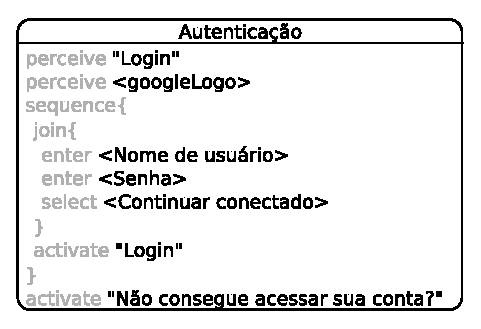
\includegraphics[scale=1.000]{images/login-web-is.eps}
%      \label{fig:espaco-de-interacao-a}
%    } 
%    \quad
%    \subfigure[Formulário web]{
%      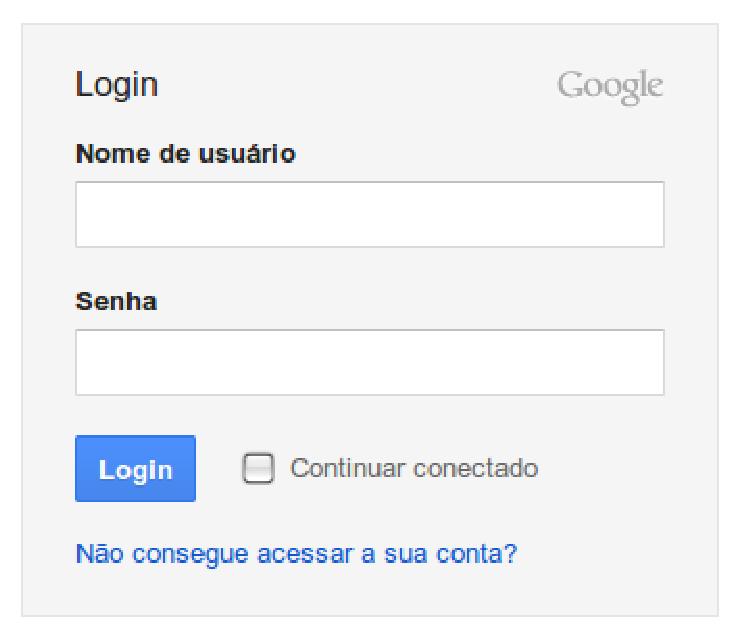
\includegraphics[scale=0.500]{images/login-web.eps}
%      \label{fig:espaco-de-interacao-b}
%    }
%
%    \caption{Exemplo  de  um  espaço  de  interação  representando  um
%      formulário web.}
%
%    \label{fig:espaco-de-interacao}
%  \end{center}
%\end{figure}
%
%O  espaço   de  interação  da  figura~\ref{fig:espaco-de-interacao-a},
%expressa a  seguinte semântica  ou intenção comunicativa  do designer:
%``aqui/agora você pode  efetuar o {\em Login} na  aplicação, para isso
%você deverá primeiro fornecer pelo menos as informações para {\em Nome
%  do usuário} e {\em Senha},  depois ativar o {\em Login} para acionar
%a  função da  aplicação  correspondente.  Se  houver  interesse que  o
%sistema  mantenha  suas  informações  para  uso  em  sessões  futuras,
%selecione  {\em Continuar  conectado},  antes de  ativar {\em  Login}.
%Caso tenha problemas  na autenticação, ative o link  {\em Não consegue
%  acessar sua conta?}  para mais informações''. Dito de outra forma, o
%que  ele quer  que seja  comunicado ao  usuário, através  da interface
%naquele ponto do processo de interação.  Em resumo, {\em o que} e {\em
%  como} o usuário deve agir para usufruir dessa funcionalidade.
%
%Concretamente,  tem-se  como  exemplo  uma janela,  em  uma  interface
%gráfica, ou um formulário, em uma página Web, onde existem vários {\em
%  widgets}  usados pelo  usuário para  entrar com  os dados,  ativar a
%execução da funcionalidade  correspondente e visualizar os resultados.
%Como  visto, os  {\em  widgets}  para entrada  de  dados, ativação  de
%processos e  visualização dos resultados são  representados pelas {\em
%  interações  básicas}.  Na  figura~\ref{fig:espaco-de-interacao-b}, é
%possível  perceber  um   formulário  associado  a  uma  funcionalidade
%específica oferecida pelo sistema, com seus respectivos {\em widgets},
%para o usuário comandar aquela funcionalidade.
%
%Como já  dito, em geral,  um espaço de  interação está ligado,  a pelo
%menos,  uma   função  da  aplicação,   que  deve  ser   sua  principal
%funcionalidade.  Isso pode confundir o leitor levando-o a imaginar que
%um  espaço  de interação  permite  ao  usuário  comandar mais  de  uma
%funcionalidade da aplicação. Em termos de objetividade, não é isso que
%ocorre.   Contudo,  em  muitas  situações, a  interface  realiza,  por
%exemplo, diversas  consultas ao sistema,  principalmente para produzir
%listas  de  faixa de  valores  a serem  usados  pelo  usuário para  se
%produzir as informações necessárias  à execução da função da aplicação
%principal.
%
%Para exemplificar  tal situação, tem-se  uma interface onde  o usuário
%deve  selecionar uma cidade  para indicar  seu endereço,  porém, antes
%deve selecionar o  estado, fazendo com que a  ativação de uma consulta
%seja realizada pelo sistema e  a lista de cidades seja disponibilizada
%na  interface para posterior  seleção do  usuário. Outro  exemplo, bem
%comum atualmente,  são as  aplicações Web, com  suporte a  campos {\em
%  autocomplete}, que  realizam consultas  ao sistema a  cada caractere
%digitado naquele  campo e  produzem uma lista  de sugestão  de valores
%para que o usuário possa selecionar aquele que lhe interessar, sem ter
%que completar a digitação.
%
%Para  mostrar como  o designer  pode usar  \aladim\ para  modelar essa
%situação,      pode      se       observar      o      exemplo      da
%figura~\ref{fig:IncluirCliente}.   Como as  transições  são provocadas
%sempre  por uma  interação  básica  dentro do  espaço  de interação  é
%possível perceber que, quando a interação básica ``select <estado>'' é
%executada,  ocorre a  transição  de ativação  da  função da  aplicação
%``consultaCidades''. Após a execução  do processo, sua transição é uma
%reação de  sucesso, com  uma lista de  cidades associada  à informação
%<cidade>,  para  o espaço  de  interação,  no  qual o  usuário  poderá
%continuar  no processo  de interação  e selecionar  uma  cidade dentre
%aquelas  listadas  para  o  estado  selecionado  na  interação  básica
%anterior.
%
%\figura{Espaço de interação com múltiplas funções da aplicação.}
%       {fig:IncluirCliente}
%       {incluir-cliente.eps}
%       {0.950}
%       {0}
%
%É  importante ressaltar que  numa perspectiva  comunicativa e  com uma
%preocupação  na   escolha  de  signos   que  mantenham  o   mínimo  de
%consistência  dentro do modelo,  sugere-se que  a principal  função da
%aplicação que estabelece a motivação de se interagir com aquele espaço
%de interação, apresente-se estritamente relacionada à identificação do
%espaço  de  interação.   Essa   preocupação  acontece  no  exemplo  da
%figura~\ref{fig:IncluirCliente},  onde  o  espaço  de  interação  está
%associada   às    funções   de   aplicação    ``consultarCidades''   e
%``incluirCliente''. Nela  é possível  observar que essa  última função
%possui a mesma identificação que  o espaço de interação.  Isso permite
%que não se levante  dúvida sobre qual é a função principal  e qual é a
%secundária,  usada  para auxiliar  o  usuário  no processo  interativo
%necessário para comandar a função principal.
%
%A modelagem da  interação do usuário com o  sistema, usando \aladim, é
%guiado  pelo diagrama de  casos de  uso, o  que torna  possível ter-se
%apenas  um modelo  para  uma  aplicação modesta  com  poucos casos  de
%uso. Contudo,  é comum que se  tenha aplicações com  elevado número de
%casos  de  uso,  de  maneira  que  produzir e  ler  apenas  um  modelo
%\aladim\ para todos os casos de uso pode ser frustante.
%
%Diante disso, é  possível construir um modelo \aladim\  para cada caso
%de  uso  ou  até  um  conjunto  deles.   Contudo,  para  se  manter  a
%consistência  do modelo  como  um  todo, é  necessário  se garantir  a
%rastreabilidade das transições  possíveis entre os respectivos espaços
%de interação,  definidos ao longo dos  vários modelos de  cada caso de
%uso. Portanto, ao  se modelar a interação para  um determinado caso de
%uso, é  possível identificar a  necessidade de referenciar  espaços de
%interações presentes  ou definidos em  modelos de interação  de outros
%casos de uso.
%
%Com    o     exemplo    dessa    situação     pode-se    observar    a
%figura~\ref{fig:ReferenceInteractionSpace},  cujo modelo  de interação
%para um caso de uso  de ``Escrever mensagem'', apresenta a intenção do
%designer em comunicar:  (a) que o processo de  interação inicia-se com
%uma transição vinda de um  espaço de interação definido noutro modelo,
%de outro  caso de  uso e  que foi provocada  por uma  interação básica
%identificada (naquele espaço de interação) por ``escrever''; (b) que a
%interação usuário-sistema  se dará através  de um espaço  de interação
%para  o  usuário  produzir  as informações  necessárias,  ativação  da
%funcionalidade  correspondente,  incluindo  situações  de  exceção  na
%execução e a  desistência por parte do usuário; (c)  que no sucesso do
%envio da mensagem, ou na  desistência do usuário de postar a mensagem,
%o  processo de interação  se encerrará  com as  respectivas transições
%para o espaço de interação ``Examinar mensagens''.
%
%\figura{Exemplo de referência para um espaço de interação.}
%       {fig:ReferenceInteractionSpace}
%       {ReferencelInteractionSpace.eps}
%       {0.850}
%       {0}
%
%Isso permite dizer que, apesar da fragmentação do modelo de interação,
%é  possível  se  manter   a  rastreabilidade  sobre  os  artefatos,  e
%principalmente, a consistência na  representação do processo global de
%interação.  Isto  é, mesmo modelando a  interação para um  caso de uso
%específico,  busca-se facilitar a  identificação da  seguinte situação
%dentro do  processo de interação: ``de  onde o usuário  veio, antes de
%chegar naquele ponto do processo de  interação, o que ele pode fazer e
%como fazê-lo e para onde ele irá a partir daquele ponto''.
%
%Na   figura~\ref{fig:ReferenceInteractionSpace},    no   contexto   de
%``Escrever mensagem'', é possível  reconhecer que o fluxo de interação
%veio do  espaço de interação ``Examinar  mensagens'', detalhado noutro
%contexto,  e  irá voltar  para  o mesmo,  logo  após  a execução,  com
%sucesso,   da  função   de  aplicação   ``enviarMensagem'',   ou  pela
%desistência do envio por parte do usuário.
%
%Existem ainda situações  em que a aplicação sendo  modelada permite ou
%exige  que o  usuário interaja  com  outra aplicação.   Nesse caso,  o
%processo  de interação  irá ocorrer  dentro dos  espaços  de interação
%daquela  aplicação, que  por  sua  vez não  estão  sendo modelados  e,
%portanto, são desconhecidos.  Assim,  o processo de interação modelado
%irá transitar  para um espaço de interação  especial, representado por
%um  retângulo  de  cantos  arredondados com  apenas  um  compartimento
%contendo o nome da aplicação  e terá suas bordas desenhadas com linhas
%tracejadas,               como               ilustrado              na
%figura~\ref{fig:ExternalInteractionSpace}.
%
%\figura{Exemplo de um espaço de interação externo à aplicação.}
%       {fig:ExternalInteractionSpace}
%       {ExternalInteractionSpace.eps}
%       {0.750}
%       {0}
%
%%=====================================================================
%\subsection{Função da aplicação}
%\label{applicationFunctions}
%%=====================================================================
%
%Uma {\em função da aplicação} é usada para representar onde e quando o
%sistema   irá  atuar  no   processo  de   interação,  especificamente,
%executando um  processo que realiza  alguma das regras (ou  lógica) de
%negócio da aplicação, ou seja,  os serviços que a aplicação oferece ao
%usuário  para ele  realizar  suas tarefas.   Uma  função da  aplicação
%poderá produzir novas informações  e retornar aos espaços de interação
%para informar o usuário dos resultados do processo.  São representadas
%por retângulos  com dois compartimentos,  sendo o primeiro  usado para
%sua identificação e o  segundo reservado para alguma possível expansão
%futura.     Uma    função   da    aplicação    é   exemplificada    na
%figura~\ref{fig:ApplicationFunction}.
%
%\figura{Exemplo de função da aplicação.}
%       {fig:ApplicationFunction}
%       {application-function.eps}
%       {0.750}
%       {0}
%
%Como todo  processo computacional, as funções da  aplicação consomem e
%produzem informações  quando são  executadas pelo sistema,  contudo, a
%especificação das  funcionalidades da aplicação,  como se faz  na \es,
%não  é  endereçada  em  \aladim\.   O designer,  como  já  dito,  está
%preocupado em  modelar {\em o que}  o usuário pode fazer  e {\em como}
%ele deve agir para  usufruir do sistema e não em modelar  {em o que} o
%sistema faz e {\em como} se comporta para atender ao usuário.
%
%Dessa forma, alguns desses aspectos sobre a função da aplicação já são
%cobertos  no modelo,  sem os  rigores da  \es, através  das interações
%básicas  postas  nos respectivos  espaços  de  interação associados  à
%função da aplicação; de maneira  que as informações que esta necessita
%e  produz  sejam,  respectivamente,  fornecidas e  percebidas,  nesses
%espaços        de       interação,       vide        exemplos       da
%figuras~\ref{fig:interaction-space-all}.    Além   disso,  mesmo   não
%endereçando  seus mecanismos  de  controle interno  como suspensão  ou
%interrupção,  por exemplo, \aladim\  permite modelar  o que  o usuário
%precisa  fazer  para  controlar  a  execução  também  nos  espaços  de
%interação, através  das respectivas interações básicas,  como pode ser
%observado no exemplo da figura~\ref{fig:copy-files}.
%
%Também  é  importante  destacar   que  as  funções  da  aplicação  são
%abstrações  para   as  funcionalidades  oferecidas   pelo  sistema,  e
%consequente,  também estão  associadas  aos casos  de uso,  levantados
%durante a análise dos requisitos da aplicação. Portanto, se o designer
%estiver modelando  a interação num  único modelo diagrama,  ele deverá
%possuir no mínimo uma função de aplicação para cada caso de uso.
%
%%=====================================================================
%\subsection{Transições}
%\label{transitions}
%%=====================================================================
%
%Para comunicar onde e quando se darão as mudanças de quem irá atuar no
%processo  de   interação,  deve-se  usar  uma   {\em  transição}.   As
%transições de um  espaço de interação para outro  podem ser disparadas
%por  qualquer  interação  básica  dentro  do espaço  de  interação  de
%origem. Cada  uma delas deve ser  representada por uma  linha sólida e
%possuir,  como rótulo,  o nome  da  interação básica  que a  disparou.
%Outra possibilidade é  por inatividade do usuário, nesse  caso, a seta
%deverá possuir rótulo com um valor temporal (ex.  50s, 3min) indicando
%que  após aquele  tempo de  inatividade  do usuário,  a transição  irá
%ocorrer.
%
%Existem duas  situações de transição  entre espaços de  interação.  Na
%primeira  não há  demanda  por funcionalidade  da  aplicação, isto  é,
%tem-se  apenas uma  {\em  navegação}.  Nesse caso  não  há mudança  da
%atuação do usuário para o  sistema, apenas que o usuário poderá/deverá
%continuar atuando em outro espaço de interação.  Essa situação é comum
%em espaços de interação que concentram chamadas a outros espaços, como
%janela com menus, por exemplo. A segunda é quando a transição demandar
%a execução de uma função da aplicação, sendo tratada de duas maneiras.
%
%Quando partir do espaço de  interação para a função da aplicação, onde
%é   considerada  uma   {\em  ação}   do  usuário   solicitando  alguma
%funcionalidade do sistema, deve ser representada por uma linha sólida.
%Quando  a transição  parte da  função da  aplicação para  o  espaço de
%interação,  é  considerada uma  {\em  reação}  do  sistema à  ação  do
%usuário, podendo ser representada de duas formas: (a) se a execução da
%função  da aplicação  terminar normalmente  será representada  por uma
%linha sólida, cujo rótulo  poderá ser alguma informação retornada pela
%função ou  uma mensagem explícita do  designer para o  usuário; (b) no
%caso da execução terminar de maneira anormal, a linha será tracejada e
%seu rótulo poderá ser alguma  indicação do motivo da falha, através de
%uma mensagem  explícita do designer e/ou alguma  informação do domínio
%ou      da      aplicação,      como     podemos      observar      na
%figura~\ref{fig:interaction-space-all}.
%
%\figura{Exemplo de um espaço de interação e função da aplicação.}
%       {fig:interaction-space-all}
%       {calculating-value-all.eps}
%       {0.700}
%       {0}
%
%As transições são usadas para indicar uma mudança do fluxo de ações do
%usuário para  o fluxo  de reações do  sistema.  Ainda  nesse contexto,
%existem  situações especiais em  que o  usuário poderá  realizar novas
%interações  básicas enquanto aguarda  uma reação  do sistema  para uma
%ação já  executada.  Nesse caso, o  espaço de interação  deve estar em
%``sincronismo''   com  a   função  da   aplicação.   Esta   ligação  é
%representada  por  setas  de   duplo  sentido.   Elas  são  destinadas
%exclusivamente para  representar uma ligação síncrona  entre um espaço
%de  interação e  uma  função da  aplicação.   Isto é,  mesmo quando  o
%processo  está em execução,  o usuário  poderá observar  seu progresso
%e/ou  intervir sobre o  mesmo.  Nesse  caso, a  seta não  deve possuir
%rótulo, como exemplificado na figura \ref{fig:copy-files}, onde depois
%de ter iniciado  o processo em {\em Copiar  arquivos}, o usuário, além
%de acompanhar o seu progresso, poderá suspender, reiniciar ou cancelar
%o processo em {\em Copiando arquivos}.
%
%\figura{Modelo para um cenário para cópia de arquivos.}
%       {fig:copy-files}
%       {copy-files.eps}
%       {0.650}
%       {0}
%
%%=====================================================================
%\section{Construindo um modelo completo}
%\label{aladimExamples}
%%=====================================================================
%
%Nesta  seção, é  apresentado um  exemplo de  como se  construir modelo
%completo, mesmo  que de tamanho limitado, usando  a linguagem \aladim,
%mostrando  principalmente  como   identificar  as  porções  do  modelo
%associadas aos casos  de uso da aplicação. Nesse  exemplo, trata-se de
%um modesto  sistema de correio  eletrônico, com um número  restrito de
%funcionalidades,  cujos requisitos  são especificados  no  diagrama de
%casos  de  uso  apresentado na  figura~\ref{fig:Email:System:Usecase},
%construída   usando    uma   versão   grátis    da   ferramenta   {\em
%  astah}\footnote{http://astah.net/editions/uml}.     O    modelo   de
%interação  correspondente,  na  linguagem  \aladim, é  apresentado  no
%diagrama da figura~\ref{fig:Email:System:Aladim}.
%
%\figura{Diagrama de casos de uso para um sistema 
%  de correio eletrônico.}
%       {fig:Email:System:Usecase}
%       {email-system-uc.eps}
%       {0.650}
%       {0}
%
%Na    figura~\ref{fig:Email:System:Aladim},    pode-se   observar    a
%correspondência  unitária  entre os  casos  de  uso  e os  espaços  de
%interação.  Isso  está ligado  ao fato de  um espaço de  interação ser
%usado para comunicar todo o conjunto de interações básicas necessárias
%para se usufruir  de determinada funcionalidade da aplicação,  o que é
%identificado   como  um  requisito   funcional  e   representado  pelo
%respectivo  caso  de uso.   Outra  importante  observação  é quanto  à
%visualização  dos anexos das  mensagens, que  não será  realizada pela
%própria  aplicação e sim  pelo visualizador  de arquivos,  definido no
%sistema operacional,  o que foi  modelado como uma referência  para um
%espaço de interação definido numa aplicação externa.
%
%\figura{Modelo \aladim\ correspondente ao diagrama de 
%  casos de uso da figura~\ref{fig:Email:System:Usecase}.}
%       {fig:Email:System:Aladim}
%       {email-system.eps}
%       {0.525}
%       {-90}
%
%A  figura~\ref{fig:Email:System:Aladim}, traz  um modelo  de interação
%para um sistema simples  de correio eletrônico, cujos requisitos estão
%especificados     no     diagrama     de     caso    de     uso     da
%figura~\ref{fig:Email:System:Usecase}.   Sendo que  para cada  caso de
%uso,  com  duas  exceções,  foi  modelado um  espaço  de  interação  e
%associado  a ele  uma  função da  aplicação  representando o  processo
%computacional responsável pela realização do caso de uso.
%
%A primeira  exceção foi do caso  de uso {\em Efetuar  logout}, que não
%precisou  de um  espaço de  interação para  isso, bastando  apenas uma
%interação básica  no espaço de  interação {\em Examinar  mensagens}. A
%outra  exceção foi  do caso  de uso  {\em Visualizar  anexos},  que na
%verdade, foi modelado com uma referência para uma aplicação externa ao
%sistema sendo desenvolvido.
%
%%=====================================================================
%\section{Considerações sobre o capítulo}
%\label{aladimSynthesis}
%%=====================================================================
%
%\aladim\  foi  concebida para  auxiliar  o  designer,  não só  na  sua
%comunicação com o usuário por meio da interface, mas também com aquele
%que  antecede  e  atua  como  um tradutor  para  essa  comunicação,  o
%desenvolvedor. Dessa forma, neste trabalho, o design da interação como
%proposto no ciclo  de vida da figura~\ref{fig:Design:Lifecycle:Model},
%considera  que   o  primeiro  estágio  desse   ciclo,  que  compreende
%principalmente os requisitos, será finalizado com um diagrama de casos
%de uso.   A partir desse diagrama é  que o designer irá  lançar mão de
%\aladim\ para  modelar o processo  de interação necessário para  que o
%usuário possa  fazer uso das funcionalidades  oferecidas pelo sistema,
%representadas  no  diagrama  de   casos  de  uso  como  requisitos  da
%aplicação.
%
%Como já visto, \aladim\ se baseia  na \se\ para auxiliar o designer no
%processo comunicativo com o usuário.   Isso é possível através de seus
%elementos,  conceitualmente  definidos de  maneira  que seja  possível
%modelar  e  refletir  sobre  a  interação, estruturando  o  modelo  de
%interação  como  uma  mensagem   interativa  que  comunica  a  própria
%interação.  Dessa forma, a estrutura da mensagem interativa é composta
%por  {\em espaços  de  interação},  que comandam  a  execução de  {\em
%  funções  da  aplicação}.   Os  comandos  ocorrem  através  das  {\em
%  interações básicas},  que permitirão ao usuário  produzir e consumir
%as informações  necessárias à  execução da funcionalidade  em questão,
%bem como acionar sua execução.   Cada espaço de interação poderá estar
%organizado  por meio  dos {\em  operadores}, que  permitem estabelecer
%vários tipos  de relacionamentos entre as interações  básicas; o fluxo
%de interação entre os vários espaços de interação, bem como destes com
%as funções de aplicação, é comunicado através das {\em transições}.
%
%Como demostrado na definição dos elementos da linguagem, o embasamento
%na \se\ se fez necessário pela preocupação com o aspecto comunicativo,
%tanto  da linguagem  em  si,  quanto do  produto  final resultante,  o
%sistema  interativo. Cada  elemento de  \aladim\ possui  esse aspecto,
%isto  é,  se  constitui  como  um  signo que  irá  compor  a  mensagem
%estruturada  do  design  sobre  o  diálogo entre  usuário  e  sistema,
%comunicando quais  as ações que  o usuário pode/deve executar  e quais
%reações esperar do sistema, em resumo, o modelo de interação.
%
%%%% Local Variables: 
%%%% mode: latex
%%%% TeX-master: "main"
%%%% End: 
		% Linguagem para modelar a interação
%%%=====================================================================
%\chapter{Ferramenta para modelagem \aladim}
%\label{editor}
%%=====================================================================
%
%Como já  dito, os elementos  da linguagem \aladim\ foram  definidos de
%acordo  com  a  \se~\cite{deSouza:2005},  o  ciclo  de  design  usando
%\aladim\ segue aquele  proposto por \citeonline{Sharp:etal:2007} e que
%o desenvolvimento da ferramenta para modelagem empregou os padrões que
%compõem  a  abordagem  \mda~\cite{OMG:MDA:2001}.   Dessa  forma,  este
%capítulo apresenta o  {\em Editor \aladim} e descreve  como se deu seu
%desenvolvimento.
%
%%=====================================================================
%\section{Requisitos da ferramenta}
%\label{aladimEditor}
%%=====================================================================
%
%Como  visto na  seção~\ref{generalVision},  \aladim\ possui  elementos
%diagramáticos  e  textuais.    Contudo,  independente  se  textual  ou
%diagramático,  o suporte  ferramental para  auxiliar na  utilização de
%determinada linguagem, sempre foi visto como um importante diferencial
%para seus  usuários.  Seguindo esta perspectiva,  foi desenvolvida uma
%ferramenta de suporte à linguagem, o {\em Editor \aladim}.  Para isso,
%o  primeiro passo  foi especificar  um  conjunto de  requisitos que  a
%ferramenta deveria atender.  Tais requisitos são listados a seguir:
%
%\begin{enumerate}
% 
% \item  {\em Permitir a  edição de  diagramas}: A  ferramenta deveria
%    permitir ao designer a construção de modelos de maneira intuitiva,
%    muito semelhante aos editores  gráficos mais comuns, empregado uma
%    área de  edição e uma  paleta de elementos da  linguagem. Bastando
%    arrastar os componentes do diagrama da paleta para área de edição.
%
%  \item  {\em  Suportar   uma  notação  processável}:  Considerando  a
%    possibilidade de  um modelo  \aladim\ ser empregado  em processos,
%    como a  geração automática de  interface, por exemplo.   Até mesmo
%    para auxiliar no próximo requisito.
%
%  \item  {\em   Validar  sintaticamente  o   diagrama}:  As  vantagens
%    esperadas   pelo   suporte   de   um   editor   gráfico,   estarão
%    comprometidas, se  o designer tiver  um esforço muito  grande para
%    checar visual e mentalmente se seu diagrama está correto. Assim, é
%    imprescindível que a ferramenta garanta ao designer que o diagrama
%    que ele está construindo esteja sintaticamente correto.
%
%\end{enumerate}
%
%Buscando   atender  aos   requisitos   estabelecidos,  optou-se   pelo
%desenvolvimento  da   ferramenta  sob  a   forma  de  plugin   para  o
%Eclipse\footnote{http://www.eclipse.org},  que  é  uma  plataforma  de
%desenvolvimento  que  fornece uma  gama  de  serviços,  dentre eles  a
%criação de  plugins que podem ser carregados,  integrados e executados
%dentro do  próprio ambiente.   A plataforma, tecnologias  e atividades
%desenvolvidas  para  criação do  Editor  \aladim\  são apresentados  a
%seguir.
%
%%=====================================================================
%\section{Tecnologias utilizadas}
%\label{editorEclipse}
%%=====================================================================
%
%A Fundação Eclipse possui vários projetos, onde são criadas e mantidas
%várias  ferramentas  integradas. Dentre  os  vários  projetos, o  {\em
%  Eclipse Modeling Project}\footnote{http://www.eclipse.org/modeling/}
%tem  o foco  na evolução  e promoção  das técnicas  de desenvolvimento
%baseado em  modelos, dentro da  comunidade de usuários  da plataforma.
%Para isso, ele provê  um conjunto unificado de frameworks, ferramentas
%e padrões de implementações~\cite{Steinberg:etal:2008}.
%
%O  \emf~({\em \Emf})~\cite{Budinsky:etal:2003}  é  a base  tecnológica
%para o {\em projeto modeling}, ele oferece toda infraestrutura para se
%metamodelar,  instanciar  e   manipular  modelos.   A  linguagem  para
%definição de metamodelos no \emf\ é  chamada de {\em Ecore}, que é uma
%implementação  para um subconjunto  do \mof.   O \emf\  possibilita ao
%usuário  gerar, a partir  de algum  modelo Ecore,  código java  (sob a
%forma de plugins  para a própria plataforma) que  irão possibilitar ao
%usuário  a criação  e manipulação  de  modelos em  conformidade com  o
%metamodelo  estabelecido,  possibilitando  inclusive  a  validação  do
%mesmo.
%
%No  \emf\ não  há necessidade  de uma  metodologia específica  para se
%definir o  metamodelo, pois, ele gera automaticamente  modelos Ecore a
%partir de uma série de fontes como por exemplo, um diagrama \uml~({\em
%  \Uml}), arquivos \xml~({\em \Xml})  e código java anotado.  Contudo,
%o suporte para criação e  manipulação, oferecida é feito por no máximo
%um  editor de  árvore,  onde  os elementos  do  modelo são  incluídos,
%manipulados e removidos, sob a forma de nós filhos e irmão ao longo da
%árvore.
%
%Já o \gef~({\em \Gef})~\cite{Majewski:2004} é um framework que permite
%a criação de  editores gráficos na plataforma, através  de definição e
%customização  dos  elementos que  irá  compor  o  diagrama, tais  como
%figuras,  nós,  nós filhos,  arestas  e  compartimentos.  Os  editores
%criados também são  incorporados à plataforma sob a  forma de plugins.
%Contudo, o \gef\ oferece  suporte apenas à representação dos elementos
%gráficos, deixando todo o controle do modelo por trás do diagrama, sob
%o controle do usuário.  Durante  muito tempo isso foi feito através de
%\pojo~({\em \Pojo}),  ou seja,  toda essa implementação  precisava ser
%feita de maneira manual.
%
%É nesse contexto que  surge o \gmf~\cite{Plante:2006} para facilitar a
%integração desses dois frameworks (\emf\ e \gef).  Assim é possível ao
%usuário   desenvolver   um  completo   editor   gráfico,  através   da
%especificação  de  quatro  modelos:   de  domínio,  de  definição  dos
%elementos  gráficos,  de  definição  da  paleta de  ferramentas  e  de
%mapeamento    entre   os   outros    modelos,   como    ilustrado   na
%figura~\ref{fig:GMF:Workflow}.   O modelo  de  domínio corresponde  ao
%metamodelo  que  será  usado  para  instanciar  os  modelos  que  irão
%alimentar a visão ou diagrama  \gef, no caso da linguagem \aladim, seu
%metamodelo será apresentado na seção~\ref{aladimMetamodel}, a seguir.
%
%\figura{Fluxo     de    atividades     do     \gmf,    extraído     de
%  \citeonline{Plante:2006}.}
%       {fig:GMF:Workflow}
%       {gmf-workflow.eps}
%       {0.500}
%       {0}
%
%Dessa forma, para o desenvolvimento  do {\em Editor \aladim}, usando o
%{\em Eclipse Modeling}, o principal  recurso usado foi \gmf\ que, como
%visto,   é   responsável   por   prover  componentes   generativos   e
%infraestrutura de tempo de execução para o desenvolvimento de editores
%gráficos baseados  no \emf\  e usando o  \gef. Integrando todos  sob a
%forma de plugins que podem ser integrados à própria plataforma.
%
%%=====================================================================
%\section{Metamodelo da linguagem}
%\label{aladimMetamodel}
%%=====================================================================
%
%Entre  as seções  \ref{basicInteractions}  e \ref{transitions},  foram
%apresentados, informalmente  (não processável), a  sintaxe e semântica
%dos  elementos  da  linguagem   \aladim.   Agora,  nesta  seção,  será
%apresentada o  metamodelo (processável) da  linguagem, especificando a
%sintaxe  e semântica  de seus  elementos.  Considerando  os requisitos
%estabelecidos  para  a  ferramenta  e  as  tecnologias  utilizadas,  o
%metamodelo é  especificado usando um  modelo, que é a  linguagem usada
%para  representar  modelos  no  \emf,  isto é,  metamodelos.   Como  a
%linguagem de modelagem Ecore é  especificada no \emf, o Ecore se torna
%um metamodelo de si mesmo~\cite{Budinsky:etal:2003}.
%
%Um modelo  Ecore pode ser  criado de várias  formas no \emf,  como por
%exemplo, a importação de diagramas \uml, \xml\ e código java anotação.
%A forma mais básica de manipulação  é através de um editor de árvores.
%Adicionalmente  é  possível  manipular  um  modelo  Ecore  de  maneira
%diagramática, sendo  que essa  forma foi utilizada  para a  criação do
%metamodelo  da  linguagem  \aladim,  cuja  representação  é  feita  na
%figura~\ref{fig:aladim:metamodel}.
%
%\figura{Metamodelo da linguagem \aladim.}
%       {fig:aladim:metamodel}
%       {aladim-metamodel.eps}
%       {0.750}
%       {0}
%
%Um {\em modelo de interação} é composto por dois conjuntos, um de {\em
%  elementos}  e  outro das  {\em  transições}  entre esses  elementos.
%Dessa  forma,  são necessários  pelo  menos  dois  elementos para  uma
%transição.  Um elemento é uma abstração para {\em função da aplicação}
%e  {\em  espaços},  que  é   outra  abstração  para  {\em  espaços  de
%  interação}, {\em pontos iniciais} e  {\em finais} para a interação e
%{\em espaços de interação referenciados} e {\em aplicações externas}.
%
%Um espaço de interação é composto por, pelo menos, uma {\em interação}
%que é uma abstração para {\em interações básicas} e {\em operadores de
%  interação}.  Os  operadores podem conter novas interações,  o que os
%tornam recursivos. Um  operador é uma abstração para  {\em join}, {\em
%  sequence}, {\em choose}, {\em  repeat} e {\em combine}.  Assim, como
%uma interação básica  é uma abstração para {\em  select}, {\em enter},
%{\em perceive} e {\em activate}.
%
%Uma transição é  uma abstração para {\em ação},  {\em navegação}, {\em
%  reação de sucesso}, {\em reação  de falha} e {\em sincronização}. As
%transições, quando  disparadas pelo usuário, devem  identificar o nome
%da informação  associada a interação  básica que disparou.   Já quando
%disparadas  pelas  funções  da  aplicação,  podem  levar  aos  espaços
%informações  sobre  resultados   ou  falhas  no  processamento.   Toda
%transição possui uma origem e um destino.
%
%O \emf\ oferece  suporte para a geração automática  de código capaz de
%editar  e  validar  um  modelo  de acordo  com  as  especificações  do
%metamodelo. A validação consiste, dentre outras coisas, na verificação
%de todas  as associações  estabelecidas no metamodelo,  incluindo suas
%cardinalidades.    Contudo,  algumas  situações   em  que   apenas  as
%associações, especializações e  cardinalidades não são suficiente para
%especificar   determinadas  restrições,  é   possível  fazer   uso  de
%\ocl~({\em  \Ocl}), que é  uma linguagem  formal usada  para descrever
%expressões em modelos~\cite{OMG:OCL:2012}.
%
%Como visto  na descrição das  transições (seção~\ref{transitions}), os
%diferentes  tipos de  transições têm  algumas  restrições específicas.
%Além  disso, o  metamodelo  da figura~\ref{fig:aladim:metamodel},  não
%especifica isso.  Dessa  forma, considerando que de acordo  com o tipo
%de transição,  as origens e  destinos devem ser de  tipos específicos,
%por  exemplo,  em uma  {\em  ação}  a origem  deve  ser  um espaço  de
%interação e  o destino uma  função da aplicação, essas  restrições são
%especificas   através  de  invariantes   definidos  nas   classes  que
%especializam as abstrações, usando  \ocl, que também são traduzidos em
%código  para validação  durante  a modelagem  usando  o editor.   Este
%invariantes são descritos a seguir:
%
%\begin{itemize}
%
%  \item {\em  Action}: Especialização de transição que  liga um espaço
%    de interação a uma função da aplicação:
%
%    \begin{itemize}
%
%      \item {\em  not self.source.oclIsTypeOf(ApplicationFunction)}: A
%        origem de uma ação não pode ser uma função da aplicação;
%
%      \item   {\em   self.target.oclIsTypeOf(ApplicationFunction)}:  O
%        destino uma ação deve ser uma função da aplicação;
%
%      \item   {\em  self.source.oclIsTypeOf(InteractionSpace)\\implies
%        self.source.oclAsType(InteractionSpace).getNestedBasicInteractions()\\->exists(i:
%        BasicInteraction  | i.information  = self.information)}:  Se a
%        origem de  uma ação for  um espaço de interação,  deve existir
%        uma interação básica em  seu interior responsável por disparar
%        a transição;
%
%    \end{itemize}
%
%  \item  {\em  Reaction}: Especialização  de  transição  que liga  uma
%    função da aplicação a um espaço de interação:
%
%    \begin{itemize}
%
%      \item   {\em   self.source.oclIsTypeOf(ApplicationFunction)}:  A
%        origem de uma reação deve ser uma função da aplicação;
%
%      \item {\em  not self.target.oclIsTypeOf(ApplicationFunction)}: O
%        destino de uma reação não pode ser uma função da aplicação;
%
%    \end{itemize}
%
%  \item  {\em Navigation}:  Especialização de  transição que  liga uma
%    função da aplicação a um espaço de interação:
%
%    \begin{itemize}
%
%      \item {\em  not self.source.oclIsTypeOf(ApplicationFunction)}: A
%        origem de uma navegação não pode ser uma função da aplicação;
%
%      \item {\em  not self.target.oclIsTypeOf(ApplicationFunction)}: O
%        destino de uma navegação não pode ser uma função da aplicação;
%
%      \item   {\em  self.source.oclIsTypeOf(InteractionSpace)\\implies
%        self.source.oclAsType(InteractionSpace).getNestedBasicInteractions()\\->exists(i:
%        BasicInteraction  | i.information  = self.information)}:  Se a
%        origem  de uma  navegação  for um  espaço  de interação,  deve
%        existir uma  interação básica em seu  interior responsável por
%        disparar a transição;
%
%    \end{itemize}
%
%  \item {\em Synchronization}: Especialização de transição que liga um
%    espaço de interação a uma função da aplicação:
%
%    \begin{itemize}
%
%      \item {\em  not self.source.oclIsTypeOf(ApplicationFunction)}: A
%        origem  de  uma  sincronização  não  pode ser  uma  função  da
%        aplicação;
%
%      \item   {\em   self.target.oclIsTypeOf(ApplicationFunction)}:  O
%        destino de uma sincronização deve ser uma função da aplicação;
%
%    \end{itemize}
%
%\end{itemize}
%
%Os resultados do processo de validação de um modelo \aladim, podem ser
%observados   na   figura~\ref{fig:aladim:editor},   através   de   uma
%janela/painel    específico    para    apresentação   dos    problemas
%ocorridos. Além disso,  os elementos do diagrama são  decorados com os
%indicadores desses problemas. No  caso apresentado na figura, os erros
%decorrem justamente pela  violação de algumas restrições especificadas
%nos {\em invariantes} descritos acima.
%
%%=====================================================================
%\section{Editor \aladim\ em execução}
%\label{editorRunning}
%%=====================================================================
%
%Como resultado,  de tudo que  foi descrito nas seções  anteriores, foi
%produzido o {\em Editor \aladim} que pode ser visualizado, em execução
%sob a  forma de  um plugin já  completamente integrado ao  Eclipse, na
%figura~\ref{fig:aladim:editor},  onde  os  componentes  principais  do
%editor,  distribuídos  sob a  forma  janelas  ou  painéis do  ambiente
%Eclipse, são descritos a seguir.
%
%A  primeira,  mais  à esquerda,  é  a  janela  do {\em  explorador  de
%  pacotes}, onde  ficam os projetos que empacotam  os diagramas.  Cada
%projeto é armazenado no sistema de arquivo sob a forma de uma pasta ou
%diretório. Já  os diagramas  são armazenados sob  a forma  de arquivo,
%sendo dois para cada diagrama.   Um arquivo ({\tt .aladim}) armazena o
%\xml\ do  modelo, isto  é as instâncias  dos elementos  do metamodelo,
%implementados usando o  \emf.  Outro arquivo ({\tt .aladim\_diagram}),
%armazena o \xml\ do diagrama,  isto é, os elementos visuais associados
%aos elementos do modelo, implementados usando o \gef.
%
%A  segunda janela, posicionada  ao centro,  é a  {\em área  de edição}
%propriamente  dita,  é nela  que  o  designer  desenha seus  diagramas
%\aladim.  Para  cada elemento  visual presente no  diagrama, desenhado
%através do \gef, o ambiente,  através do \gmf, persiste um elemento no
%modelo, com  auxilio do \emf.   As operações relacionadas  à aparência
%dos  elementos visuais  (cor, fonte,  posição, etc.)   são persistidas
%apenas  no  diagrama   (arquivo  .aladim\_diagram),  enquanto  que  as
%operações   conceituais,  como  adição   e/ou  remoção,   mudanças  de
%propriedades e  referências dos  elementos, são persistidas  no modelo
%(arquivo .aladim), sendo que o sincronismo entre esses dois arquivos é
%completamente garantido pelo \gmf.
%
%Na  janela  mais  à  direita  fica  a {\em  paleta}  de  elementos  da
%linguagem. No  estilo {\em drag-and-drop}, o  designer deve selecionar
%cada  elemento e  adicioná-los  ao diagrama,  sendo  editar na  região
%central. Os elementos da paleta estão organizados em cinco categorias,
%que se comprimem e se  expandem para apresentação dos elementos. Essas
%categorias são:
%
%\begin{itemize}
%
%  \item  {\em Geral}: Permite  adicionar os  elementos mais  gerais da
%    linguagem, como  espaço de interação  ou função da  aplicação, por
%    exemplo.
%
%  \item {\em  Operador}: Permite adicionar, a um  espaço de interação,
%    os operadores como junção ou escolha, por exemplo.
%
%  \item {\em Interação}: Permite adicionar as interações básicas, como
%    entre com uma informação ou selecione uma informação, por exemplo.
%
%  \item {\em Transição}: Permite  adicionar as transições, com ação ou
%    navegação, entre os elementos gerais da linguagem.
%
%\end{itemize}
%
%Na parte inferior ficam várias janelas, entre elas a de edição de {\em
%  propriedades}  para elementos  selecionados no  modelo e  a  de {\em
%  problemas}  encontrados  no  modelo  que  decorrem  do  processo  de
%validação      do     mesmo.       No     caso      apresentado     na
%figura~\ref{fig:aladim:editor},  são  apresentados  quatro  problemas,
%propositalmente deixados no modelo.   Observe que além da listagem dos
%problemas com a indicação do  tipo de problema e sua localização, eles
%também são assinalados no diagrama através de decoração adicionados ao
%componente visual corresponde  ao elemento do modelo, que  ao passar o
%mouse sobre ele irá informar o tipo de problema ocorrido.
%
%\figura{Editor \aladim\ em execução integrado ao Eclipse.}
%       {fig:aladim:editor}
%       {aladim-editor.eps}
%       {0.555}
%       {-90}
%
%%=====================================================================
%\section{Considerações sobre o capítulo}
%\label{editorSynthesis}
%%=====================================================================
%
%Este  capítulo  apresentou  o  {\em Editor  \aladim},  uma  ferramenta
%desenvolvida  para permitir  a construção  de  diagramas representando
%modelos  nessa  linguagem. Seu  objetivo  é  auxiliar  no processo  de
%comunicação   do  designer  com   os  demais   membro  da   equipe  de
%desenvolvimento, especialmente os desenvolvedores.
%
%Desenvolvido  usando a  abordagem  \mda\ e  concretizado como  plugins
%integrados ao Eclipse, a  ferramenta permite usar todas as facilidades
%oferecidas pela plataforma.  Além  disso, dentro da abordagem \mda, os
%modelos \aladim\  estão num  nível \pim\ de  abstração, o  que permite
%que, usando  o metamodelo de \aladim, possam  ser produzidos processos
%automáticos  para  os  demais  níveis.  Possibilitando,  inclusive,  a
%geração automática de código da interface para diversas plataformas.
%
%Tudo   isso  demonstra   que  a   ferramenta  atende   aos  requisitos
%(seção~\ref{aladimEditor}) para os quais ela foi desenvolvida. Além da
%edição,  no  estilo  {\em  drag-and-drop}, dos  diagramas  \aladim,  a
%ferramenta  também possui  um editor  independente, que  possibilita a
%edição do modelo como uma  árvore. Sendo que a ferramenta mantém esses
%dois   arquivos  sincronizados   e  quaisquer   alterações  em   um  é
%automaticamente refletida no outro.
%
%%%% Local Variables: 
%%%% mode: latex
%%%% TeX-master: "main"
%%%% End: 
		% Ferramenta para modelagem da interação
%%%=====================================================================
\chapter{Estendendo $\pi$-SOD-M para a plataforma WS-BPEL 2.0}
%%\label{Complementando $\pi$-SOD-M}
%%%=====================================================================
%%
Este capítulo descreve a extensão proposta para aumentar o número de  plataformas especificas do método $\pi$-SOD-M, abrangendo o desenvolvimento de sistemas orientados a serviços para a linguagem de orquestração WS-BPEL 2.0. A construção de aplicações com o método $\pi$-SOD-M inicia-se na modelagem de requisitos funcionais e não funcionais a partir de um modelo $\pi$-Use Case, em seguida estes casos de uso são transformados em uma serie de modelos PIM e PSM antes de finalmente gerar o código que implementa a aplicação.

O ambiente $\pi$-SOD-M foi construído através da IDE Eclipse, mais especificamente utilizando \textit{Eclipse Modelling Framework} (EMF) para gerar o meta-modelo WS-BPEL 2.0, este \textit{framework} fornece utilitários necessários para definir, editar e manipular modelos. Para automatizar as transformações entre modelos utilizamos a linguagem ATL, ao qual é suportada pela IDE Eclipse em sua suíte de desenvolvimento. $\pi$-SOD-M Utiliza este ambiente para gerar composições de serviços em $\pi$-PEWS \cite{Placido}. Após nossa extensão do método $\pi$-SOD-M também construirá composições de serviços em WS-BPEL2.0.

O restante deste capítulo está organizado da seguinte forma. Seção 4.1 descreve detalhadamente as entidades e suas funções da linguagem WS-BPEL 2.0. A seção 4.2 descreve como WS-BPEL 2.0 será incorporado ao metodologia $\pi$-SOD-M. Seção 4.3 descreve as alterações feitas para estender o ambiente $\pi$-SOD-M, para a adição de novos componentes para geração de especificação de sistemas em diferentes linguagens. Seção 4.4 descreve as transformações entre modelos citadas anteriormente. Seção 4.5 faz uma comparação entre códigos gerados pela metodologia $\pi$-SOD-M para as plataformas $\pi$-PEWS e WS-BPEL, e  por fim conclui capítulo.
%%%=====================================================================
\section{Meta-modelo WS-BPEL}%4.1
%%\label{cdn}
%%%=====================================================================


Em construção!!!


%%%%=====================================================================
\subsection{Web Services-Business Process Executation Language}
\label{WS-BPEL}
%%%%=====================================================================
\textit{Web Services-Business Process Execution Language} (WS-BPEL) é uma linguagem de composição com sintaxe baseada em XML, usada para descrever composição, orquestração, coordenação e processos de negócios composto por \textit{Web Services} (WS)\cite{BPEL20}. Assim como também, pode ser utilizada para criar serviços a partir da coordenação de outros serviços pré-existentes.

Um processo BPEL, descreve como ocorre o relacionamento entre diversos \textit{web services} participantes de uma composição. Para descrever tais relacionamentos, BPEL oferece determinados tipos de construções similares as das linguagens de programação tradicionalmente conhecidas, como por exemplo: estrutura de repetição, condicionais, variáveis e atribuição, tratamento de exceções, parceiros de negócio e a coordenação destes parceiros. 

Para que seja possível construir um processo de negócio BPEL é necessário uma série de elementos fundamentais para especificação de um processo de negócio. A estrutura básica de um processo BPEL é formada por três seções: \textit{PartnerLinks, Variables e Activities}. Desta maneira um esqueleto de um processo BPEL assemelha-se a um documento XML tradicional. A  listagem de código ilustra o esqueleto base de um processo descrito WS-BPEL.

\lstinputlisting[language=XML,caption={Esqueleto de um processo BPEL.},label=Esqueleto de um processo BPEL]{CodigosXML/esqueletoprocessoBPEL.xml}

A seguir descreveremos cada uma das seções demonstradas na listagem de código acima.

<partnerLinks>: Esta seção define os elementos responsáveis por definir o conjunto de parceiros de negócios (\textit{PartnerLink}) utilizados em uma descrição de processo BPEL, identificando desta maneira qual funcionalidade deve ser oferecida por cada serviço parceiro \cite{BPEL20}.

O elemento \textit{PartnerLink} ilustrado na \href{Esqueleto de um processo BPEL.}, estabelece um canal de comunicação direto entre os parceiros de serviço internos ou externos que atuam na execução de um processo BPEL. As ligações dos serviços parceiros (\textit{partner link}) devem estar associadas a um tipo de ligação entre parceiros (\textit{partner link type}) definidos na especificação do \textit{web services} no WSDL. Dependendo da necessidade da comunicação entre parceiros de serviços, o papel de um parceiro pode variar\cite{BPEL20}. 

Um parceiro de serviço pode ser invocado por um serviço do processo e atuar com o papel de provedor de serviços (\textit{service provider}). Entretanto, se o mesmo serviço do processo invoca um serviço diferente, ele atuará como solicitante de um serviço (\textit{service requesters}). A definição do papel de um \textit{partnerLink} é definida através dos atributos \textit{myRole} e \textit{partnerRole}, que estabelecem o papel de provedor de serviço ou serviço associado respectivamente. A listagem de código a seguir demonstra a sintaxe de uma atividade \textit{partnerLink} \cite{BPEL20}.

\lstinputlisting[language=XML,caption={Sintaxe da atividade patnerLink.}, label=PatnerLink]{CodigosXML/partnerLinks.xml}

<variables>: Esta seção define as variáveis dos dados usadas pelo processo de negócio, para manter  as mensagens que constituem uma parte do estado de um processo negócio. As mensagens que tem seu estado capturados pelas variáveis são na grande maioria das vezes as mensagens trocadas entre  os parceiros de negócio (\textit{patnerlink}). As definições são feitas em termos de tipos de mensagem WSDL, elementos ou tipos simples de esquemas XML \cite{BPEL20}. Elas são usadas para manter os dados de estado e o histórico do processo com base nas mensagens trocadas. 

As variáveis devem estar associadas a tipos de mensagens (\textit{menssages}) definidos na especificação WSDL. Variáveis podem conter dados que são necessários para a realização de estado relacionado com o processo e nunca trocada com parceiros. WS-BPEL usa três tipos de declarações de variáveis: tipo de mensagem WSDL, XML Schema tipo (simples ou complexa) e XML \textit{Schema} elemento. A listagem a segui demonstra a sintaxe da atividade <variables>.

\lstinputlisting[language=XML,caption={Sintaxe da atividade variables.}, label=variables]{CodigosXML/variables.xml}

<faultHandlers>: Esta seção é responsável por declarar todos os manipuladores de falhas do processo, os manipuladores de falha definem as atividades que devem ser executadas em resposta a falhas resultantes da invocação dos serviços de avaliação e aprovação. Em WS-BPEL, todas as falhas, seja ele interno ou resultantes de uma chamada de serviço, são identificados por um nome qualificado. Em particular, cada falha WSDL é identificada em WS-BPEL por um nome especifico formado pelo \textit{namespace} de destino do documento WSDL em que o tipo de porta relevante e o motivo da falha são definidos \cite{BPEL20}. A listagem a seguir demonstra a sintaxe de um <faultHandlers>.

\lstinputlisting[language=XML,caption={Sintaxe da atividade faultHandlers.}, label=faultHandlers]{CodigosXML/faultHandlers.xml}


\textit{activities}: Esta seção contém a descrição de todas as atividades que descrevem o comportamento geral do processo de negócio. O BPEL possui uma sintaxe com vários tipos de elementos, cuja conjunção consegue descrever todo o tipo de processo de negócio que um utilizador necessite. Assim como em qualquer outra linguagem de programação, a sintaxe da linguagem WS-BPEL, dispõe de primitivas básicas para declarar seus elementos em descrições de processos. Estas primitivas são chamadas de atividades\cite{BPEL20}. As atividades de um processo BPEL são dividas em duas categorias: as atividades básicas e atividades estruturadas. 

%%%=====================================================================
\subsubsection{Atividades Básicas}
%%\label{designSpace}
%%%=====================================================================

Atividades básicas são atividades simples que não exige nenhuma lógica mais elaborada que são responsáveis por descreverem os passos elementares do comportamento de um processo \cite{BPEL20}. Estas atividades são vistas como um componente que interage com algo externo ao processo, como por exemplo a invocação de um serviço externo ao processo através de uma de suas construções. 

Os comandos para definir uma atividade em uma descrição BPEL, são similares as \textit{tags} da linguagem XML, onde são denotados por um único caractere ASCII ou uma string de caracteres entre os sinais <(menor que) e (maior que)>, geralmente estes os comandos são denotados com palavras em inglês. Grande parte das \textit{tags} do BPEL, requerem seu fechamento. Então, tudo que estiver compreendido entre <comando> e </comando> será encarado como o corpo de um comando. A seguir descreveremos a semântica do conjunto de atividades básicas do padrão WS-BPEL 2.0. 

<invoke>: esta atividade é usada para chamar uma operação em um dado \textit{Web Services} oferecidos por prestadores de serviços a uma composição de serviços. Esta atividade pode incluir outras atividades básicas aninhadas, como manipulador de compensação e manipuladores de falhas. A listagem de código a seguir demonstra a sintaxe da atividade <invoke> \cite{BPEL20}.

\lstinputlisting[language=XML, caption={Sintaxe da atividade invoke.}, label=ConsWhile]{CodigosXML/invoke.xml}

<receive>: O elemento \textit{receive} permite que um serviço do processo permaneça em estado de espera, agindo como um prestador de serviço, enquanto o processo recebe um pedido de um parceiro de serviço externo. Esta atividade específica um \textit{PartnerLink} que contenha um \textit{myRole} usado para receber mensagens, o \textit{portType} (opcional) é a operação que espera que o parceiro invoca que \cite{BPEL20}. Este elemento possui um conjunto de atributos que atribui valores a uma comunicação esperada, são eles: 

\begin{itemize}

\item[•] \textit{partnerLink}: define o \textit{PartnerLink} correspondente, ao parceiro de serviço que esta participando da troca de mensagens do processo.

\item[•] \textit{portType}: define qual o parceiro de serviço que o processo espera receber uma mensagem de requisição.
 
\item[•] \textit{operation}: define a operação de um serviço que vai receber uma mensagem de um outro processo.

\item[•] \textit{variable}: define qual variável vai armazenar a mensagem de solicitação.

\item[•] \textit{createInstance}: este atributo é definido com um valor booleano, caso seja definido como "SIM", uma nova instancia do processo de troca de mensagem sera criada, para que seja possível receber os dados da ou das mensagens trocadas entre os vários parceiros do processo, caso seja definido como não o processo não poderá receber mensagens pois não haverá uma instancia de uma atividade para receber os dados da ou das mensagens trocadas entre os parceiros \cite{BPEL20}. A listagem a seguir demonstra a sintaxe da atividade <receive>.

\end{itemize}

\lstinputlisting[language=XML, caption={Sintaxe da atividade receive.}, label=ConsWhile]{CodigosXML/receive.xml}

Existem outras atividades básicas na linguagem WS-BPEL, estas são listadas a seguir:

\begin{itemize}


\item[•] <reply>: Esta atividade é usada para enviar uma resposta a um pedido previamente aceito através de uma mensagem da atividade <receive>. Uma atividade <reply> pode especificar um atributo variável que faz referência a variável que contém os dados da mensagem a ser enviada \cite{BPEL20} . A listagem a seguir demonstra a sintaxe da atividade <reply>.

%\lstinputlisting[language=XML]{reply.xml}

\item[•] <wait>: Esta atividade é especificada quando a necessidade de utilizar um temporizador para realiza uma pausa por um período de tempo ou data especificado é atingido. Se o período de tempo especificado for zero ou nulo então a atividade <Wait> é completada imediatamente \cite{BPEL20}.

%\lstinputlisting[language=XML]{wait.xml}

\item[•] <assign>: A atividade <assign> é utilizada para copiar dados de uma variável para outra, assim como também, para a construção de novas expressões e inserir dados utilizando expressões. O uso de expressões é motivado pela necessidade de realizar cálculos simples (como incrementar os números de sequência) \cite{BPEL20}. Expressões podem operar sobre variáveis, propriedades, constantes e literais para produzir um novo valor. A listagem a seguir demonstra a sintaxe da atividade <assign> .

%\lstinputlisting[language=XML]{assign.xml}

\item[•] <throw>: Esta atividade é utilizada quando um processo de negócio precisa sinalizar uma falha interna que ocorrera durante o seu fluxo de execução. A atividade <throw> fornece o nome para a falha, e pode, opcionalmente, fornecer dados com informações sobre a mesma. Um manipulador de falhas pode usar estes dados para lidar com a falha e para preencher quaisquer mensagens de falha que precisam ser enviados para outros serviços \cite{BPEL20}. A listagem a seguir demonstra a sintaxe da atividade <throw>.

%\lstinputlisting[language=XML]{throw.xml}

\item[•] <terminationHandler>:  A rescisão forçada de um escopo começa desativando manipuladores do escopo do evento e encerra a sua atividade principal e todas as instâncias de manipulador de funcionamento do evento. Depois disso, o <terminationHandler> personalizado para o âmbito de aplicação, se estiver presente, é executado. Caso contrário, o manipulador de encerramento padrão é executado \cite{BPEL20}. A listagem a seguir demonstra a sintaxe da atividade <terminationHandler>.

%\lstinputlisting[language=XML]{terminationHandler.xml}

\item[•] <compensate>: Esta atividade é usada para iniciar a compensação de falhas em todos os âmbitos internos que já tenham terminado a sua execução por completo com sucesso de modo padrão \cite{BPEL20}. A listagem a seguir demonstra a sintaxe da atividade <terminationHandler>.

%\lstinputlisting[language=XML]{compensate.xml}

\end{itemize}

Para construir atividades mais complexas ou estruturadas no padrão WS-BPEL 2.0 é preciso combinar as primitivas básicas com atividades de controle. 

%%%=====================================================================
\subsubsection{Atividades Estruturadas}
%%\label{designSpace}
%%%=====================================================================

As atividades estruturadas descrevem como um processo de negócio pode ser criado a partir da composição de atividades básicas. Compor atividades básicas permite que um processo expresse: fluxos de controle, tratamento de exceção, chamada a eventos externos ao processo, assim como também coordenar as trocas de mensagens entre as partes envolvidas em um processo de negócio \cite{BPEL20}.

É possível definir atividades estruturadas através de fluxos de controle. Um controle sequencial é fornecido pelas atividades <sequence>, <if>, <while>, <repeatUntil> e <forEach>. É possível também definir concorrência e sincronização entre atividades de um determinado processo, esta atividade estruturada é assegurada pela atividade <flow> e uma variação paralela da atividade <forEach>. A escolha de um serviço especifico por um evento interno ou externo ao processo em um fluxo também é possível através da atividade <pick>.

Em alguns casos é possível representar a semântica de uma atividade específica através da combinação de outras atividades, por exemplo, uma sequência pode ser descrita através da atividade <sequence>, entretanto a combinação da atividade de controle <flow> com atividades básicas como <receive> por exemplo definindo as ligações de um fluxo corretamente, é possível descrever sequências sem uso da atividade nativa <sequence>. Desta maneira é possível combinar atividades arbitrariamente para aumentar a expressividade da linguagem \cite{BPEL20}. A seguir descreveremos as atividades estruturadas do padrão WS-BEPL2.0.

<sequence>: A atividade <sequence> é responsável por expressar a sequencia de uma ou mais atividades em ordem léxica. Esta atividade só finaliza sua execução depois que a ultima atividade de seu escopo é executada. O código abaixo demonstra a sintaxe da atividade de controle <sequence> \cite{BPEL20}. A listagem a seguir demonstra a sintaxe da atividade <sequence>.

\lstinputlisting[language=XML, caption={Sintaxe da atividade sequence.}, label=sequence]{CodigosXML/sequence.xml}

<if>: A atividade de controle <if>, define um comportamento condicional para um fluxo a partir da avaliação de uma expressão booleana. É possível aninhar varias condições utilizando a atividade <if> ou o opcional <elseif>, seguidos por um elemento <else> opcional, que servirá como elemento default em caso de nenhuma das opções aninhadas serem avaliadas verdadeiramente. A partir da a avaliação verdadeira de uma expressão a atividade envolvida pelo escopo da atividade <if> é executada, caso contrario o elemento <else> ou <elseif> são executados em sequencia. Esta atividade de controle só termina quando as atividades executadas através das avaliações das expressões são encerradas, ou imediatamente quando uma <condição> não é avaliada como true e nenhum ramo <else> é especificado \cite{BPEL20}. A listagem a seguir demonstra a sintaxe da atividade <if>.

\lstinputlisting[language=XML, caption={Sintaxe da atividade if.}, label=if]{CodigosXML/if.xml}

<while>: Assim como nas linguagens de programação tradicionais a atividade <while> no BPEL 2.0 representa a repetição de uma ou mais atividades em seu escopo, onde a execução de uma iteração é executada após uma expressão booleana ser avaliada verdadeira. \cite{BPEL20}. A listagem a seguir demonstra a sintaxe da atividade <while>.

\lstinputlisting[language=XML, caption={sintaxe da atividade while.}, label=While]{CodigosXML/while.xml}

<repeatUntil>: Assim como <while>, a atividade de controle <repeatUntil> também representa uma execução repetida de uma ou mais atividades em seu escopo, esta repetição é executada ate que a avaliação de uma dada expressão booleana deixe de ser verdadeira, a avaliação da expressão booleana é feita depois de cada iteração desta atividade de controle, esta atividade é amplamente utilizada em situações que é necessária uma estrutura de controle que execute uma repetição pelo menos uma vez \cite{BPEL20}. A listagem a seguir demonstra a sintaxe da atividade <repeatUntil>.

\lstinputlisting[language=XML,caption={Sintaxe da atividade repeat until.}, label=repeatUntil]{CodigosXML/repeatUntil.xml}

<forEach>: A atividade <forEach> também pode executar varias atividades em paralelo, controlada por duas expressões <startCounterValue> e <finalCounterValue>, ao iniciar, esta atividade avalia estas duas expressões. Uma vez que estas expressões sejam avaliadas verdadeiramente, a atividade <forEach> irá executar sua atividade <scope> contida exatamente N+1 vezes, onde n é igual ao <finalCounterValue> menos o <startCounterValue>. Se essas expressões não retornam valores válidos, o processo BPEL: lança uma \textit{invalidExpressionValue}, e a atividade termina sua execução, ou caso o <startCounterValue> seja maior do que o <finalCounterValue>, a atividade <scope> não deve ser realizada e a atividade <forEach> está completa \cite{BPEL20}. A listagem a seguir demonstra a sintaxe da atividade <forEach>.

\lstinputlisting[language=XML, caption={Sintaxe da atividade forEach}, label=forEach]{CodigosXML/foreach.xml}

Existem outras atividades estruturadas na linguagem WS-BPEL, estas são listadas a seguir:

\begin{itemize}

\item[•] <pick>: Esta atividade de controle espera pela ocorrência de um evento específico em um conjunto de eventos, uma vez que este evento específico ocorre, imediatamente a atividade associada a este evento é executada. Uma vez que a atividade <pick> aceita um evento, ela não mais aceita eventos daquele conjunto de eventos. Esta atividade dispõe de um conjunto de ramos onde em cada um contendo uma associação evento-atividade \cite{BPEL20}. A atividade <pick> termina quando a atividade associada ao evento termina sua execução. 

%Esta atividade tem duas formas de aceitar eventos, os do tipo <onManssage> e os do tipo <onAlarm>. Os eventos do tipo <onManssage> assemelham-se a uma atividade <receive> no sentido de que aguardam pela recepção de uma mensagem de entrada. Já os eventos do tipo <onAlarm> tem uma semântica diferente, pois este tipo de evento são baseados em temporizadores onde a duração deve ser especificada através de duas clausulas, a clausula <for> especifica previamente a duração do evento em zero ou negativamente, e a clausula <until> especifica um prazo onde o tempo pode ser atingido ou ultrapassado uma vez que estas condições temporais sejam atendidas o evento <onAlarm> é executado imediatamente\cite{BPEL20}. Desta maneira o evento <onAlarm> funciona assim como o próprio nome sugere, ou seja, em forma de um alarme que é disparado de acordo com sua condição de tempo. 
%
%Cada atividade escolhida pela atividade <pick> deve incluir pelo menos um <onMessage>.Uma forma desta atividade é usada quando uma nova instância de um processo de negócio deve ser criado mediante o recebimento de um evento <onMessage>. Esta forma de <pick> tem um atributo createInstance setado com um valor default yes. Neste caso, os eventos <pick> devem ser todos do tipo <onMessage> \cite{BPEL20}. A listagem a seguir demonstra a sintaxe da atividade <pick>.

%\lstinputlisting[language=XML]{pick.xml}

\item[•] <flow>: A atividade <flow> é responsável por promover sincronização e concorrência entre duas ou mais atividade, de acordo com a necessidade do processo de negócio. Com esta atividade, serviços específicos em um processo de negócio podem ser executados paralelamente, ou simultaneamente \cite{BPEL20}. A listagem a seguir demonstra a sintaxe da atividade <flow>.

%\lstinputlisting[language=XML]{flow.xml}  

\end{itemize}

%%%=====================================================================
%\subsection{Meta-modelo Ecore (\textit{Models Plugin Module})}
%%\label{cndComponents}
%%%=====================================================================
%
%Para aumentar o número de plataformas especificas do método $\pi$-SOD-M para WS-BPEL 2.0, é necessário gerar um meta-modelo capaz de expressar modelos específicos da linguagem de orquestração WS-BPEL 2.0. A implementação deste modelo é definida em um arquivo .ecore e possui uma definição relacionada ao modulo de geração de modelos genmodel do Eclipse. Genmodel é um formato de arquivo intermediário usado para produzir o editor de sintaxe para cada meta-modelo, a partir do arquivo .ecore o plugin editor  pode ser criado de acordo com a definição genmodel, desta maneira modelos podem ser especificados, editados e gerenciados.
%
%Com o auxilio deste conjunto de ferramentas, é possível  criar todos os modelos necessários para o desenvolvimento de uma aplicação em $\pi$-SOD-M. Deste modo pode-se especificar editores para todos os modelos $\pi$-SOD-M: $\pi$-\textit{usecase} editor, $\pi$-\textit{ServiceProcess} editor, editor $\pi$-\textit{ServiceComposition} e editor $\pi$-PEWS \cite{Placido}. O complemento proposto, disponibilizará um editor adicional a metodologia $\pi$-SOD-M para a plataforma especifica WS-BPEL 2.0.
%
%O uso destes editores no processo de especificação de modelos pode ser feito em todos os três níveis de abstração da metodologia $\pi$-SOD-M. Esta especificação pode apenas ser realizada partindo de um nível mais alto de abstração ($\pi$-\textit{UseCase}) para o mais baixo, ou seja, o mais próximo ao código ($\pi$-\textit{ServiceCompositionModel}) desta forma seguindo os conceitos MDA. Embora existam editores para cada modelo na metodologia, ainda se faz necessário o uso de um outros componentes (\textit{Mapping Plugin Module}), para realizar transformações entre eles. 
%
%%%=====================================================================
%\subsection{Geração do meta-modelo Ecore para a plataforma WS-BPEL 2.0}
%%\label{cndComponents}
%%%=====================================================================
%
%A IDE eclipse juntamente com o \textit{plugin Ecore Tools} fornece um ambiente completo para criar, editar e manter modelos\textit{Ecore}. Este componente facilita a manipulação de modelos Ecore, com um editor gráfico e faz a ponte para outras ferramentas \textit{Ecore} existentes, tais como: ferramentas para validação, pesquisa, comparação, geradores etc.
%
%O assistente \textit{EMF Model} cria arquivos de modelo .core baseados em arquivos Java anotados em um projeto, em XML Schemas e em modelos de classe \textit{Rational Rose}, ou copiados diretamente de modelos core existentes. Para criar modelos WS-BPEL especificados usando conceitos que estão em um nível mais alto do que classes e métodos simples é necessário gerar um meta-modelo que dê suporte a esta tarefa. Desta maneira baixamos o arquivo com esquema .xsd de processo BPEL executável diretamente do site da mantenedora do padrão a W3C \footnote{ URL do arquivo XSD do BPEL executable: \url{ http://docs.oasis-open.org/wsbpel/2.0/CS01/process/executable/ws-bpel_executable.xsd}}, para utilizarmos como entrada do \textit{EMF Model}.
%
%Uma vez que o meta-modelo \textit{Ecore} da linguagem WS-BPEL esteja criado é possível gerar modelos de orquestrações de serviços WS-BPEL de acordo com a especificação do meta-modelo gerado. De posse de modelos BPEL.ecore é possível criar regras de transformação do modelo $\pi$-\textit{ServiceCompositionModel} para um modelo gerado pelo meta-modelo BPEL. Desta maneira, posteriormente \textit{scripts} de transformações de modelo para texto podem ser implementadas para que seja possível gerar código BPEL executável.
%
%
%=====================================================================
\section{WS-BPEL no contexto $\pi$-SOD-M}%4.2
\label{cdn}
%=====================================================================


Em construção !!!

%%=====================================================================
\section{Adaptação $\pi$-\textit{Sercive Composition Model}}%4.3
\label{cdn}
%=====================================================================


Em construção !!!

%%=====================================================================
\section{Transformação PIM-PSM (WS-BPEL)}%4.4
\label{cdn}
%=====================================================================



Em construção !!!


%=====================================================================
\subsection{Regras de Transformação (\textit{Plugin Module})}%4.4.1
\label{cndActivities}
%=====================================================================

O processo de transformação entre modelos consiste em especificar uma entidade de um modelo fonte como entrada, e transforma-lo em uma entidade do modelo de destino tendo o resultado da transformação como saída \cite{Placido}. Tanto o modelo de entrada como o modelo de saída devem estar de acordo com as regras de modelagem de seus meta-modelos.  Existem diversos tipos de transformação de modelos que diferem nas suas entradas e saídas e também no modo como são expressas \cite{miller2003}.

Transformações entre modelos também é uma forma de garantir a consistência de um conjunto de modelos de uma plataforma em especifico, de acordo com a modelagem proposta por um engenheiro de software. O objetivo final do emprego de transformações entre modelos no desenvolvimento de aplicações é reduzir o esforço empregado na construção de um software, assim como também o número de erros. Este processo automatiza a construção, modificação e documentação de um software sempre que necessário \cite{Jouault:2005:TMA}. 

Em $\pi$-SOD-M, (Neto) define transformações verticais entre modelos em dois níveis: de modelos PIM's para modelos PSM's e de modelos PSM's para código de maquina executável.  Três modelos de transformações são definidos em $\pi$-SOD-M: $\pi$-Use Case para $\pi$-\textit{Service Process} (PIM para PIM); $\pi$-\textit{Service Process} para $\pi$-\textit{Service Composition} (PIM para PIM); e $\pi$-\textit{Service Composition} para $\pi$-PEWS (PIM para PSM). Nós propomos aumentar o número de modelos de transformações, expandindo o leque de plataforma especifica do método $\pi$-SOD-M, adicionando um modelo de transformação no nível de PSM para a linguagem WS-BPEL 2.0, complementando o método com o modelo de transformação  $\pi$-\textit{Service Composition} para WS-BPEL.

Todas as regras de transformações entre modelos propostas na metodologia  $\pi$-SOD-M são descritas em linguagem natural (Neto). Estas regras asseguram a corretude entre os conceitos especificados em cada nível de abstração proposto pela metodologia, assim como também, no refinamento e processamento das transformações em diferentes níveis. A Figura 4.1 ilustra o conjunto de tipos de regras que são definidos na metodologia $\pi$-SOD-M para cada tipo de transformação. 

\figura{Modelo de regras de transformação entra entidades.} %\citeonline[p.~41]{deSouza:2005}.}
       {fig:Sign:Peirce}
       {AT6.png}
       {0.500}
       {0}

As entidades ilustradas ao lado esquerdo da figura representam os elementos do meta-modelo fonte enquanto que as entidades ilustradas do lado direito representam os elementos do modelo de destino. A Figura 4.1a ilustra a regra de transformação em que uma única entidade de origem é transformada numa entidade do modelo alvo. As regras ilustradas na figura 4.1b são mais avançadas, onde  um elemento de origem é transformado em dois ou mais elementos diferentes no modelo alvo, por exemplo um elemento  "A", pode  gerar um elemento "B" e um elemento "C" no modelo alvo.





Em construção!!!!

%%
%%A Figura 4.2 ilustra o processo de transformação entre modelos da metodologia $\pi$-SOD-M passando pela modelagem de  caso de uso com o meta-modelo $\pi$-UseCase, até a ultima etapa de modelagem (a modelagem da composição de serviços) até o $\pi$-\textit{ServiceCompositionModel}. Os balões azuis 
%%
%%\figura{Transformação de modelo para modelo da metodologia $\pi$-SOD-M \cite{Placido}}
%%       {fig:Sign:Peirce}
%%       {Atlmodeltomdeltransformatio.png}
%%       {0.400}
%%       {0}
%%
%%Na Figura 4.2 estão representados os componentes de modelagem envolvidas no processo total da transformação, passando por $\pi$-UseCase, até $\pi$-PEWS Model executado no ambiente $\pi$-SOD-M. Nosso complemento implementou regras de mapeamento do modelo $\pi$-Service Composition Model para o modelo BPEL executable. Nas subseções seguintes descreveremos todas as regras de transformações de modelos que foram realizadas neste trabalho.
%
\subsubsection{Mapeando uma Action no $\pi$-SCM para Role no BPELexecutable}

%Uma action no modelo fonte corresponde a uma ou varias operações de um Business Colaborator (patnerLink). Em WS-BPEL só é possível a conversação entre um Service provider e um Service requesters que contenham varias  operações através da tipagem dos patnerlinks utilizando a marcação patnerLinkType. Uma vez que isto acontece para cada operação de um serviço, podemos associar um nome e o portType para sua invocação através da marcação Role. Desta maneira uma action no modelo fonte é mapeada para um Role no modelo alvo.

\subsubsection{Mapeando um Service Activity no $\pi$-SCM para um PatnerLinkType no BPELexecutable}

%Um Service Activity no modelo fonte é uma composição de duas ou mais operações, desta maneira, mapeamos um Service Activity  para um PatnerLinkType no modelo alvo, pois PatnerLinkType são responsáveis por definir qual o tipo papel que o parceiro de negócio terá na composição de serviços BPEL. 
%
\subsubsection{Mapeando um Control Nodes no $\pi$-SCM para um Structured Activity no BPELexecutable}

%Um Control Node no modelo fonte, é mapeado para uma dentre as varias atividades estruturada no modelo de alvo.  Este mapeamento ocorre de acordo com um dos tipos de Control Node (merge, decision, join, fork) para uma das seguintes atividades estruturadas:

\begin{itemize}

\item[•] Caso uma sequencia de operações seja especificada um Control Node será mapeado para uma atividade estruturada sequence; 

\item[•] Caso um Control Node seja especificado como uma execução de várias operações em paralelo  ou a junção do resultado de várias operações em paralelo, sera mapeado para um flow;

\item[•] Caso um  Control Node seja especificado como como uma escolha (Choice) entre duas operações será mapeado para uma atividade estruturada Pick.

\end{itemize}

\subsubsection{Mapeando um Business Colaborator no $\pi$-SCM para um PatnerLink no BPELexecutable}

Um Business Colaborator no modelo fonte é transformado para um PatnerLink no modelo alvo, ambas as estruturas são colaboradores de negócios internos e externos ao processo.

\subsubsection{Mapeando um Rule:Condition no $\pi$-SCM para um Sequence Invoke PortTypes (operações) no BPELexecutable}

Um Rule:Condition no modelo fonte é um conjunto de operações com um nome especifico, por exemplo a Rule:Condition buyMusic é a composição das operações pagamento e verificação de pagamento, então mapeamos para o modelo alvo como uma sequencia de operações especificas de parceiro de negocio.






\figura{Ambiente de desenvolvimento $\pi$-SOD-M mais o complemento para a plataforma BPEL. Adaptado de \cite{Placido}}
       {fig:Sign:Peirce}
       {ambientededesenvolvimentopisodm.png}
       {0.640}
       {0}

A Figura 4.1 ilustra os três componentes que formam o ambiente de desenvolvimento do $\pi$-SOD-M. Como pode ser observado, todo o ambiente é executado na IDE Eclipse. O primeiro componente é o plugin de modelagem (\textit{Models Plug-in}), este compreende os componentes que descrevem os meta-modelos $\pi$-SOD-M e como estes modelos devem ser criados. Existem quatro componentes de meta-modelagem, onde todos os componentes do módulo do plug-in de mapeamento (\textit{Mappings Plugins}) dependem das definições feitas nesta camada \cite{Placido}.

Quando uma transformação de modelo é executada, os modelos criados devem estar em conformidade com seus respectivos meta-modelos. Cada vez que uma transformação é executada, é realizada uma verificação de consistência do modelo fonte e do modelo alvo, para garantir a coerência entre as transformações dos modelos. Uma vez que todas as transformações de modelos forem completadas o modelo PSM estará pronto, e poderá ser traduzido em código de uma plataforma especifica em particular. 

Originalmente $\pi$-SOD-M, leva a transformação de modelo para código PEWS. Com nosso complemento, o $\pi$-SOD-M aumentará o leque de opções tendo como possibilidade de transformação de plataforma específica à linguagem de orquestração de serviços WS-BPEL 2.0. A transformação do modelo PSM em código é a última fase do $\pi$-SOD-M. O componente de geração de código \textit{Code Generation} depende do PSM gerado pelo último componente de transformação. 


%%%%=====================================================================
%%\subsection{Accleo Code Generation (Code Generation Module)}
%%%\label{cndActivities}
%%%%=====================================================================
%%
%%$\pi$-SOD-M faz uso do componente $\pi$-PEWS como intermediador das transformações de modelo para código fonte PEWS. Nosso complemento fornece a metodologia $\pi$-SOD-M um componente que intermediá as transformações de modelo para código fonte WS-BPEL 2.0. Este é o ultimo passo da metodologia antes de gerar código fonte executável. O componente responsável pela geração de código fonte é o (Code Generation Module). Este componente foi implementado usando Acceleo.
%%
%%Accleo é um gerador de código de implementação da especificação Model-to-text do OMG. Acceleo ajuda o desenvolvedor a lidar com o ciclo de vida de seus geradores de código. Desta maneira, é possível criar rapidamente e facilmente o seus geradores a partir de um modelo já existente.  Acceleo pode facilmente construir,editar e gerenciar scripts para a transformar modelos Ecore em código fonte.
%%
%%A transformação de modelo para texto é o ultimo passo da metodologia $\pi$-SOD-M e é realizado através do componente de geração de código (Code generation level). Este componente nada mais é do que um gerador de código BPEL. O código é produzido a partir de um modelo BPEL, depois de ser gerada por uma transformação do modelo a partir do modelo $\pi$-ServiceComposition. Este componente foi implementado usando Acceleo 3.0. A listagem 4.1 apresenta a transformação de texto da tag <porcess> da linguagem de orquestração WS-BPEL 2.0, direto de um modelo.ecore.
%%
%%\begin{lstlisting}
%%[comment encoding = UTF-8 /]
%%[module generate('/WS-BPEL-2.0-ExecutableMetaModel/model/executable.ecore')]
%%
%%[template public generateElement(aTProcess : TProcess)]
%%[comment @main/]
%%
%%[file (aTProcess.name.concat('.bpel'), false, 'UTF-8')]
%%
%%<!-- ToPublishMusic BPEL Process -->
%%<!-- Date:  -->
%%<bpel:process name= "[aTProcess.name/] targetNamespace= [aTProcess.targetNamespace/]"
%%queryLanguage= "[aTProcess.queryLanguage/]"
%%expressionLanguage= "[aTProcess.expressionLanguage/]"
%%suppressJoinFailure= "[aTProcess.suppressJoinFailure/]"
%%exitOnStandardFault= "[aTProcess.exitOnStandardFault/]">
%%
%%</bpel:process>
%%
%%</process>
%%[/file]
%%
%%[/template]
%%
%%\end{lstlisting}
%%
%%Observe que das linhas de 1 a 6 e de 20 a 22 temos a sintaxe do Accleo para delimitar o escopo de um script de transformação para texto. Na linha 7 o comando Accleo que transforma a extensão do script para o tipo de arquivo da linguagem de destino no nosso caso um arquivo .bpel. Entre as linhas de 11 a 15 a tag <process> tem seus atributos preenchidos pelos comandos do extrator Accleo.
%%
%%%\begin{lstlisting}
%%%
%%%[comment encoding = UTF-8 /]
%%%[module generate('/WS-BPEL-2.0-ExecutableMetaModel/model/executable.ecore')]
%%%
%%%[template public generateElement(aTProcess : TProcess)]
%%%[comment @main/]
%%%
%%%[file (aTProcess.name.concat('.bpel'), false, 'UTF-8')]
%%%
%%%<!-- ToPublishMusic BPEL Process -->
%%%<!-- Date:  -->
%%%<bpel:process name= "[aTProcess.name/] targetNamespace= [aTProcess.targetNamespace/]"
%%%queryLanguage= "[aTProcess.queryLanguage/]"
%%%expressionLanguage= "[aTProcess.expressionLanguage/]"
%%%suppressJoinFailure= "[aTProcess.suppressJoinFailure/]"
%%%exitOnStandardFault= "[aTProcess.exitOnStandardFault/]">
%%%
%%% <!-- Import the client WSDL -->
%%%	[for (p: TImport | aTProcess.import) separator('\n')]
%%%     <bpel:import location="[p.location/]" namespace="[p.namespace/]" importType="[p.importType/]"/>
%%%    [/for]
%%%
%%%    <!-- ================================================================= -->         
%%%    <!-- PARTNERLINKS                                                      -->
%%%    <!-- List of services participating in this BPEL process               -->
%%%    <!-- ================================================================= -->         
%%%    <bpel:partnerLinks>
%%%        <!-- The 'client' role represents the requester of this service. -->
%%%        [for (p: TPartnerLink | partnerLinks.partnerLink) separator('\n')]
%%%		<bpel:partnerLink name="[p.name/]"
%%%                     partnerLinkType="[p.partnerLinkType/]"
%%%                     myRole="[p.partnerRole/]"
%%%                     />
%%%		[/for]
%%%    </bpel:partnerLinks>
%%%  
%%%    <!-- ================================================================= -->         
%%%    <!-- VARIABLES                                                         -->
%%%    <!-- List of messages and XML documents used within this BPEL process  -->
%%%    <!-- ================================================================= -->         
%%%    <bpel:variables>
%%%        <!-- Reference to the message passed as input during initiation -->
%%%        [for (p: TVariable | variables.variable) separator('\n')]
%%%		<bpel:variable name="[p.name/]"
%%%                  messageType="[p.messageType/]"/>
%%%        [/for]       
%%%        <!-- 
%%%          Reference to the message that will be returned to the requester
%%%          -->
%%%		[for (p : TVariable | variables.variable)]
%%%			<bpel:variable name="[p.name/]"
%%%                  messageType="[p.messageType/]"/>
%%%		[/for]
%%%        
%%%    </bpel:variables>
%%%
%%%    <!-- ================================================================= -->         
%%%    <!-- ORCHESTRATION LOGIC                                               -->
%%%    <!-- Set of activities coordinating the flow of messages across the    -->
%%%    <!-- services integrated within this business process                  -->
%%%    <!-- ================================================================= -->         
%%%    <bpel:sequence name="[aTProcess.sequence.name/]">
%%%	
%%%	activity?
%%%
%%%	</bpel:sequence>
%%%</bpel:process>
%%%
%%%</process>
%%%[/file]
%%%
%%%[/template]
%%%
%%%
%%%\end{lstlisting}
%%
%%A listagem 4.2 representa a especificação Accleo de patnerlinks do modelo BPEL para código. Como um patnerlink é uma tag que repetida para todos os serviços que são passeiros da composição no script BPEL, mais especificamente entre as linhas 7 a 10 utilizamos para executar a transformação de modelo para texto o comando de repetição [for] para que ele execute de acordo com a expressão associada em seus parâmetros todas as ocorrências das tags Patnerlinks que estejam especificadas no modelo.
%%
%%\begin{lstlisting}
%%<!-- ================================================================= -->         
%%    <!-- PARTNERLINKS                                                      -->
%%    <!-- List of services participating in this BPEL process               -->
%%    <!-- ================================================================= -->         
%%    <bpel:partnerLinks>
%%        <!-- The 'client' role represents the requester of this service. -->
%%        [for (p: TPartnerLink | partnerLinks.partnerLink) separator('\n')]
%%		<bpel:partnerLink name="[p.name/]"
%%                     partnerLinkType="[p.partnerLinkType/]"
%%                     myRole="[p.partnerRole/]"
%%                     />
%%		[/for]
%%    </bpel:partnerLinks>
%%\end{lstlisting}
%%
%%A listagem 4.3 nas linhas 4 a 7 e nas linhas 11 a 14 demonstram a transformação de um modelo BPEL para código, as variáveis que serão utilizadas pela composição de serviços. esta transformação é similar a a transformação de patnerlinks, tendo como diferencial a passagem de tipos de mensagens trocados entre os parceiros. 
%%
%%\begin{lstlisting}
%%<bpel:variables>
%%        <!-- Reference to the message passed as input during initiation -->
%%        [for (p: TVariable | variables.variable) separator('\n')]
%%		<bpel:variable name="[p.name/]"
%%                  messageType="[p.messageType/]"/>
%%        [/for]       
%%        <!-- 
%%          Reference to the message that will be returned to the requester
%%          -->
%%		[for (p : TVariable | variables.variable)]
%%			<bpel:variable name="[p.name/]"
%%                  messageType="[p.messageType/]"/>
%%		[/for]
%%        
%%    </bpel:variables>
%%\end{lstlisting}
%%
%
%
%=====================================================================
\section{Comparação da geração de código WS-BPEL e $\pi$-PEWS}%4.5
\label{cdn}
%=====================================================================


Em construção !!!

%%%=====================================================================
%\section{ \textit{Policy-based Service Oriented Development Methodology} ($\pi$-SOD-M)}%4.6
%%\label{$\pi$-SOD-M}
%%=====================================================================
%
%
%
%$\pi$-SOD-M é uma metodologia baseada em MDA que fornece uma estrutura para a construção de composições de serviços e seus requisitos não funcionais associados. $\pi$-SOD-M propõe a criação de um conjunto de modelos em níveis de abstração diferentes que representam os conceitos de \textit{viewpoints} MDA, assim como também, as transformações entre estes modelos \cite{Placido}. $\pi$-SOD-M é uma extensão da metodologia SOD-M.
%
%Esta metodologia define uma abordagem orientada a serviços que fornece um conjunto de diretrizes para a construção de sistemas compostos por serviços, colocando os serviços como elemento fundamental de todo o processo de desenvolvimento. $\pi$-SOD-M amplia os modelos SOD-M capacitando-os para a inclusão de requisitos não funcionais durante o processo de modelagem. Os modelos que são adicionados pela metodologia $\pi$-SOD-M são: \textit{use case model, extended use case model, service process model e service composition model} \cite{Placido}.
%
%$\pi$-SOD-M fornece uma estrutura conceitual para capturar os requisitos essenciais do domínio do sistema, em modelos de alto nível de abstração (\textit{Computation Independent Model}, CIM), também é possível obter modelos mais especializados independente de plataforma especifica (\textit{Platform Independent Mode}, PIM), que são projetados para especificar detalhes do sistema com um maior nível de expressividade que o modelo anterior. Uma vez de posse destes modelos, é possível adicionar detalhes específicos da plataforma de destino, transformando estes modelos em  \textit{Platform Specific Mode} (PSM), e por fim transformar estes modelos de plataforma especifica em código de maquina executável \cite{Placido}. A Figura 2.7 ilustra os modelos que compõem a metodologia $\pi$-SOD-M sobrepondo os modelos no contexto arquitetura MDA demonstrando desta maneira quais modelos são estendidos pela abordagem $\pi$-SOD-M.
%
%\figura{SOD-M e os modelos estendidos $\pi$-SOD-M} %\citeonline[p.~41]{deSouza:2005}.}
%       {fig:Sign:Peirce}
%       {PI-SOD-M.png}
%       {0.400}
%       {0}
%
%Como descrito anteriormente $\pi$-SOD-M estende a metodologia SOD-M adicionando aos seus modelos a noção de políticas. Desta maneira é possível modelar os requisitos funcionais, de uma composição de serviços, e inserir restrições a estes requisitos de acordo com a necessidade do domínio do processo de negócio. A seguir descreveremos todos os modelos $\pi$-SOD-M:
%
%O modelo $\pi$-\textit{Usecase}: Este modelo descreve os requisitos do sistema por meio de serviços, assim como também as restrições e os requisitos de qualidade. 
%
%O modelo $\pi$-\textit{ServiceProcess}: Este modelo refina os casos de uso transformando-os em serviços ou funções. Isto torna possível definir o conceito de contrato de serviço para representar a entrada de dados dos serviços e as restrições de saída dos dados fornecidos pelos serviços da composição \cite{Placido}. Este modelo propõe a definição de contratos nos serviços da composição agrupando um conjunto de restrições descritas no modelo $\pi$-\textit{Usecase}.  
%
%O modelo $\pi$-\textit{ServiceComposition} fornece os conceitos de Política que agrupam os contratos dos requisitos não-funcionais, como por exemplo, as restrições de segurança, tais como contratos de acesso de autenticação, privacidade de dados ou transações são agrupadas em uma política de segurança \cite{Placido}. 
%
%O modelo $\pi$-PESW: Este modelo é proposto pela metodologia como PSM. Este modelo é gerado a partir do modelo $\pi$-\textit{ServiceComposition}, e é uma representação de uma especificação PEWS. A partir de um modelo de $\pi$-PEWS é possível gerar o código de composição de serviços. $\pi$-SOD-M define também as regras de transformação de modelo para modelo, a partir do modelo $\pi$-\textit{Usecase} para o modelo $\pi$-\textit{ServiceComposition}; e usa transformações de modelo para texto para gerar o código de implementação correspondente na língua PESW \cite{Placido}.
%
%\subsection{Conceitos da metodologia}
%
%Os conceitos utilizados pela metodologia $\pi$-SOD-M descrevem os conceitos chave que devem ser abordados na modelagem de aplicações baseadas em serviços. Assim como MDA, $\pi$-SOD-M tem três \textit{viewpoints} diferentes, para os níveis propostos pela literatura MDA:  CIM, PIM e PSM \cite{Placido}.
%
%Cada conceito pre-estabelecido pelos \textit{viewpoints}, são representados na metodologia por um metamodelo especifico. Estes conceitos são estruturados em três pontos de vista: 
%
%Visão de negócio: concentra-se nas características do negócio que são a base de um sistema de informação. Os conceitos que correspondem à Visão Empresarial descrevem os elementos de negócio \cite{Placido}.
%
%Visão de sistema: concentra-se sobre as principais características e processos para o sistema de informação em desenvolvimento. Tais conceitos, são utilizados para descrever as funcionalidades do sistema \cite{Placido}.
%
%Visão de política: concentra-se sobre requisitos não funcionais e restrições de negócio do sistema. Os conceitos que correspondem à visão de política descrevem os NFRs e restrições relacionadas com as funcionalidades do sistema \cite{Placido}. 
%
%
%A Figura 2.8 ilustra os principais elementos da metodologia utilizada para a modelagem de uma aplicação.
%
%\figura{Conceitos $\pi$-SOD-M.} %\citeonline[p.~41]{deSouza:2005}.}
%       {fig:Sign:Peirce}
%       {conceitos.png}
%       {0.400}
%       {0}
%
%
%%%% Local Variables: 
%%%% mode: latex
%%%% TeX-master: "main"
%%%% End: 
%
%
%O desenvolvimento de aplicações utilizando $\pi$-SOD-M consiste em gerar aplicações partindo de modelagens de caso de uso, uma vez que esta etapa de modelagem esteja completa, os casos de uso serão transformados em uma série de modelos com níveis de abstração diferentes como PIM, PSM e posteriormente gerar código que implementa de fato a aplicação.
%
%O $\pi$-SOD-M está organizado estruturalmente em três camadas, as quais se apoiam sobre os conceitos de níveis de abstração do MDA (CIM, PIM e PSM). Cada camada representa um conjunto de componentes que formam o núcleo de desenvolvimento do $\pi$-SOD-M \cite{Placido}, que se apresentam em: 1 - O componente de Meta-modelo; 2 - O componente de transformação entre modelos PIM-to-PIM ($\pi$-\textit{Use Case Model}, $\pi$-\textit{Service Pocess} e $\pi$-\textit{Service Composition Model}); 3- O componente de mapeamento de modelos PIM-para-PSM e 4 - O componente de geração de código, ou seja, a camada de transformação de modelo para texto.
%
%
%$\pi$-SOD-M é uma abordagem para transformação entre modelos que integra
%as atividades de requisitos, arquitetura orientada a serviço e serviços web. Essa
%abordagem inclui descrição de metamodelos e um conjunto de mapeamentos entre
%modelos. Além disso, inclui um ambiente integrado com a IDE Eclipse, e seus plugins, que dão suporte a transformações entre modelos.
%
%Desta maneira, esta metodologia apoia todo o seu desenvolvimento sobre a IDE Eclipse, mais especificamente utilizamos a versão do \textit{Eclipse Modeling Framework} (EMF). O Eclipse é um ambiente de desenvolvimento integrado, cujo  intuito está na construção do software em geral, a  versão EMF permite que desenvolvedores construam rapidamente aplicações robustas baseadas em modelos.

%Para automatizar as transformações de modelo para modelo (\textit{Model to Model} - M2M) utilizamos a linguagem de transformação ATL (\textit{Atlas Transformation Language - ATL}). Já para as transformações de modelo em texto (\textit{Model to Text} – M2T), utilizamos a linguagem Accleo. Com base nestas transformações $\pi$-SOD-M utiliza estas linguagens para criar aplicações compostas por serviços baseados em especificação PEWS. A partir disto, o intuito referente à complementação $\pi$-SOD-M propõe aumentar o número de especificações de código para a plataforma WS-BPEL 2.0. A Figura 4.1 ilustra o ambiente de desenvolvimento $\pi$-SOD-M.

%
%
%
	% Avaliação da linguagem ALaDIM
%%=====================================================================
\chapter{Avaliação de usabilidade usando \aladim}
\label{usabilityEvaluation}
%=====================================================================

Avaliar a usabilidade  ainda em tempo de design  é uma alternativa que
pode reduzir os  custos de um projeto de  software.  A economia ocorre
por  permitir uma  entrega mais  rápida do  software e  evitar  que os
problemas  de  usabilidade apenas  sejam  corrigidos  após sessões  de
testes, o que  requer mudanças não só no código  da interface, mas até
mesmo   em  sua  arquitetura,   como  aponta~\citeonline{Folmer:2005}.
Avaliações em  tempo de projeto podem ocorrer,  de forma complementar,
tanto em  protótipos quanto em  modelos do software.   Neste capítulo,
busca-se  mostrar  como \aladim\  permite  a  realização de  avaliação
formativa,  através  da   inspeção  dos  modelos,  possibilitando  aos
avaliadores  identificar  problemas  nas  intenções  comunicativas  do
designer.

A avaliação de usabilidade pode abranger todo ciclo de desenvolvimento
e, segundo  \citeonline{Hix:1993}, ela  pode ser classificada  em {\em
  avaliação  formativa}  ou  {\em  avaliação somativa}.   A  avaliação
somativa é realizada sobre protótipos  de média ou alta fidelidade, ou
mesmo pelo  sistema já  implementado, o que  faz com que  os problemas
encontrados possam  acarretar altos custos de  reprojeto.  A avaliação
formativa,  foco  desta  proposta,  procura identificar  problemas  de
usabilidade logo  nos estágios iniciais do  projeto.  Vários artefatos
podem servir de  base para este tipo de  avaliação, entre eles podemos
destacar: cenários, modelos de  tarefa, modelos de diálogo/interação e
protótipos de baixa e média fidelidade~\cite{Hix:1993}.

%=====================================================================
\section{Inspeção de usabilidade em modelos}
\label{modelsInspection}
%=====================================================================

A  avaliação  da  usabilidade  foi  durante  muito  tempo  uma  tarefa
realizada apenas nas  fases de testes e implantação  dos sistemas.  Um
dos  problemas  desse  processo  é  que ele  exige,  tanto  o  sistema
funcionando,  quanto  um  conjunto  representativo de  seus  usuários.
Outro  problema, mais  crítico ainda,  é a  descoberta  tardia.  Pois,
segundo~\citeonline{Folmer:2004},  muitos   problemas  de  usabilidade
podem demandar mudanças significativas  em várias camadas do sistema e
não apenas na camada da interface.

Atualmente, cada vez mais profissionais  de \ihc\ têm buscado evitar a
descoberta tardia dos problemas  de usabilidade, procurando aplicar no
design   o  conhecimento   baseado   nas  experiências   profissionais
adquiridas  ao longo  dos anos.   Esses conhecimentos  são normalmente
concretizados sob a forma de princípios, diretrizes e padrões, visando
auxiliar o  designer na  melhoraria da qualidade  de uso  dos sistemas
interativos.

\citeonline[p.~320]{Dix:etal:2004}  defendem  que  é  vantajoso  fazer
avaliação ao longo do processo de design, além disso, argumentam que o
ideal seria  realizar a primeira avaliação antes  de qualquer trabalho
de implementação ter sido  iniciado.  Entretanto, eles argumentam que,
durante o design  pode ser custoso conduzir testes  com usuário, e que
podem existir  ainda, situações onde sua participação  não é possível.
Para isso,  eles destacam alguns  métodos de avaliação  realizados por
especialistas sem a necessidade da presença efetiva do usuário.  Entre
esses métodos está a {\em avaliação baseada em modelos}.

Nesse  tipo de avaliação,  \citeonline[p.~326]{Dix:etal:2004} destacam
que  o modelo  de diálogo  pode ser  usado para  avaliar  problemas de
usabilidade,  tais como  estados inalcançados,  diálogos  circulares e
complexidade de diálogos.  Possibilitando, dessa forma, a avaliação do
design  da  interação, antes  da  implementação  da interface.   Dessa
forma,  uma investigação sobre  avaliação de  usabilidade por  meio de
inspeção  de modelos de  interação é  justificada, quando  se pretende
identificar   problemas   de  usabilidade   nas   fases  iniciais   do
desenvolvimento.

%=====================================================================
\section{O método de inspeção \aladim}
\label{aladimInspection}
%=====================================================================

Buscando   antecipar  a  identificação   de  possíveis   problemas  de
usabilidade em sistemas interativos  desenvolvidos a partir de modelos
\aladim, definiu-se um método  de avaliação de usabilidade, baseado em
inspeção, cujas fases serão descritas na seção \ref{inspectionMethod}.
Considerando as  próprias limitações de  \aladim, o método é  capaz de
auxiliar  na  identificação de  um  número  limitado  de problemas  de
usabilidade.  Portanto,  é preciso  definir uma classificação  para os
tipos de problemas que o método é capaz de identificar.

Como um método subjetivo o  resultado da sua aplicação irá depender da
interpretação  do avaliador  durante a  inspeção do  modelo  usando as
diretrizes.   Mesmo  não  sendo   exigido  que  o  avaliador  seja  um
especialista  de \ihc,  é imprescindível  que possua  conhecimentos na
linguagem \aladim.  Além  disso, se feita por mais  de um avaliador, a
avaliação irá contribuir para  resultados mais precisos e um relatório
mais rico,  juntando todas as  análises subjetivas de  cada avaliador.
Dessa  forma,  é sugerido  que  um número  de  ímpar  (três podem  ser
suficientes)  de   avaliadores  para  evitar   possíveis  impasses  na
consolidação do relatório final.

\aladim\  oferece  uma  visão  abstrata  do processo  de  interação  e
navegação entre diferentes elementos da interface sem a necessidade de
tratar detalhes  de {\em layout}, cores e  outros elementos estéticos.
Dessa forma,  um método de  inspeção nos modelos \aladim\  não permite
que  problemas   de  usabilidade,  associados  a   esses  aspectos  de
apresentação,  sejam  identificados.   Nesse sentido,  definiu-se  uma
classificação  dos tipos  de problemas  que são  possíveis identificar
durante a inspeção em modelos \aladim, usando o método proposto.

Esta  classificação está  baseada  em fundamentos  já consolidados  na
literatura  sobre problemas  de  usabilidade. Isto  é, cada  categoria
considera os tipos de  problemas identificados pelas {\em heurísticas}
de  \citeonline{Nielsen:1994}   e  pelas  {\em  regras   de  ouro}  de
\citeonline{Shneiderman:1998}.  A descrição  das categorias, a seguir,
referencia as respectivas fundamentações, nos trabalhos citados, sendo
{\em H} para as heurísticas e {\em RO} para as regras de ouro:

\begin{enumerate}
  \renewcommand{\labelenumi}{$C_{\arabic{enumi}}$}

  \item {\em Problemas relacionados  à falta de visibilidade do estado
    do sistema} ($H_5$ e $RO_3$). A interface de um sistema interativo
    deve manter  o usuário informado  daquilo que ele está  fazendo em
    prazo razoável, indicando que  entendeu sua solicitação e que está
    realizando o processamento necessário para atendê-la.  Pretende-se
    identificar antecipadamente  os erros desta  categoria nos modelos
    \aladim,  através  da   diretrizes  $D_{1}$,  $D_{2}$,  $D_{3}$  e
    $D_{4}$.

  \item {\em  Problemas relacionados à falta de  controle explícito do
    usuário} ($H_6$ e $RO_7$). O  sistema não pode obrigar o usuário a
    permanecer numa situação indesejada,  ele deve permitir ao usuário
    decidir sobre suas próprias ações, como agente ativo na interação.
    Pretende-se identificar  antecipadamente os erros  desta categoria
    nos  modelos  \aladim,  através  da diretrizes  $D_{5}$,  $D_{6}$,
    $D_{7}$ e $D_{8}$.

  \item  {\em  Problemas  relacionados  à  falta  de  consistência  do
    diálogo} ($H_1$ e $RO_4$). As sequências de ações do usuário sobre
    a interface  devem ser  organizadas de maneira  natural, indicando
    que elas possuem início,  meio e fim, deixando claro especialmente
    quando elas terminam.   Pretende-se identificar antecipadamente os
    erros desta  categoria nos modelos \aladim,  através da diretrizes
    $D_{9}$, $D_{10}$ e $D_{11}$.

  \item {\em Problemas relacionados à falta de prevenção e recuperação
    de erros} ($H_9$  e $RO_5$). O sistema deve  prevenir o usuário de
    cometer  erros, mas  se isso  ocorrer, deve  auxiliá-lo oferecendo
    instruções  simples,  construtivas   e  específicas  para  ele  se
    recuperar.  Pretende-se identificar antecipadamente os erros desta
    categoria  nos modelos  \aladim, através  da  diretrizes $D_{12}$,
    $D_{13}$ e $D_{14}$.

\end{enumerate}

%=====================================================================
\subsection{Diretrizes para inspeção}
\label{inspectionGuidelines}
%=====================================================================

A partir da  classificação dos problemas de usabilidade  que podem ser
identificados, definiu-se  um conjunto de  diretrizes, cujas violações
indiquem que  a interface  pode levar o  usuário a  experimentar algum
tipo  de  problemas  de  usabilidade  daquela  categoria  associada  à
diretriz  violada.  Vale  ressaltar que  \aladim\ representa  apenas a
interação,  não sendo  possível  avaliar aspectos  de apresentação  da
interface  (layout, tipos  de widgets,  etc), o  que  inviabiliza, por
exemplo,   a   avaliação   de   aspectos   estéticos   da   interface.
Inicialmente, o conjunto definido  é composto por quatorze diretrizes,
descritas         a        seguir        e         resumidas        na
tabela~\ref{tab:inspectionGuidelines},  de acordo com  a classificação
da seção~\ref{aladimInspection}.

\begin{table}[!htb]
  \small
  \begin{center}

    \begin{tabular}{|c|m{145mm}|} \hline

      \multicolumn{2}{|l|}{\bf  $C_1$  --   Relacionados  à  falta  de
        visibilidade do estado do sistema} \\ \hline

      $D_{1}$  &  Um  espaço  de interação  sincronizado  deve  conter
      interações básicas  informando o estado da  função da aplicação.
      \\ \hline

      $D_{2}$ & Um  espaço de interação que recebe  informações de uma
      função da aplicação  deve conter interações básicas apresentando
      esses resultados. \\ \hline

      $D_{3}$ & Um espaço de  interação que compõe uma sequência, deve
      conter  interações  básicas  informando  qual o  passo  atual  e
      quantos restam.  \\ \hline

      $D_{4}$  & Um  espaço  de  interação que  aciona  uma função  da
      aplicação  que resulta em  alterações irreversíveis  deve conter
      interações básicas solicitando confirmação.  \\ \hline
     
      \multicolumn{2}{|l|}{\bf  $C_2$  --   Relacionados  à  falta  de
        controle explícito do usuário} \\ \hline

      $D_{5}$  &  Um  espaço  de interação  sincronizado  deve  conter
      interações básicas que possibilitem  o cancelamento da função da
      aplicação.  \\ \hline

      $D_{6}$ &  Um espaço  de interação decorrente  de uma  reação de
      fracasso deve conter interações  básicas que permitam ao usuário
      sair daquele estado indesejado. \\ \hline

      $D_{7}$  & Um espaço  de interação  interno numa  sequência deve
      conter  interações básicas  que  permitam ao  usuário voltar  ao
      espaço de interação anterior. \\ \hline

      $D_{8}$  & Um  espaço  de  interação que  aciona  uma função  da
      aplicação  que resulta em  alterações irreversíveis  deve conter
      interações básicas solicitando confirmação. \\ \hline

      \multicolumn{2}{|l|}{\bf  $C_3$  --   Relacionados  à  falta  de
        consistência do diálogo} \\ \hline

      $D_{9}$ &  Um espaço de interação deve  conter apenas interações
      básicas relevantes ao  contexto da funcionalidade controlada por
      ele. \\ \hline

      $D_{10}$ & Um espaço de interação deve conter interações básicas
      associadas  a  expressões  e  conceitos familiares  ao  usuário.
      \\ \hline
   
      $D_{11}$  & Um  espaço  de interação  que  possui uma  interação
      básica, que ativa uma  navegação para outro espaço de interação,
      deve possuir  nomenclatura correlata  ao espaço de  interação de
      destino.  \\ \hline

      \multicolumn{2}{|l|}{\bf  $C_4$  --   Relacionados  à  falta  de
        prevenção e recuperação de erros} \\ \hline

      $D_{12}$ & Em um espaço de interação decorrente de uma reação de
      fracasso  devem   existir  interações  básicas   que  apresentem
      mensagens de erro de forma clara para o usuário. \\ \hline

      $D_{13}$ &  Um espaço de  interação que exige tomada  de decisão
      sobre caminhos  alternativos deve conter  interações básicas que
      auxiliem o usuário nessa decisão. \\ \hline

      $D_{14}$ &  Quando passível de  falha durante sua  execução, uma
      função de  aplicação deve  possuir reações de  falha transitando
      para   espaços   de   interação   que  informem   claramente   o
      problema. \\ \hline

    \end{tabular}
    \caption{Resumo das diretrizes de inspeção para modelos \aladim.}
    \label{tab:inspectionGuidelines}
  \end{center}
\end{table}

\begin{enumerate}
  \renewcommand{\labelenumi}{$D_{\arabic{enumi}}$}

%%   $C_1$  --  Relacionados à  falta  de  visibilidade  do estado  do
%%   sistema

  \item  {\em   Um  espaço  de  interação   sincronizado  deve  conter
    interações básicas  informando o  estado da função  da aplicação}.
    Se o  diagrama possuir algum  espaço de interação  sincronizado, o
    inspetor   deve  verificar  se   ele  possui   interações  básicas
    informando  do processamento e  de seu  progresso, do  contrário o
    usuário não irá perceber isso  e poderá achar que o sistema travou
    ou não iniciou o processamento.

  \item  {\em Um  espaço de  interação que  recebe informações  de uma
    função  da aplicação deve  conter interações  básicas apresentando
    esses resultados}.   O inspetor deve  verificar se esse  espaço de
    interação  traz  interações básicas  apresentando  o resultado  do
    processamento  executado pelo  sistema.  Do  contrário,  o sistema
    perde seu propósito de atender o usuário em suas solicitações.

  \item {\em  Um espaço  de interação que  compõe uma  sequência, deve
    conter interações básicas informando  qual o passo atual e quantos
    restam}. O  inspetor deve identificar uma sequência  de espaços de
    interação e verificar se estes informam ao usuário em que ponto da
    sequência  ele está  atuando  e quantos  faltam  para finalizar  a
    sequência e assim, alcançar seu objetivo.

  \item {\em Um espaço de interação que aciona uma função da aplicação
    cujas  pré-condições não estão  satisfeitas deve  condicionar suas
    interações básicas de acionamento}.  O inspetor deve verificar se,
    para  uma função  de  aplicação que  demandar  o preenchimento  de
    determinadas  informações  por  parte  do  usuário,  o  espaço  de
    interação condicionou a interação  básica de ativação da função às
    outras  interações   básicas  usadas  para   o  preenchimento  das
    informações,  que  poderá  ser  feita através  da  condições  e/ou
    operadores.
     
%%  $C_2$ -- Relacionados à falta de controle explícito do usuário

  \item  {\em   Um  espaço  de  interação   sincronizado  deve  conter
    interações básicas  que possibilitem  o cancelamento da  função da
    aplicação}. O inspetor deve identificar quais espaços de interação
    estão sincronizados com alguma  função de aplicação e verificar se
    eles  possuem interações  básicas  que permitam  ao usuário,  caso
    deseje, cancelar  a execução da  função da aplicação  sem prejuízo
    para o estado da aplicação e consistência das informações.

  \item  {\em Um  espaço  de  interação decorrente  de  uma reação  de
    fracasso deve  conter interações  básicas que permitam  ao usuário
    sair  daquele estado  indesejado}.  O  propósito de  um  espaço de
    interação  resultado  de uma  reação  de  fracasso,  é auxiliar  o
    usuário no  entendimento do problema  ocorrido e, se  possível, na
    resolução do  mesmo. Para  isso, o inspetor  dever verificar  se o
    espaço de interação possui  as interações básicas necessárias para
    apresentar as informações  sobre o problema e indicar  o que fazer
    para sair daquele estado.

  \item  {\em Um  espaço de  interação interno  em uma  sequência deve
    conter interações básicas que permitam ao usuário voltar ao espaço
    de interação anterior}. O  inspetor deve identificar os espaços de
    interação  dentro de  uma sequência  e verificar,  se a  partir do
    primeiro,  cada  um  deles  possui  alguma  interação  básica  que
    possibilite ao  usuário, caso deseje, voltar ao  passo anterior da
    sequência.

  \item {\em Um espaço de interação que aciona uma função da aplicação
    que  resulta em  alterações irreversíveis  deve  conter interações
    básicas solicitando confirmação}. O  inspetor deve verificar se há
    interações  básicas informando  ao usuário  sobre  suas alterações
    permanentes sobre  o estado do sistema,  especialmente aquelas que
    resultam na remoção/exclusão de informações.
     
%%  $C_3$ -- Relacionados à falta de consistência do diálogo

  \item  {\em Um  espaço de  interação deve  conter  apenas interações
    básicas  relevantes ao contexto  da funcionalidade  controlada por
    ele}.   O inspetor  deve verificar  se em  um espaço  de interação
    possui  interações  básicas,  não  relacionadas  à  funcionalidade
    associada, que possam concorrer com o foco de atenção do usuário.

  \item  {\em Um espaço  de interação  deve conter  interações básicas
    associadas  a expressões  e conceitos  familiares ao  usuário}.  O
    inspetor  deve   verificar  se  há   interações  básicas  contendo
    elementos conceituais que não sejam do domínio no usuário.
   
  \item {\em  Um espaço de  interação que possui uma  interação básica
    que  ativa  uma navegação  para  outro  espaço  de interação  deve
    possuir nomenclatura correlata ao espaço de interação de destino}.
    O  inspetor deve  verificar  se informação  associada à  interação
    básica  de  ativação  da   navegação,  reflete  o  que  o  usuário
    irá/poderá fazer no espaço de interação de destino.

%%     Exemplo:  {\tt activate  ``Cadastrar  cliente''}, ativando  uma
%%     navegação  para um  espaço de  interação chamado  ``Consulta de
%%     cliente''.

%%  $C_4$ -- Relacionados à falta de prevenção e recuperação de erros

  \item {\em  Em um  espaço de interação  decorrente de uma  reação de
    fracasso devem existir interações básicas que apresentem mensagens
    de  erro  de  forma  clara  para  o  usuário}.   O  inspetor  deve
    identificar esses espaços interação  e verificar se não são usadas
    interações básicas  apenas com informações  codificadas, ou apenas
    com termos técnicos, sobre os erros ocorridos.
    
  \item {\em Um espaço de  interação que exige tomada de decisão sobre
    caminhos alternativos deve  conter interações básicas que auxiliem
    o usuário  nesta decisão}. O inspetor deve  identificar os espaços
    de  interação  que  dividem  o  fluxo  da  interação  em  caminhos
    alternativos e  verificar se há interações  básicas informando dos
    diferentes caminhos e os possíveis resultados de cada um.

  \item {\em Quando passível de falha durante sua execução, uma função
    de  aplicação  deve  possuir  reações de  falha  transitando  para
    espaços  de  interação que  informem  claramente  o problema}.   O
    inspetor deve identificar essas  funções de aplicações e verificar
    se existem  transições do  tipo reações de  falha para  espaços de
    interação destinados a informar e auxiliar o usuário na solução do
    problema.

\end{enumerate}

Com  o objetivo  de exemplificar  o uso  das diretrizes  no  método, a
figura~\ref{fig:InspectionExemple} apresenta um  modelo de interação e
a respectiva lista de verificação, preenchida por um avaliador durante
a fase de  {\em coleta de dados}. Na figura é  possível perceber que o
avaliador considerou  que para o primeiro espaço  de interação, apenas
$D_{14}$ foi violada, $D_4$,  $D_9$ e $D_{10}$ estavam em conformidade
e as demais não eram aplicáveis. Enquanto que para o segundo espaço de
interação  $D_5$ e  $D_{13}$  foram violadas,  $D_1$,  $D_2$, $D_9$  e
$D_{10}$ estavam em conformidade e as demais não eram aplicáveis.

\begin{figure}[!htb]
  \begin{center}

    \subfigure[Modelo de interação]{
      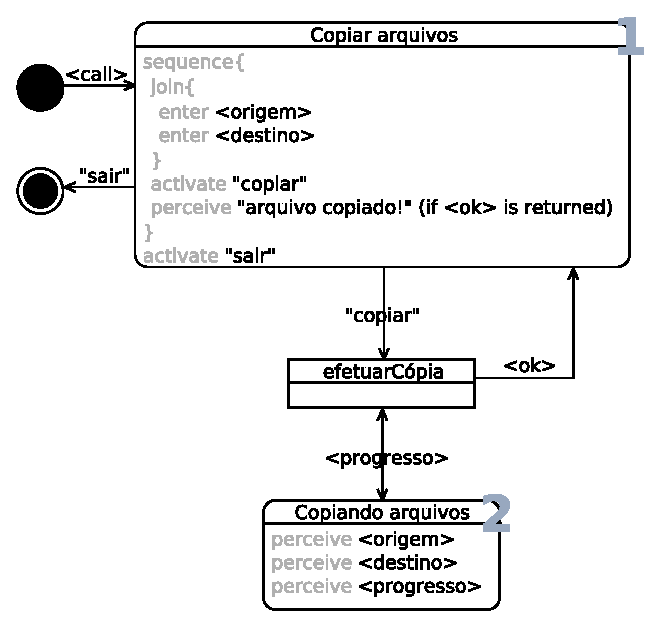
\includegraphics[scale=0.700]{images/copiarModel.eps}
    }\hspace{10mm}
    \subfigure[Lista de verificação]{
      \small
      \begin{tabular}[b]{|c|c|c|} \hline
        \multirow{2}{*}{\bf Diretriz} & 
        \multicolumn{2}{c|}{\bf Espaço de Interação} \\ \cline{2-3}

        & ~~~~~{\bf 1}~~~~~ & ~~~~~{\bf 2}~~~~~ \\ \hline

        $D_{1}$ & \na & \cf \\ \hline
        $D_{2}$ & \na & \cf \\ \hline
        $D_{3}$ & \na & \na \\ \hline
        $D_{4}$ & \cf & \na \\ \hline
        $D_{5}$ & \na & \vi \\ \hline
        $D_{6}$ & \na & \na \\ \hline
        $D_{7}$ & \na & \na \\ \hline
        $D_{8}$ & \na & \na \\ \hline
        $D_{9}$ & \cf & \cf \\ \hline
        $D_{10}$ & \cf & \cf \\ \hline
        $D_{11}$ & \na & \na \\ \hline
        $D_{12}$ & \na & \na \\ \hline
        $D_{13}$ & \cf & \na \\ \hline
        $D_{14}$ & \vi & \na \\ \hline
      \end{tabular}
    }
    \caption{Exemplo de coleta de dados feita por um avaliador durante
      a coleta de dados.}
    \label{fig:InspectionExemple}
  \end{center}
\end{figure}

A partir da  análise da figura~\ref{fig:InspectionExemple}, é possível
fazer  algumas  considerações,   sobre  dois  possíveis  problemas  de
usabilidade que poderão ser  concretizados na interface, caso ela seja
implementada com base nesse modelo de interação.  O primeiro refere-se
um  potencial  problema  relacionado  {\em  à  falta  de  prevenção  e
  recuperação  de  erros}  (categoria  $C_4$),  isso  que  porque,  se
acontecer  alguma falha  na execução  do processo  de cópia,  não está
designado  um local  onde o  usuário possa  receber  alguma informação
sobre o  problema, o que é  antecipado com a violação  de $D_{14}$, no
primeiro espaço de  interação, pois a função da  aplicação associada a
ele,  pode falhar  e não  há reações  de falha  para nenhum  espaço de
interação.

O segundo potencial problema está relacionado {\em à falta de controle
  explícito do usuário} (categoria  $C_2$), isso porque, se o usuário,
mesmo  acompanhando o  progresso  da execução  do  processo de  cópia,
julgar que  vai demorar mais do  que ele está disposto  a esperar, ele
não poderá cancelar o processo e terá obrigatoriamente que esperar até
sua conclusão, o que é antecipado  com a violação de $D_5$, no segundo
espaço de interação.

%=====================================================================
\subsection{Fases do método inspeção}
\label{inspectionMethod}
%=====================================================================

Como  se  conhece  na  literatura,  métodos  de  inspeção,  como  {\em
  avaliação     heurística}~\cite{Nielsen:1994},     {\em     percurso
  cognitivo}~\cite{Wharton:etal:1994}       e       {\em      inspeção
  semiótica}~\cite{deSouza:etal:2006} são constituídos por um conjunto
de passos ou  fases que visam instruir o  avaliador durante o processo
de  execução do  método  para  obter os  resultados  esperados em  sua
aplicação. De modo  semelhante, o método de inspeção  proposto para os
modelos \aladim, é constituído de três fases, descritas a seguir:

\begin{enumerate}

  \item  {\em  Preparação}:  Nesta  fase, os  avaliadores  preparam  o
    material usado na avaliação,  que, essencialmente, são: os modelos
    de  interação e as  fichas com  a lista  de verificação  para cada
    modelo   a   ser   inspecionado.   Contudo,   adicionalmente,   os
    avaliadores podem lançar mão dos documentos sobre os requisitos do
    sistema  para  auxiliá-los  no  entendimento sobre  o  domínio  da
    aplicação sendo avaliada.

  \item {\em  Coleta e  interpretação dos dados}:  Esta é uma  fase de
    execução  individual,  onde cada  avaliador  irá inspecionar  cada
    modelo   e  preencher   sua  respectiva   lista   de  verificação,
    atribuindo,  para  cada  espaço  de interação,  sua  avaliação  da
    diretriz, indicando  um dos seguintes  valores: {\em Conformidade}
    (\cf),  {\em Violação}  (\vi) e  {\em  Não se  aplica} (\na).   Na
    sequência,   cada   avaliador   cria   sua  lista   de   problemas
    identificados,   indicando   seu   local,  sua   severidade,   sua
    justificativa e alguma recomendação de solução.

  \item {\em Consolidação e relato dos resultados}: Esta última fase é
    de   execução  coletiva,   onde  todos   os   avaliadores  revisam
    conjuntamente suas listas  de problemas, julgando suas respectivas
    relevâncias,   severidades,    justificativas   e   recomendações.
    Finalmente,  produzem  um  relatório  consolidado,  descrevendo  o
    processo de  inspeção e  os resultados obtidos,  ou seja,  a lista
    definitiva dos problemas identificados.

\end{enumerate}

Alguns pontos precisam ser  esclarecidos sobre o processo de inspeção.
O  primeiro diz  respeito  ao fato  dos  textos da  descrição de  cada
diretriz serem  orientados aos espaços de interação.   O que significa
que as diretrizes devem ser verificadas ou confrontadas aos espaços de
interação.  Excepcionalmente, $D_{14}$  possui texto baseado na função
da aplicação.  Contudo, o avaliador  deve aplicar a diretriz ao espaço
de interação que aciona a função da aplicação, visto que, este seria o
último espaço de interação com o qual o usuário teria interagido antes
da   falha    ocorrer.    Isto   foi   demostrado    no   exemplo   da
figura~\ref{fig:InspectionExemple},  como pode  ser percebido,  que os
espaços de  interação fora enumerados  e distribuídos na tabela  com a
lista de verificação.

Considerando que a  lista de verificação tem duas  dimensões, uma para
os  espaços de  interação  e  outra para  as  diretrizes, o  avaliador
poderá,  estrategicamente, fixar  uma  diretriz e  percorrer todos  os
espaços  de interação,  ou fixar  um espaço  de interação  e percorrer
todas as diretrizes.  Por conveniência,  poderá se formatar a lista de
verificação  de  maneira   tabular,  estabelecendo,  por  exemplo,  as
diretrizes ao longo das linhas e  os espaços de interação ao longo das
colunas,    o    que    também     foi    feito    no    exemplo    da
figura~\ref{fig:InspectionExemple}.

O  segundo  aspecto  diz  respeito  ao  julgamento  da  severidade  do
problema.  Por  isso, optou-se por  permitir que o avaliador  faça uso
das abordagens propostas  por \citeonline{Nielsen:1993}, que podem ser
uma {\em escala  de classificação simples}, com valores  lineares ou a
{\em  combinação das  dimensões} associadas  ao problema.   No  que se
refere  a uma  simples  escala,  pode-se ter  os  seguintes valores  e
significados~\cite[p.~103]{Nielsen:1993}:

\begin{enumerate}[start=0]

  \item {\em isto não é, de todo, um problema de usabilidade};

  \item {\em  problema cosmético}: não  precisa ser corrigido  a menos
    que haja tempo sobrando no projeto;

  \item {\em  problema de pequena importância}: a  correção deste tipo
    de problema deve ter baixa prioridade;

  \item {\em  problema de  grande importância}: é  importante corrigir
    este  problema,  portanto,  à  sua  correção deve  ser  dada  alta
    prioridade;

  \item  {\em  problema  catastrófico}:  é  imperativo  corrigir  este
    problema antes que o produto sendo avaliado possa ser liberado;
\end{enumerate}

Ainda  é possível  usar a  abordagem  da combinação  das dimensões  do
problema,  sugeridas  por  \citeonline[p.~104]{Nielsen:1993},  onde  o
avaliador poderá considerar, por exemplo, as seguintes dimensões:

\begin{itemize}

  \item  {\em frequência}:  indica qual  a proporção  de  usuários que
    experimentaram o problema;

  \item {\em impacto}: indica qual  o dano causado pelo problema sobre
    as atividades realizadas pelo usuário que experimentou o problema;

  \item  {\em persistência}:  indica se  o problema  ocorre  apenas na
    primeira vez  que o usuário interage  com o sistema e  não mais se
    repete após superado,  ou continuará se repetindo persistentemente
    sempre que o usuário interagir com o sistema.

\end{itemize}

Vale   ressaltar   que   a    adoção   da   abordagem   proposta   por
\citeonline[p.~103-104]{Nielsen:1993}    para   a    identificação   e
tratamento da severidade dos  erros de usabilidade encontrados durante
a inspeção \aladim,  segue integralmente a proposta de  forma que mais
detalhes e exemplos podem ser obtidos diretamente na documentação.

%=====================================================================
\section{Experimento de validação do método}
\label{evaluation}
%=====================================================================

Com o objetivo de validar o método de inspeção \aladim, realizou-se um
estudo experimental,  que consistiu na inspeção de  um modelo \aladim,
usando  as diretrizes  definidas  na seção~\ref{inspectionGuidelines},
visando  a identificação  de problemas  de usabilidade.   O  modelo de
interação utilizado resultou da  engenharia reversa da interface usada
para realização de uma tarefa, na agência virtual de um banco estatal.

Os resultados  das inspeções foram  confrontados aos resultados  de um
teste de usabilidade executado  na referida interface, que serviram de
gabarito,   confirmando  se   determinado   problema  de   usabilidade
identificado durante a inspeção  do modelo foi, de fato, experimentado
pelo usuário, durante o teste de usabilidade.  A seguir, é apresentado
o {\em gabarito} e como seu  deu sua construção, bem como a definição,
o planejamento, a execução, a  operação, validação dos dados e análise
\&   interpretação   do    experimento,   nos   moldes   da   proposta
\citeonline{Wohlin:etal:2000},    para    engenharia    de    software
experimental.

%=====================================================================
\subsection{Construção do gabarito}
\label{initialExperiments}
%=====================================================================

Como será definido na seção~\ref{studyGoal}, o experimento comparou os
resultados   da   inspeção   em   modelos   \aladim,   com   problemas
comprovadamente  já experimentados  pelos usuários,  durante o  uso do
sistema  objeto  de  inspeção  no experimento.   Esse  {\em  gabarito}
resulta dos dados de um teste de usabilidade previamente executado por
\citeonline{CostaNeto:etal:2011},  cuja  descrição  e  resultados  são
resumidos a seguir.

O   teste   envolveu   cinco   participantes,  todos   estudantes   de
pós-graduação e com  uma média de três anos de  experiência no uso dos
serviços do banco.   Cada sessão de teste foi  composta de duas fases.
A  primeira consistiu  das orientações  de como  seriam  realizados os
testes.  A segunda consistiu da atuação do usuário no uso do sistema e
respondendo  às  perguntas  realizadas  pelos  avaliadores  durante  a
interação.

Considerando que, atualmente, a maioria dos bancos oferece serviços de
{\it internet bank} aos seus  clientes e que não é incomum reclamações
de usuários que encontram algum tipo de dificuldade em utilizar alguns
desses serviços.   No referido trabalho,  o teste avaliou a  tarefa de
{\em adesão ao serviço de envio de mensagens SMS}, oferecido pela {\it
  Caixa Econômica Federal}, cujo cenário é descrito a seguir.

\begin{citacao}

  O cenário começa quando um cliente, na página principal, seleciona a
  opção  {\em  Mensagem  via  celular  - SMS},  então  o  sistema  lhe
  apresenta uma  breve explicação sobre  o serviço e  disponibiliza ao
  cliente  duas opções:  {\em  Excluir} e  {\em  Incluir}.  O  cliente
  seleciona  a  opção  {\em  Incluir},  depois disso,  o  sistema  lhe
  apresenta informações mais detalhadas sobre o serviço e mais algumas
  opções, dentre  elas a opção de {\em  Continuar}.  Selecionando {\em
    Continuar}, é  apresentado ao cliente  o {\em Termo de  Adesão} no
  qual ele tem a opção de {\em Concordar}.  Após marcar essa intenção,
  o  sistema solicita  os dados  sobre o  número do  telefone  que irá
  receber as mensagens  e a faixa de valores  das transações e oferece
  ao cliente  a opção  {\em Cadastrar}.  Após  o usuário  pressionar o
  botão {\em  Cadastrar}, o sistema  apresenta as informações  sobre a
  adesão e  solicita a  senha da  conta, o cliente  informa a  senha e
  seleciona {\em Confirmar}, o sistema  então informa ao cliente que a
  conta já está cadastrada~\cite[p.~128]{CostaNeto:etal:2011}.

\end{citacao}

Como  forma  de identificar  se  o  diálogo  apresentado pelo  sistema
avaliado possibilitava uma sequência  clara de interações, sob o ponto
de  vista do  usuário,  foram elaboradas  algumas  questões que  foram
aplicadas durante  a interação.  Estas  questões tinham o  objetivo de
conhecer o pensamento  do usuário e eram solicitadas  a cada página da
interface  apresentada durante  a observação  do sistema  em  uso. São
elas:

\begin{enumerate}
  \renewcommand{\labelenumi}{\alph{enumi})}

  \item Você consegue identificar onde está? Porque?
  \item O que você acha que pode/deve fazer agora? Porque?
  \item O que você acha que o sistema vai fazer a partir dessas ações?
    Porque?
\end{enumerate} 

É importante  ressaltar que nas intervenções  feitas pelos avaliadores
foram realizadas de  forma a não interferir na  experiência de uso dos
participantes,  ou seja,  limitou-se  apenas a  ouvir  e registrar  as
respostas  dadas  para  cada   questão.   Desta  forma,  foi  possível
identificar quais fatores ou problemas de usabilidade não permitiam ao
usuário saber, através  da interação, qual o estado  atual do sistema,
as possíveis ações que ele  podia executar e quais seriam os possíveis
efeitos destas ações.   Cada sessão de teste foi  registrada em áudio,
vídeo e  formulários, que foram  usados para coletar as  respostas dos
usuários às questões acima.  Estes registros foram produzidos usando a
ferramenta      {\em      RecordMyDesktop}\footnote{Disponível      em
  http://recordmydesktop.sourceforge.net}.

A  partir  da  lista  de  problemas encontrados  durante  o  teste  de
usabilidade, associou-se  cada problema  encontrado a uma  diretriz do
método de  inspeção, indicando que  o problema teria sido  causado por
sua  violação,  o  que  resultou  na  tabela~\ref{tab:testeProblemas}.
Também  foram indicadas as  diretrizes que  estavam em  conformidade e
quais não  se aplicavam aos  problemas encontrados.  Esse  processo de
associação,  produziu  a  lista   de  verificação  que  foi  usada  na
comparação   com  os   resultados  das   inspeções   realizadas  pelos
participantes         do         experimento,         feita         na
tabela~\ref{tab:DiretrizesFrequencia}, da  apresentação da estatística
descrita do experimento (seção~\ref{descriptiveStatistics}).

% Tabela dos problemas encontrados durante os testes de usabilidade
\begin{table}[!htb]
  \small
  \begin{center}
    \begin{tabular}{|c|m{76mm}|m{48mm}|c|} \hline

      {\bf \#} & {\bf Descrição} & {\bf Local/Página} & {\bf Violação}
      \\ \hline

      1 & O usuário não sabia em que ponto da tarefa estava.  & {\em 1
        - Selecionar conta} & $D_{3}$ \\ \hline

      2 & O usuário se questiona se incluir é a mesma coisa que aderir
      ao serviço.  & {\em 1 - Selecionar conta} & $D_{10}$ \\ \hline

      3 & O usuário se questiona  se já tivesse aderido e possuísse um
      telefone registrado.   & {\em 1  - Selecionar conta}  & $D_{13}$
      \\ \hline

      4 & O usuário não sabia em  que ponto da tarefa estava. & {\em 2
        - Apresentação do serviço} & $D_{3}$ \\ \hline

      5 & O usuário não sabia em que ponto da tarefa estava.  & {\em 3
        - Termo de adesão} & $D_{3}$ \\ \hline

      6 & O  usuário pretende voltar à página  anterior, mas o sistema
      não permitiu.  & {\em 3 - Termo de adesão} & $D_{7}$ \\ \hline

      7 & O  participante é levado à página  de {\em Selecionar conta}
      (início do cenário) ao clicar  no botão {\em Discordo}. & {\em 3
        - Termo de adesão} & $D_{11}$ \\ \hline

      8 & O participante se confunde sobre que ponto da tarefa está de
      fato. & {\em 4 - Dados para adesão} & $D_{3}$ \\ \hline

      9 & O  usuário pretende voltar à página  anterior, mas o sistema
      não permitiu.  & {\em 4 - Dados para adesão} & $D_{7}$ \\ \hline

      10 & O participante é  levado à página de {\em Selecionar conta}
      (inicio do cenário) ao clicar no botão {\em Retornar}.  & {\em 4
        - Dados para adesão} & $D_{11}$ \\ \hline

      11 & O  participante se confunde sobre que  ponto da tarefa está
      de fato.  & {\em 5 - Confirmação dos dados} & $D_{3}$ \\ \hline

      12 & O usuário pretende  voltar à página anterior, mas o sistema
      não  permitiu. &  {\em  5  - Confirmação  dos  dados} &  $D_{7}$
      \\ \hline

      13 & O participante é  levado à página de {\em Selecionar conta}
      (inicio do cenário) ao clicar no botão {\em Cancelar}.  & {\em 5
        - Confirmação dos dados} & $D_{11}$ \\ \hline

      14 & O usuário pretende  voltar à página anterior, mas o sistema
      não  permitiu.   & {\em  5  -  Conta  já cadastrada}  &  $D_{7}$
      \\ \hline

      15 & O participante é  levado à página de {\em Selecionar conta}
      (inicio do cenário) ao clicar no botão {\em Voltar}.  & {\em 5 -
        Conta já cadastrada} & $D_{11}$ \\ \hline

    \end{tabular}
    \caption{Problemas encontrados durante o teste de usabilidade.}
    \label{tab:testeProblemas}
  \end{center}
\end{table}

%=====================================================================
\subsection{Definição do experimento}
\label{experimentDefining}
%=====================================================================

De acordo com \citeonline{Wohlin:etal:2000}, é nesta fase que ocorre a
concepção  do experimento, através  da definição  de quais  os objetos
serão estudados, quais os  propósitos do estudo, quais características
dos objetos serão estudas,  sob quais perspectivas os resultados serão
interpretados e em  qual ambiente o estudo irá  ocorrer.  Dessa forma,
considerando         o          guia         prático,         proposto
por~\citeonline{Solingen:Berghout:1999}   para  aplicação   do  método
\gqm\ ({\em \Gqm}) de~\citeonline{Basili:etal:1994}, são apresentados,
a seguir, o objetivo, as questões e as métricas deste experimento.

%=====================================================================
\subsubsection{Objetivo}
\label{studyGoal}
%=====================================================================

Considerando          o          esquema         proposto          por
\citeonline[p.~51]{Solingen:Berghout:1999}, este  estudo visa analisar
           {\em  o  método de  inspeção  de  modelos  \aladim}, com  o
           propósito  de  {\em   caracterizar}  a  sua  capacidade  de
           identificação antecipada  de problemas de  usabilidade, com
           respeito à  sua {\em  eficácia}, em comparação  à avaliação
           feita sobre  o sistema em uso,  do ponto de  vista dos {\em
             avaliadores   de  usabilidade},   no  contexto   do  {\em
             desenvolvimento de sistemas interativos}.

%=====================================================================
\subsubsection{Questões}
\label{studyQuestions}
%=====================================================================

Visando alcançar o objetivo estabelecido acima e considerando o método
proposto  por  \citeonline{Solingen:Berghout:1999},  este  experimento
busca responder as seguintes questões:

\begin{enumerate}
  \renewcommand{\labelenumi}{$Q_{\arabic{enumi}}$}

  \item A  inspeção permitiu identificar os  problemas apresentados no
    gabarito, isto é, que foram encontrados em ambas as avaliações?

  \item A inspeção identificou  problemas que não estavam no gabarito,
    isto é, não foram encontrados apenas na inspeção?

  \item A inspeção não identificou problemas apresentados no gabarito,
    isto é, que foram encontrados apenas no teste de usabilidade?

  \item  O  método  de  inspeção,  usando  o  conjunto  de  diretrizes
    apresentado, foi considerado aceitável pelos participantes?

\end{enumerate}

%=====================================================================
\subsubsection{Métricas}
\label{studyMetrics}
%=====================================================================

Para responder às questões da seção~\ref{studyQuestions}, é necessário
estabelecer algumas  métricas. Para as três primeiras  questões, o que
se  pretende medir,  são  os problemas  identificados  na inspeção  em
comparação  com  os problemas  encontrados  no  teste de  usabilidade.
Contudo,  cada  problema  encontrado   no  teste  de  usabilidade  foi
associado a  uma das diretrizes  do método de inspeção,  produzindo um
gabarito  com uma  lista de  verificação das  diretrizes  violadas, em
conformidade  e  não  aplicadas, vide  seção~\ref{initialExperiments}.

Dessa forma,  o que se precisa  medir são os números  de diretrizes em
conformidade, violadas  e não aplicadas  do gabarito em  comparação às
listas  de  verificação  preenchidas  pelos participantes  durante  as
sessões de inspeção. Por isso, optou-se por fazer uso de uma matriz de
confusão~\cite{Tan:etal:2005}, apresentada na tabela~\ref{tab:matriz},
onde  as linhas  representam a  {\em classe  real}  (classificação das
diretrizes feita durante as inspeções) e as colunas representam a {\em
  classe predita} (classificação das diretrizes no gabarito).  Onde os
valores representam, respectivamente: {\bf 1} -- Conformidade, {\bf 2}
-- Violação,  {\bf 3}  --  Não se  aplica.   Portanto, empregou-se  as
seguintes métricas para as respectivas questões:

\begin{enumerate}

  \renewcommand{\labelenumi}{$Q_{\arabic{enumi}}$}

  \item Esta questão foi medida pelo número de problemas identificados
    na inspeção e  que constavam no gabarito do  teste de usabilidade,
    isto é,  onde as diretrizes  foram violadas nas duas  situações, o
    que corresponde aos elementos $f_{22}$ da matriz de confusão.

  \item Esta questão foi medida pelo número de problemas identificados
    na inspeção mas não constavam no gabarito do teste de usabilidade,
    isto  é, onde  as diretrizes  estavam  em conformidade  ou não  se
    aplicavam no teste de usabilidade, o que corresponde aos elementos
    $f_{21}$ e $f_{23}$ da matriz de confusão.

  \item Esta questão foi medida pelo número de problemas que constavam
    no gabarito do teste, mas que não foram identificados na inspeção,
    isto  é onde  as  diretrizes  estavam em  conformidade  ou não  se
    aplicavam na inspeção, o  que corresponde aos elementos $f_{12}$ e
    $f_{32}$ da matriz de confusão.

  \item Esta questão foi medida  pela análise dos dados produzidos por
    uma      adaptação      do      formulário      SUS,      proposto
    por~\citeonline{Brooke:1996}.

\end{enumerate}

\begin{table}[!htb]
 \begin{center}
   \begin{tabular}{|c|c|c|c|c|} \cline{3-5}
     \multicolumn{2}{c|}{} &
     \multicolumn{3}{c|}{\bf Gabarito} \\ \cline {3-5}

     \multicolumn{2}{c|}{} & 
     {\bf \cf~~(1)} & {\bf \vi~~(2)} & {\bf \na~~(3)}  \\ \hline

     \multirow{3}{*}{\bf Inspeção} & {\bf \cf~~(1)} & 

%     \cellcolor{blue!25}
     $f_{11}$ & $f_{12}$ & $f_{13}$ \\ \cline{2-5}

     & {\bf \vi~~(2)} & 
     $f_{21}$ & $f_{22}$ & $f_{23}$ \\ \cline{2-5}

     & {\bf \na~~(3)} & 
     $f_{31}$ & $f_{32}$ & $f_{33}$ \\ \hline

   \end{tabular}
   \caption{Matriz           de           confusão,           adaptada
     de~\citeonline[p.~169]{Tan:etal:2005}.}
   \label{tab:matriz}
 \end{center}
\end{table}

%=====================================================================
\subsection{Planejamento}
\label{planning}
%=====================================================================

Segundo  \citeonline{Wohlin:etal:2000}, esta fase  é composta  de sete
atividades,  a seleção  do  contexto, a  formulação  das hipóteses,  a
seleção  de  variáveis,  a  seleção  dos participantes,  o  modelo  do
experimento,  a instrumentação  e  a avaliação  de  validade, que  são
apresentadas a seguir.

%=====================================================================
\subsubsection{Seleção do contexto}
\label{contextSelection}
%=====================================================================

Esta  atividade visa caracterizar  o contexto  onde o  experimento foi
realizado. Segundo  \citeonline{Wohlin:etal:2000}, esta caracterização
deve cobrir as seguintes dimensões:

\begin{itemize}

  \item {\em Processo}: o experimento não foi executado em um processo
    formal de  desenvolvimento de software, ou seja,  foi executado em
    um processo {\em off-line};

  \item {\em  Participantes}: o experimento não foi  executado por uma
    equipe de profissionais, mas por uma equipe de {\em estudantes} da
    área de computação;

  \item  {\em  Realidade}:  o  experimento  endereçou  problemas  {\em
    reais}, encontrados na agência virtual de um banco;

  \item {\em  Generalidade}: o  experimento não pode  ser generalizado
    por  ser válido  apenas  para o  contexto  {\em específico}  deste
    estudo.

\end{itemize}

%=====================================================================
\subsubsection{Definição das hipóteses}
\label{hypothesisFormulation}
%=====================================================================

O principal fundamento para análise  estatística de um experimento é o
teste  de  hipótese.  Para  isso,  uma  ou  mais hipóteses  devem  ser
formuladas, deixando  claro o que se pretende  avaliar no experimento.
Buscando avaliar  o grau de  concordância entre as  classificações das
diretrizes,  no  gabarito  e  nas  inspeções,  foi  empregado  o  {\em
  Coeficiente Kappa},  proposto por~\citeonline{Cohen:1960} e definido
pela  equação~\ref{eq:Kappa}.  Sendo  que este  experimento  partiu da
hipótese que  há concordância entre a classificação  das diretrizes no
gabarito e  nas inspeções.  Dessa forma, as  seguintes hipóteses foram
consideradas:

\begin{itemize}

  \item {\em Nula}: não há concordância entre a classificação feita no
    teste e a classificação feita na inspeção, ou seja $H_0$: $k = 0$.

  \item   {\em   Alternativa}:   há   alguma  concordância   entre   a
    classificação feita no teste  e a classificação feita na inspeção,
    ou seja, $H_1$: $k > 0$

\end{itemize}

\begin{equation}
  k = \frac{p_{o} - p_{e}}{1 - p_{e}}
  \label{eq:Kappa}
\end{equation}

\begin{tabular}{cl}
  sendo: & 
  $p_{o} = \frac{acertos}
  {acertos + erros}$ \\
  & $p_{e} = \displaystyle\sum_{i=1}^{n}(p_{i1} \times p_{i2})$
\end{tabular}

\begin{tabular}{ll}
  onde: 

  & $acertos=$ soma  dos elementos da diagonal principal  da matriz de
  confusão\\

  & $erros=$ soma  dos elementos fora da diagonal  principal da matriz
  de confusão\\

  & $n =$ número de categorias\\
  & $i =$ número da categoria (de $1$ até $n$)\\

  &  $p_{i1} =$  proporção  de  ocorrência da  categoria  $i$ no  {\em
    gabarito}\\

  &  $p_{i2} =$  proporção  de  ocorrência da  categoria  $i$ na  {\em
    inspeção}

\end{tabular}

%=====================================================================
\subsubsection{Seleção de variáveis}
\label{variablesSelection}
%=====================================================================

Nesta   fase,   foram   selecionadas   as  variáveis   dependentes   e
independentes,  que  representam,  respectivamente  as entradas  e  os
resultados  do  processo  de  experimentação.  Neste  experimento,  as
variáveis definidas foram as seguintes:

\begin{itemize}

  \item {\em Independentes} (entradas): o modelo de interação descrito
    em \aladim\ e a lista de verificação usados na inspeção e gabarito
    resultante do teste usado na comparação;

  \item {\em Dependentes} (resultados):  as listas de verificações com
    as  classificações  das  diretrizes  nas  inspeções e  o  grau  de
    concordância entre inspeção e gabarito na comparação;

\end{itemize}

%=====================================================================
\subsubsection{Seleção dos participantes}
\label{subjectsSelection}
%=====================================================================

A  abordagem   escolhida  para  a  seleção   dos  participantes  deste
experimento  é feita  por  conveniência, ou  seja, foram  selecionados
dezenove alunos  da disciplina {\em Projeto de  Interface de Usuário},
dos  cursos  de graduação  em  {\em  Engenharia  de Software}  e  {\em
  Ciências da Computação}, da  {\em Universidade Federal do Rio Grande
  do Norte}.

%=====================================================================
\subsubsection{Modelo do experimento}
\label{experimentDesign}
%=====================================================================

Apesar deste  experimento procurar comparar o  resultado das inspeções
com o resultado previamente  estabelecido, seu modelo experimental foi
considerado      do      tipo       ``um      fator      com      dois
tratamentos''~\cite[p.~54]{Wohlin:etal:2000}, que foram definidos como
entradas  ou variáveis  independentes. Mesmo  o resultado  do primeiro
tratamento  (considerado aqui,  o teste  de usabilidade)  já  ter sido
produzido, buscou-se garantir os seguintes princípios:

\begin{itemize}

  \item {\em Aleatorização}: Neste experimento, todos os participantes
    aplicaram o  mesmo tratamento (inspeção)  sobre o mesmo  objeto ao
    mesmo tempo,  dessa maneira, não foi  preciso aleatorizar qualquer
    ordem na execução dos testes.

  \item  {\em  Bloqueio}: Neste  experimento  não foram  identificados
    fatores  que  pudessem   causar  efeitos  indesejáveis,  dadas  as
    condições de execução dos testes. Contudo, diante da possibilidade
    de  não saber o  quanto os  participantes aprenderam  \aladim, bem
    como o  entendimento das diretrizes,  considerou-se eliminar dados
    que  estivessem longe  da  média  geral da  turma,  como visto  na
    seção~\ref{operationValidation}.

  \item   {\em  Balanceamento}:   Neste  experimento,   não   houve  a
    necessidade  de   se  realizar  o  balanceamento,   visto  que  os
    participantes   tinham  o  mesmo   perfil,  receberem   as  mesmas
    informações  sobre  o  método  de  inspeção e  aplicaram  o  mesmo
    tratamento ao mesmo objeto e ao mesmo tempo.

\end{itemize}

%=====================================================================
\subsubsection{Instrumentação}
\label{experimentInstrumentation}
%=====================================================================

Consiste  da descrição  dos instrumentos  que foram  usados  durante a
execução      dos       testes      do      experimento.       Segundo
\citeonline{Wohlin:etal:2000}, os  instrumentos são de  três tipos: os
objetos, as  guias e as medições.   Neste experimento, o  objeto foi o
modelo de  interação, usando a  linguagem \aladim, produzido  a partir
das  interfaces do  sistema avaliado,  para a  mesma  tarefa realizada
durante o teste de usabilidade (seção~\ref{initialExperiments}), que é
apresentado na figura~\ref{fig:CookieModel}.

\figura{Modelo de interação inspecionada durante o experimento.}
       {fig:CookieModel}
       {cookieModel.eps}
       {0.700}
       {-90}

Para  guiar  os  participantes  no experimento,  os  mesmos  receberam
treinamento na linguagem \aladim, bem como esclarecimentos sobre o uso
das  diretrizes,  visto  que  cada teste  experimental  (aplicação  do
tratamento  ao  objeto   pelo  participante)  consistiu  da  atividade
inspeção do modelo \aladim.   Além disso, para realização da inspeção,
os  participantes  seguiram  a  {\em  lista  de  verificação}  com  as
diretrizes.

As  medições  foram realizadas  por  meio  da  coleta de  informações,
durante  as  sessões  de  teste  experimental,  inspeção.   Assim,  os
problemas de usabilidade identificados foram medidos por meio das {\em
  listas de  verificações}, já o  perfil dos participantes  foi medido
por meio do questionário pré-teste, enquanto que a aceitação do método
foi medida  por meio de  questionário pós-teste, que consistiu  de uma
adaptação do formulário SUS proposto por \citeonline{Brooke:1996}.

%% Todos  os  instrumentos usados  no  experimento,  são apresentados  no
%% apêndice~\ref{} deste documento.

%=====================================================================
\subsubsection{Avaliação da validade}
\label{validityEvaluation}
%=====================================================================

Consiste em  assegurar que  os resultados produzidos  pelo experimento
sejam válidos, no mínimo para a amostra da população que foi submetida
aos testes. Como os resultados  dos testes de usabilidade foram usados
como gabarito, assume-se a validade mínima do mesmo, sobre sua amostra
de participantes.  Assim, considerando os tipos de validades definidos
por \citeonline{Wohlin:etal:2000}, neste experimento, eles foram assim
avaliados:

\begin{itemize}

  \item {\em  Conclusão}: Com a  finalidade de se  realizar conclusões
    válidas sobre  o experimento, foi usado o  {\em Coeficiente Kappa}
    (seção~\ref{hypothesisFormulation})   para   medir   o   grau   de
    concordância entre  as classificações  das diretrizes em  ambas as
    avaliações.   Para uma  boa  compreensão do  grau de  concordância
    foram        usadas       as        interpretações       sugeridas
    por~\citeonline{Landis:Koch:1977}.

  \item  {\em Interna}:  Os participantes  executaram  suas inspeções,
    individualmente, para que nenhum tivesse influência de outro.

  \item {\em Construção}:  Por se tratar de um  método de avaliação de
    usabilidade, foi usada a  quantidade de problemas encontrados, por
    ser  um importante  indicador  de produtividade  do método.   Além
    disso,  foi  usado  o  formulário  SUS que  possui  seus  próprios
    indicadores de  confiança das respostas  coletadas.  Como apontado
    no trabalho  de~\citeonline{Tullis:Stetson:2004}, ele apresentou o
    melhor  percentual   de  conclusões  corretas,   sobre  os  demais
    estudados, em amostras superiores a oito indivíduos.

  \item  {\em Externa}:  Apesar  de não  se  pretender generalizar  as
    conclusões deste experimento,  todos os participantes selecionados
    possuíam  o perfil  adequado, assim  como  o ambiente  e o  tempo,
    necessários para sua execução, também foram adequados.

\end{itemize}

%=====================================================================
\subsection{Operação}
\label{operation}
%=====================================================================

Após  definido   e  planejado,  o   experimento  foi  operacionalmente
conduzido  de maneira que  se pode  coletar os  dados, posteriormente,
analisados.    Segundo  \citeonline{Wohlin:etal:2000},  esta   fase  é
constituída dos passos de preparação, execução e validação dos dados.

%=====================================================================
\subsubsection{Preparação}
\label{operationPrepartation}
%=====================================================================

A todos  os participantes foram dados esclarecimentos,  sobre todos os
aspectos  étnicos  envolvidos  na  participação  de  cada  um.   Foram
garantidos, o anonimato e  a possibilidade de desistir da participação
a  qualquer momento.   Os questionários  pré e  pós-teste, bem  como a
lista   de  verificação   necessários   à  coleta   dos  dados   foram
disponibilizados.

%=====================================================================
\subsubsection{Execução}
\label{operationExecution}
%=====================================================================

Imediatamente antes da  seção de testes, o moderador  expôs o que cada
participante deveria executar,  explicando as diretrizes e demostrando
um exemplo  de como preencher a  lista de verificação, a  partir de um
modelo  usado  para  esta   finalidade.   Durante  toda  a  sessão  de
inspeções,  o moderador  ficou  à disposição  para esclarecer  dúvidas
eventuais.   A coleta  de dados  foi feita  pelo  próprio participante
através  do  preenchimento dos  questionários  pré  e  pós-teste e  do
preenchimento do {\em lista de verificação}.

%=====================================================================
\subsubsection{Validação dos dados}
\label{operationValidation}
%=====================================================================

Foram  eliminados   da  análise,   os  dados  dos   participantes  que
preencheram erroneamente quaisquer dos  materiais de coleta. Em função
da aplicação dos testes experimentais, terem ocorridos em sala de aula
com participação de todos os  alunos da turma, também foram eliminados
os dados  dos alunos que não  participaram da seção  de treinamento na
linguagem \aladim, bem como na aplicação das diretrizes.

A partir  das médias  de diretrizes em  conformidades, violadas  e não
aplicadas,  foi  observado  que   os  dados  de  alguns  participantes
encontravam-se  distante dessas  médias.  Dessa  forma,  optou-se pela
{\em  média truncada  ou podada},  calculada a  partir da  remoção dos
dados de dois participantes, um  de cada extremo, ficando para análise
os dados de dezessete participantes.

Para  o preenchimento do  questionário pós-teste,  dois participantes,
por algum motivo não identificado, não preencherem o formulário SUS, o
que  reduziu  os  dados  deste  formulário para  um  total  de  quinze
participantes.

%=====================================================================
\subsection{Análise e interpretação}
\label{analysis}
%=====================================================================

Após a  coleta e  validação dos dados  produzidos na fase  de operação
(seção~\ref{operation}),    estes   precisaram   ser    analisados   e
interpretados.  Esta  fase é  constituída pelos passos  de estatística
descritiva e teste de hipótese, apresentados a seguir.

%=====================================================================
\subsubsection{Estatística descritiva}
\label{descriptiveStatistics}
%=====================================================================

Aqui busca-se descrever e  representar graficamente vários aspectos de
interesse sobre  os dados.  Entre  os aspectos incluem-se  medidas que
indiquem, por exemplo, como alguma escala está posicionada no conjunto
de dados,  bem como o quanto  o conjunto de dados  está concentrado ou
espalhado.  Dessa  forma, pode-se  obter algumas medidas  de tendência
central e dispersão, como mediana, mínimos e máximos.

No  que se  refere ao  quantitativo de  diretrizes e  suas categorias,
apresentado   na   figura~\ref{fig:DiretrizesSumario},  foi   possível
observar as  medidas para classificação das  diretrizes nas categorias
conformidade, violação e não se aplica foram, respectivamente, mediana
de 8, 4 e 1, com máximos de 11, 8 e 5 e mínimos de 5, 1 e 0.

\figura{Sumário da classificação das diretrizes.}
       {fig:DiretrizesSumario}
       {diretrizesSumario.eps}
       {0.850}
       {0}

No  que se  refere  à distribuição  da  classificação das  diretrizes,
representada  na  figura~\ref{fig:DiretrizesFrequencia}, foi  possível
observar que  algumas diretrizes foram  classificadas numa determinada
categoria  por mais de  $^2/_3$ dos  participantes, como  é o  caso da
categoria  de  {\em  Conformidade}.   Enquanto outras,  não  foram  em
determinada categoria por  nenhum dos participantes, como é  o caso da
categoria {\em Não se aplica}.

\figura{Frequência de distribuição de avaliação das diretrizes.}
       {fig:DiretrizesFrequencia}
       {diretrizesFrequencia.eps}
       {0.750}
       {0}

Vale ressaltar  que a classificação  de cada diretriz  foi determinada
pela       categoria        de       maior       frequência.        Na
tabela~\ref{tab:DiretrizesFrequencia}, são  apresentados os resultados
de classificação feita no gabarito  e nas inspeções do modelo \aladim,
sendo  que esta  foi determinada  pela maior  frequência  relativa, ou
seja, a  classificação que foi definida pela  maioria dos avaliadores,
acompanhada da  respectiva frequência.  Para  caso de empate  entre as
maiores  frequências,  o desempate  seguiu  uma  ordem de  prioridade,
estabelecida entre  as categorias, que  foi {\em violação}  sobre {\em
  conformidade} e {\em conformidade} sobre {\em não se aplica}.

Com  as listas  de verificação  com as  classificações  resultantes do
teste    de   usabilidade   e    das   inspeções,    apresentadas   na
tabela~\ref{tab:DiretrizesFrequencia},  procedeu-se  a  construção  da
matriz de confusão (tabela~\ref{tab:matrizResultado}), onde nas linhas
estão  as  classificações  obtidas  nas  inspeções e  nas  colunas  as
classificações preditas (gabarito) que  foram obtidas durante o teste.
A partir  dos números  obtidos na matriz  de confusão e  dos problemas
associados  às diretrizes  violadas (tabela~\ref{tab:testeProblemas}),
foram  estabelecidas as  métricas  (seção~\ref{studyMetrics}), com  as
quais foi possível  responder às questões (seção~\ref{studyQuestions})
do experimento, conforme descrições a seguir.

\begin{table}[!htb]
  \begin{center}

     \begin{tabular}{|c|c|c|c|} \hline
      {\bf Diretriz} & {\bf Gabarito} &{\bf Inspeção} & {\bf Frequência} \\ \hline

      $D_{1}$  & \na & \na & 47,06\% \\ \hline % 3
      $D_{2}$  & \cf & \cf & 76,47\% \\ \hline % 1
      $D_{3}$  & \vi & \cf & 47,06\% \\ \hline % 1
      $D_{4}$  & \cf & \cf & 52,94\% \\ \hline % 1
      $D_{5}$  & \na & \na & 41,18\% \\ \hline % 3
      $D_{6}$  & \na & \cf & 88,24\% \\ \hline % 1
      $D_{7}$  & \vi & \vi & 47,06\% \\ \hline % 2
      $D_{8}$  & \na & \vi & 47,06\% \\ \hline % 2
      $D_{9}$  & \cf & \cf & 82,35\% \\ \hline % 1
      $D_{10}$ & \vi & \cf & 82,35\% \\ \hline % 1
      $D_{11}$ & \vi & \vi & 47,06\% \\ \hline % 2
      $D_{12}$ & \cf & \cf & 94,12\% \\ \hline % 1
      $D_{13}$ & \vi & \vi & 47,06\% \\ \hline % 2
      $D_{14}$ & \cf & \cf & 76,47\% \\ \hline % 1
    \end{tabular}
    \caption{Classificação das diretrizes no teste e na inspeção.}
    \label{tab:DiretrizesFrequencia}
  \end{center}
\end{table}

Métrica  associada  à questão  $Q_1$,  que  é  o número  de  problemas
identificados  em ambas  avaliações.  Considerando  que as  {\em três}
diretrizes  classificadas como  violadas tanto  no gabarito  quanto na
inspeção  (elementos $f_{22}$  da matriz  de confusão)  foram $D_{7}$,
$D_{11}$  e  $D_{13}$ e  que  elas  estavam  associadas a  {\em  nove}
problemas de  usabilidade, é  possível afirmar que  {\bf sim},  a {\em
  inspeção  sobre  modelos  identificou  problemas  que  foram  também
  encontrados no teste de usabilidade}.

Métrica  associada  à questão  $Q_2$,  que  é  o número  de  problemas
identificados  durante a inspeção,  mas que  não foram  encontrados no
teste.    Considerando   que  a   diretriz   classificada  como   {\em
  conformidade}  ou   {\em  não  se   aplica}  no  gabarito   mas  foi
classificada como  {\em violada}  pela inspeção (elementos  $f_{21}$ e
$f_{23}$  da matriz  de confusão)  foi $D_{8}$  e que  ela  não estava
associada a nenhum dos problemas  presentes no teste de usabilidade, é
possível  afirmar   que  {\bf  sim},  a   {\em  inspeção  identificou,
  erroneamente, problemas que  não foram experimentados pelos usuários
  durante o teste}.

\begin{table}[!htb]
 \begin{center}

   \begin{tabular}{|c|c|c|c|c|} \cline{3-5}
     \multicolumn{2}{c|}{} &
     \multicolumn{3}{c|}{\bf Gabarito} \\ \cline {3-5}

     \multicolumn{2}{c|}{} & 
     {\bf \cf~~(1)} & {\bf \vi~~(2)} & {\bf \na~~(3)}  \\ \hline

     \multirow{3}{*}{\bf Inspeção} & {\bf \cf~~~(1)} & 

     5 & 2 & 1 \\ \cline{2-5}

     & {\bf \vi~~(2)} & 
     0 & 3 & 1 \\ \cline{2-5}

     & {\bf \na~~~(3)} & 
     0 & 0 & 2 \\ \hline

   \end{tabular}
   \caption{Matriz de confusão para avaliação final do experimento.}
   \label{tab:matrizResultado}
 \end{center}
\end{table}

Métrica associada  à questão  $Q_3$, que é  o número de  problemas que
foram  encontrados  no  teste,  mas  que não  foram  identificados  na
inspeção. Considerando que as {\em duas} diretrizes classificadas como
violadas no gabarito, mas que foram classificadas como conformidade ou
não se aplica na inspeção  (elementos $f_{12}$ e $f_{32}$ da matriz de
confusão) foram  $D_{3}$ e  $D_{10}$ e que  elas estavam  associadas a
{\em seis} problemas de usabilidade, é possível afirmar que {\bf sim},
a  {\em  inspeção  de  modelos  não identificou  problemas  que  foram
  encontrados durante o teste}.

Para  responder a  questão  $Q_4$, verificou-se  o  grau de  aceitação
medido pelo formulário SUS.  \citeonline[p.192]{Brooke:1996} apresenta
o  procedimento  para  se  calcular  o  grau  de  aceitação  usando  o
questionário.    Os  valores  obtidos   para  cada   participante  são
apresentados na figura~\ref{fig:SusResultados}.   Onde, os dados foram
sumarizados com  o mínimo de  45, máximo de  82,5 e mediana  de 68,75.
Considerando que  o grau de aceitação  médio da turma foi  de 66,88 e,
também,              considerando              o              trabalho
de~\citeonline[p.~118]{Bangor:etal:2009}, pode-se  concluir que o grau
de aceitação  médio foi considerado satisfatório por  ficar entre {\em
  OK} (50,9) e {\em Good} (71,4).

\begin{figure}[!htb]
  \begin{center}

    \subfigure[Valores do grau de aceitação]{
      \small
      \begin{tabular}[b]{|c|c|c|c|} \hline
        {\bf \#} & {\bf Idade} & 
        {\bf Sexo} & {\bf Grau} (SUS) \\ \hline

        $p_{1}$ & 24 & Masculino & 77,50 \\ \hline
        $p_{2}$ & 19 & Feminino & 72,50 \\ \hline
        $p_{3}$ & 21 & Masculino & 82,50 \\ \hline
        $p_{4}$ & 19 & Masculino & 57,50 \\ \hline
        $p_{5}$ & 20 & Masculino & 67,50 \\ \hline
        $p_{6}$ & 23 & Masculino & 77,50 \\ \hline
        $p_{7}$ & 21 & Feminino & 75,00 \\ \hline
        $p_{8}$ & 20 & Masculino & 60,00 \\ \hline
        $p_{9}$ & 20 & Masculino & 70,00 \\ \hline
        $p_{10}$ & 20 & Masculino & 45,00 \\ \hline
        $p_{11}$ & 28 & Masculino & 62,50 \\ \hline
        $p_{12}$ & 19 & Masculino & 55,00 \\ \hline
        $p_{13}$ & 21 & Masculino & 67,50 \\ \hline
        $p_{14}$ & 18 & Feminino & 55,00 \\ \hline
        $p_{15}$ & 23 & Masculino & 72,50 \\ \hline
      \end{tabular}

    }\hspace{10mm}
    \subfigure[Sumário dos graus de aceitação]{
      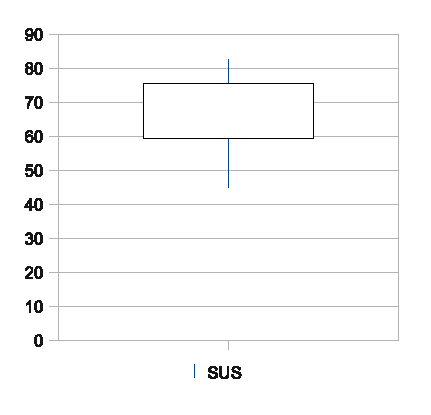
\includegraphics[scale=0.700]{images/aceitacaoSumario.eps}
    }
    \caption{Resultados do formulário SUS.}
    \label{fig:SusResultados}
  \end{center}
\end{figure}

%=====================================================================
\subsubsection{Teste estatístico ou teste de hipótese}
\label{hypothesisTest}
%=====================================================================

Considerando que $H_0: k = 0$,  isto é, a hipótese depende do valor de
$k$,  a  primeira  coisa  a   se  fazer  foi  realizar  o  cálculo  do
coeficiente,    cuja    fórmula    de    cálculo   foi    dada    pela
equação~\ref{eq:Kappa},                 apresentada                 na
seção~\ref{hypothesisFormulation}.   Assim,  seguem  os  cálculos  dos
elementos:

\begin{displaymath}
  p_{o} = 
  \frac{acertos}{acertos + erros} =
  \frac{10}{10 + 4} = 0,7143
\end{displaymath}

\begin{displaymath}
  p_{e} = 
  \displaystyle\sum_{i=1}^{n}(p_{i1} \times p_{i2}) = 
  \left(\frac{5}{14} \times \frac{8}{14}\right) + 
  \left(\frac{5}{14} \times \frac{4}{14}\right) + 
  \left(\frac{4}{14} \times \frac{2}{14}\right) = 0,3469
\end{displaymath}

\begin{displaymath}
  k = \frac{p_{o} - p_{e}}{1 - p_{e}} =
  \frac{0,7143 - 0,3469}{1 - 0,3469} = 0,5625
\end{displaymath}

O valor do coeficiente  é imprescindível para validação dos resultados
do experimento. Contudo, é importante entender o que significa o valor
do  coeficiente obtido,  ou seja,  se o  resultado representa  uma boa
concordância ou não.  Para isso, \citeonline{Landis:Koch:1977} propõem
uma  classificação  desse  valor, atribuindo-lhe  interpretações  mais
descritivas  para  cinco  intervalos,   como  pode  ser  observado  na
tabela~\ref{tab:Agreement}.

\begin{table}[!htb]
 \begin{center}

   \begin{tabular}{cl} \hline

     {\bf Valor de $k$} & {\bf Concordância} \\ \hline
      $<0,00$     & Insignificante \\
      $0,00-0,20$ & Leve \\ 
      $0,21-0,40$ & Razoável \\ 
      $0,41-0,60$ & Moderada \\ 
      $0,61-0,80$ & Substancial \\ 
      $0,81-1,00$ & Quase perfeita \\ \hline

   \end{tabular}
   \caption{Interpretações        para        o        valor        do
     coeficiente~\cite[p.~165]{Landis:Koch:1977}.}
   \label{tab:Agreement}
 \end{center}
\end{table}

A partir do valor de  $k$, procedeu-se aplicação do teste estatístico,
que  foi o  {\em teste  mono-caudal à  direita}, cujos  resultados são
apresentados na  tabela~\ref{tab:Teste}.  Considerando que  o valor de
$k$, obtido, foi  0,5625 e que o valor de P  foi de 0,0020 ($P<0,05$),
com  intervalo de  confiança (95\%)  entre  0,2001 e  0,9249, o  teste
estatístico permitiu que a hipótese nula fosse {\bf rejeitada}.

\begin{table}[!htb]
  \begin{center}

    \begin{tabular}{|m{37mm}|m{20mm}|} \hline
      Coeficiente Kappa & 0,5625 \\ \hline
      $z$                 & 2,8876 \\ \hline
      P                   & 0,0019 \\ \hline
      Intervalo de confiança (95\%)~$\alpha=0,05$ & 
      {\em sup}: 0,9249 {\em inf}:~~~0,2001 \\ \hline
    \end{tabular}
    \caption{Resultado do teste estatístico.}
    \label{tab:Teste}
  \end{center}
\end{table}

%=====================================================================
\section{Considerações sobre o experimento}
\label{inspectionClosures}
%=====================================================================

O  experimento  consistiu  da  realização  da inspeção  de  um  modelo
\aladim, usando  as diretrizes do método  e com o  objetivo de apontar
potenciais problemas de  usabilidade presentes no processo interativo.
O  modelo  utilizado  representa  um  cenário de  uso  de  um  sistema
existente.    Os  resultados  desta   etapa  foram   confrontados  aos
resultados de um teste de  usabilidade executado na interface do mesmo
sistema,  que serviram  de  {\em gabarito}.   Após  isso, uma  análise
estatística  permitiu   verificar  se  os   problemas  de  usabilidade
identificados   durante   as   inspeções   do  modelo   foram   também
identificados nos testes com usuários.

Após  análise  dos  resultados,  obtidos com  as  avaliações,  pôde-se
perceber  que o  método de  inspeção mostrou-se  satisfatório,  pois o
valor  do {\em  Coeficiente  Kappa}~\cite{Cohen:1960}, utilizado  para
medir o  grau de concordância,  foi $k=0,5625$, o que  caracteriza uma
concordância     {\em    moderada},    conforme     a    classificação
de~\citeonline{Landis:Koch:1977},            apresentada            na
tabela~\ref{tab:Agreement}.  No que se  refere ao grau de aceitação, o
resultado  também foi  modesto, pois  a  média do  grau de  aceitação,
calculada a  partir das avaliações  dos participantes, foi  $66,88$, o
que  significou um  grau moderado,  por estar  situado entre  {\em OK}
(50,9)  e  {\em Good}  (71,4),  de  acordo  com as  escalas  propostas
por~\citeonline[p.~118]{Bangor:etal:2009}.

Portanto, com este experimento foi  possível constatar que o método de
inspeção   \aladim\  possibilitou   a  descoberta   de   problemas  de
usabilidade, ainda em fase de design,  o que pode reduzir o impacto de
grandes  mudanças no  código da  aplicação só  nas fases  de  teste de
interface  e aceitação, como  demostrado por~\citeonline{Folmer:2004}.
Contudo, como  toda avaliação  formativa, os avaliadores  apenas atuam
como  potenciais  usuários  e  a  inspeção  resulta,  na  verdade,  em
potenciais problemas de usabilidade,  que seriam constatados durante a
interação.

%%% Local Variables: 
%%% mode: latex
%%% TeX-master: "main"
%%% End: 
	% Inspeção em modelos ALaDIM
%=====================================================================
\chapter{Avaliação (Provas de Conceito)}
\label{Evaluations}
%=====================================================================
Em construção!!!

%%=====================================================================
\section{Estudo de Caso}%5.1
%\label{cdn}
%%=====================================================================
%

Em construção!!!


%%=====================================================================
\subsection{To Publish Music}%5.1.1
%\label{cdn}
%%=====================================================================
%

Refazendo!!!

%Considere o seguinte cenário, uma organização quer prover um serviço para publicação de musica denominado “To Publish Music”. Este serviço monitora durante determinados períodos de tempo a lista de musica de um usuário e publica em ambas as redes sociais do Twitter e Facebook, o titulo da musica que o usuário esta ouvindo no momento pelo Spotify. 
%
%O usuário pode baixar a música que ele está escutando através de um processo de download após a confirmação do pagamento da música ter sido feito ao spotify via PayPal ou cartão de crédito. As funcionalidades de buscar música, escolher música, baixar música, ouvir música, comprar música e publicar música estão disponíveis via “To Publish Music” uma vez que a aplicação esteja implementada de fato. Este estudo de caso tem como desafio garantir a conformidade entre a especificação e o resultado da implementação.

%%=====================================================================
%\subsubsection{$\pi$-ServiceComposition Model}
%%\label{cndDimentions}
%%=====================================================================
%
%Em construção!!!
%
%%O To Publish Music utiliza quatro colaboradores de negócios (Business Colaborator) externos para a construção desta composição de serviços, são eles: Bank, Spotify, Twitter e Facebook;
%%A Figura 4.3 ilustra os serviços do To Publish Music que consistem em um conjunto de funções: busca de música, seleccione a música, comprar música, download de músicas, ouvir música e publicar música. A ação música publish chama dois colaboradores de serviços (Facebook e Twitter), e a ação buy música chama duas funções do colaborador serviço do Banco.
%%
%%\figura{To Publish Music $\pi$-ServiceComposition Model. \cite{Placido}}
%%       {fig:Sign:Peirce}
%%       {BC.png}
%%       {0.500}
%%       {0}
%       
%%%=====================================================================
%%\subsubsection{BPEL Executable Model}
%%%\label{cndDimentions}
%%%=====================================================================
%
%Em construção!!!
%
%
%%Os quatro colaboradores de negócios $\pi$-ServiceComposition Model, serão transformados em quatro parceiros de negócios no BPEL Executable Model: Bank, Spotify, Twitter e Facebook;
%%
%%\figura{Modelo To Publish Music modelado no plugin BPELExecutable.}
%%       {fig:Sign:Peirce}
%%       {BPELModel.png}
%%       {0.500}
%%       {0}
%
%%%%% Local Variables: 
%%%%% mode: latex
%%%%% TeX-master: "main"
%%%%% End: 
%



%%=====================================================================
\subsection{Crime Map}%5.1.2
%\label{cdn}
%%=====================================================================
%

Em construção!!!

%%=====================================================================
\subsection{GesIMED}%5.1.1
%\label{cdn}
%%=====================================================================
%

Em construção!!!

%%=====================================================================
\section{Resultados}%5.1.1
%\label{cdn}
%%=====================================================================
%


Atualmente empresas disponibilizam seu serviços pela internet para facilitar a troca de informações entre empresas e seus clientes . Partindo desta afirmação aplicações são construídas através da composição de serviços distintos de acordo com as necessidades (requisitos) da empresa. Para que estas aplicações garantam algum tipo de qualidade, as   necessidades ou requisitos especificados pela empresa devem ser perfeitamente implementados para que haja uma satisfação subjetiva da empresa que requiriu o sistema. Atingir certo ponto de coerência entre requisitos e implementação não é uma atividade trivial para desenvolvedores. Além disso, os desenvolvedores contam com um grande número de linguagens que orquestram serviços para construir tais aplicações, como por exemplo WS-BPEL 2.0.

Este trabalho tem como objetivo principal complementar a metodologia $\pi$-SOD-M, para que
o mesmo forneça um meio de especificar aplicações baseadas em serviços na linguagem de orquestração de serviços WS-BPEL 2.0. O trabalho libera os desenvolvedores de detalhes específicos da plataforma WS-BPEL promovendo a especificação de aplicações através da modelagem, permitindo que requisitos funcionais sejam modelados através de composição de serviços. Estes requisitos são parte de uma especificação de processos de negócios, ao longo das fases da metodologia, as regras de negócio e assim como as restrições são modeladas utilizando conceitos mais concretos que conduzam a sua implementação em código executável.

Os benefícios de se trabalhar a partir destes resultados propõe um meio de fornecer uma metodologia orientada software que podem ser incluídas em diferentes fases de desenvolvimento, como na especificação das propriedades funcionais, na sua modelagem e implementação. Desta maneira, este trabalho complementa $\pi$-SOD-M proporcionando um ambiente de modelagem de aplicações composta por serviços para a plataforma WS-BPEL 2.0, este mesmo ambiente é capaz de
transformar modelos criados através da modelagem em BPEL e transforma-los em código de
aplicações executáveis.




%=====================================================================
\section{Principais contribuições}
\label{contributions}
%=====================================================================

As principais contribuições desse trabalho são as:

\begin{itemize}

\item[•] A integração das atividades de modelagem de composição de serviços em WS-BPEL 2.0, arquitetura orientada a serviço através de transformações baseadas em modelos

\item[•] A geração de um meta-modelos WS-BPEL 2.0.

\item[•] Especificação de regras de transformação entre $\pi$-ServiceCompositionModel e
WS-BPEL 2.0, procurando expressar, em todas as atividades, as informações contidas na atividade predecessora.

\item[•] Implementação das regras de transformação em ATL permitindo que ocorra um processo automatizado de transformações entre os modelos da atividade supracitada. O processo automatizado permite que sejam mantidas as informações

\item[•] O complemento de um ambiente integrado, $\pi$-SOD-M, que permite a criação de modelos com base em metamodelos bem definidos e regras de transformação entre seus elementos agora para a plataforma WS-BPEL2.0. Tal ambiente facilita o acesso às informações aos modelos gerados pela metodologia e originados durante o processo de desenvolvimento, permitindo que requisitos possam ser adicionados e propagados facilmente para a construção de aplicações em WS-BPEL 2.0. Além disso, oferece
suporte a rastreabilidade entre os modelos.

\item[•] A validação das regras de transformação usando o estudos de caso, o To Publish Music, usado para avaliar se os requisitos estão de acordo com as estratégias de composições geradas orientadas a serviços.

\end{itemize}


%=====================================================================
\section{Trabalhos futuros}
\label{perspectives}
%=====================================================================

À pesquisa desenvolvida nessa dissertação, tem alguns trabalhos futuros que podem ser relacionados, tais com:

\begin{itemize}

\item[•] A extensão do meta-modelo  WS-BPEL 2.0 para que o mesmo dê suporte a politicas de serviços web;

\item[•] Implementar alterações em uma das \textit{engines} de código livre existente para suportar a execução de composições com politicas de serviço.


\item[•] Utilização de métricas para avaliar os resultados das transformações criadas, e a conformidade entre os modelos gerados. As possíveis métricas a serem utilizadas como base, são as fornecidas pelo documento \textit{Model Driving Development} da  \textit{Engineering metrics Baseline}.


\item[•] Especificação e construção de um ambiente de configuração e reconfiguração dinâmica que providencie suporte a transformações orientadas a serviços entre as fases do ciclo de desenvolvimento de software.

\end{itemize}



%%% Local Variables: 
%%% mode: latex
%%% TeX-master: "main"
%%% End: 
		% Considerações finais

%=====================================================================
% Conteúdo pós-textual
%---------------------------------------------------------------------
% Incluindo as referências bibliográficas
%---------------------------------------------------------------------
%\nocite{*}			% listando todo o arquivo .bib 
\bibliography{main}		% arquivo .bbl
%---------------------------------------------------------------------
% Documento estruturado com apêndices, um arquivo para cada apêndice
%---------------------------------------------------------------------
%\appendix
%\include{pos-textual/apendice1}	% Apêndice número 1
%\include{pos-textual/apendice2}	% Apêndice número 2
%=====================================================================
% Fim do documento
%---------------------------------------------------------------------
\label{final}					% referência para a última página
%---------------------------------------------------------------------
\end{document}
%=====================================================================
